\documentclass[a4paper,twoside]{article}
\usepackage{amsmath, amsthm, amssymb}
\usepackage[T1]{fontenc}
\usepackage[bahasa]{babel}
\usepackage{color} %warna
\usepackage{graphicx}
\usepackage{graphics}
\usepackage{float}
\usepackage[cm]{fullpage}
\pagestyle{myheadings}
\usepackage{etoolbox}
\usepackage{setspace} 
\usepackage{lipsum} 
\usepackage{listings} %source code
\usepackage{lscape} %landscape untuk source code
\usepackage{multicol} %multiple column
\usepackage{ifthen} % if then
\setlength{\headsep}{30pt}
\usepackage[inner=2cm,outer=2.5cm,top=2.5cm,bottom=2cm]{geometry} %margin
% \pagestyle{empty}
\usepackage{url}
% \pagestyle{empty}

\makeatletter
\renewcommand{\@maketitle} {\begin{center} {\LARGE \textbf{ \textsc{\@title}} \par} \bigskip {\large \textbf{\textsc{\@author}} }\end{center} }
\renewcommand{\thispagestyle}[1]{}
\markright{\textbf{\textsc{Laporan Perkembangan Pengerjaan Skripsi\textemdash Sem. Genap 2015/2016}}}

\onehalfspacing
 
\begin{document}

\title{\@judultopik}
\author{\nama \textendash \@npm} 

%ISILAH DATA DATA BERIKUT INI:
\newcommand{\nama}{Adriani Sukamto}
\newcommand{\@npm}{2012730045}
\newcommand{\tanggal}{09/05/2016} %Tanggal pembuatan dokumen
\newcommand{\@judultopik}{SPK Pemilihan Nama Baptis Katolik} % Judul/topik anda
\newcommand{\kodetopik}{CEN4004*}
\newcommand{\jumpemb}{1} % Jumlah pembimbing, 1 atau 2
\newcommand{\pembA}{Cecilia Esti Nugraheni}
\newcommand{\pembB}{-}
\newcommand{\semesterPertama}{40 - Genap 15/16} % semester pertama kali topik diambil, angka 1 dimulai dari sem Ganjil 96/97
\newcommand{\lamaSkripsi}{1} % Jumlah semester untuk mengerjakan skripsi s.d. dokumen ini dibuat
\newcommand{\kulPertama}{Skripsi 1} % Kuliah dimana topik ini diambil pertama kali
\newcommand{\tipePR}{B} % tipe progress report :
% A : dokumen pendukung untuk pengambilan ke-2 di Skripsi 1
% B : dokumen untuk reviewer pada presentasi dan review Skripsi 1
% C : dokumen pendukung untuk pengambilan ke-2 di Skripsi 2
\maketitle

\pagenumbering{arabic}

\lstset{
  numbers=left,
  stepnumber=1,    
  firstnumber=1,
  numberfirstline=true
}
\lstset{basicstyle=\tiny, commentstyle=\color{blue}}
\lstset{frame=leftline, tabsize=4, breaklines=true}

\section{Data Skripsi} %TIDAK PERLU MENGUBAH BAGIAN INI !!!
Pembimbing utama/tunggal: {\bf \pembA}\\
Pembimbing pendamping: {\bf \pembB}\\
Kode Topik : {\bf \kodetopik}\\
Topik ini sudah dikerjakan selama : {\bf \lamaSkripsi} semester\\
Pengambilan pertama kali topik ini pada : Semester {\bf \semesterPertama} \\
Pengambilan pertama kali topik ini di kuliah : {\bf \kulPertama} \\
Tipe Laporan : {\bf \tipePR} -
\ifdefstring{\tipePR}{A}{
			Dokumen pendukung untuk {\BF pengambilan ke-2 di Skripsi 1} }
		{
		\ifdefstring{\tipePR}{B} {
				Dokumen untuk reviewer pada presentasi dan {\bf review Skripsi 1}}
			{	Dokumen pendukung untuk {\bf pengambilan ke-2 di Skripsi 2}}
		}

\section{Detail Perkembangan Pengerjaan Skripsi}
Detail bagian pekerjaan skripsi sesuai dengan rencan kerja/laporan perkembangan terkahir :
	\begin{enumerate}
		
		\item Melakukan wawancara ke Romo atau Pastor mengenai syarat apa saja yang diperlukan untuk memilih nama baptis.\\
		{\bf status :} Ada sejak rencana kerja skripsi.\\
		{\bf hasil :} Dalam menganalisis kebutuhan pemilihan nama baptis Katolik, peneliti melakukan wawancara dengan Pastor Paroki St. Laurentius, A. Boogaarts, OSC (Lampiran \ref{fig:bukti}: Bukti Wawancara). Wawancara sudah dilakukan pada tanggal 3 Maret 2016. Wawancara dengan Pastor Paroki bertujuan untuk mengetahui secara mendetail atau terperinci mengenai pembaptisan dalam agama Katolik. Wawancara dilakukan dengan cara menanyakan beberapa butir pertanyaan kepada Pastor A. Bogaartz, OSC sebagai Pastor Paroki di Gereja St. Laurentius. Setelah melakukan wawancara, penulis mendapatkan penjelasan secara umum mengenai Sakramen Baptis, nama Baptis, serta cara pemilihan nama baptis. Berikut adalah beberapa pertanyaan yang diajukan:
		
		\begin{enumerate}
		\item Apa makna baptis untuk agama Katolik?
		\item Kenapa harus ada nama baptis?
		%\item Bagaimana cara pembaptisan dalam agama Katolik?
		%\item Lebih baik baptis pada waktu bayi atau dewasa?
		\item Apakah memilih nama baptis ada kriteria tertentu?
		\end{enumerate}
		
		Berdasarkan hasil wawancara dengan Pastor Paroki, Pastor A. Bogaarts, OSC, berikut adalah penjelasan secara umum mengenai Baptis, nama Baptis, serta cara pemilihannya:
\begin{enumerate}
	\item Makna baptis untuk agama Katolik adalah suatu lambang lahiriah di mana diungkapkan, bahwa menjadi anggota gereja Katolik yang secara resmi adalah diangkat menjadi anak Allah.
	\item Tidak harus ada nama baptis. Tetapi nama baptis merupakan suatu tradisi sebagai ungkapan bahwa di dalam baptisan itu dikuduskan dengan harapan tidak sembarangan memilih nama baptis, tetapi lebih ingin meniru teladan orang kudus yang dia pilih sebagai nama baptis, sehingga menjadi kudus dengan nama baptis yang dia pilih.
		%\item Cara pembaptisan dalam agama Katolik selain disiram dengan air adalah ditenggelamkan/ dibenamkan/ dicelupkan menggunakan air yang mengalir yang telah diberkati (air percikan tidak cukup).
		%\item Ada beberapa kelemahan ketika baptis waktu bayi, yaitu kurangnya mendapatkan pendalaman iman. Tetapi ada keuntungannya juga, yaitu telah mengikut Yesus Kristus dari sewaktu Bayi. Sedangkan jika baptis dewasa, yaitu benar-benar belajar dengan cara mencari komunitas/ dapat membantu dia memilih Yesus Kristus sebagai Juru Selamat serta Kitab Suci dan sebagainya.
		\item Pemilihan nama baptis tidak ada kriteria (bebas memilih), tetapi sebaiknya kita memilih nama baptis yang mempunyai arti sesuai dengan pribadi dari calon baptis. Tanggal lahir, tanggal pembaptisan, serta tanggal pesta santo-santa (peringatan) juga bisa dijadikan acuan dalam memilih nama baptis.
\end{enumerate}
		
		\item Membuat Kuesioner dan menyebarkannya di kalangan gereja maupun orang-orang Katolik.\\
		{\bf status :} Ada sejak rencana kerja skripsi.\\
		{\bf hasil :} Survei sudah dilakukan pada tanggal 7 Februari 2016. Survei dilakukan dengan cara menyebarkan kuisioner ke berbagai kalangan Katolik melalui sebuah link google form. Pada Google Form, terdapat lima pertanyaan. Berikut adalah pertanyaan dari formulir kuesioner pemilihan nama baptis Katolik (Lampiran \ref{fig:formkuesioner}: Formulir Pertanyaan Kuesioner).

\begin{enumerate}
	\item Apakah anda seorang Katolik?
	
	Pertanyaan ini dibuat dengan tujuan agar penulis dapat mengetahui persentase \textit{user} yang mengisi beragama Katolik atau calon Katolik. Yang dimaksud calon Katolik adalah orang yang ingin masuk ke dalam agama Katolik atau mengikuti Kristus sebagai Juru Selamat-Nya. Penulis memberikan sebuah pilihan untuk jawaban pertanyaan ini, yaitu ya dan tidak. Jika \textit{user} mengisi dan jawabannya adalah ya, maka \textit{user} dapat membantu dalam hal analisis kebutuhan pemilihan nama baptis. %Jika \textit{user} mengisi dan jawabannya adalah Tidak, maka \textit{user} dapat menambah pengetahuan \textit{user} mengenai pemilihan nama baptis. 
	\item Jika jawaban anda Ya, apakah anda sudah dibaptis?
	
	Pertanyaan ini dibuat dengan tujuan agar penulis dapat mengetahui persentase \textit{user} yang sudah dibaptis. Penulis memberikan sebuah pilihan untuk jawaban pertanyaan ini, yaitu sudah dan belum. Jika \textit{user} mengisi dan jawabannya adalah sudah, maka \textit{user} dapat membantu dalam hal analisis kebutuhan pemilihan nama baptis. %Jika penulis sudah mengetahui presentasi yang dibaptis, maka dapat membantu dalam hal analisis kebutuhan pemilihan nama baptis.
	\item Jika sudah, kapan anda telah dibaptis?
	
	Pertanyaan ini dibuat dengan tujuan agar penulis dapat mengetahui persentase \textit{user} yang sudah dibaptis ketika bayi dan juga ketika dewasa. Penulis memberikan sebuah pilihan untuk jawaban pertanyaan ini, yaitu ketika masih bayi dan ketika sudah dewasa.
	%\item Apa yang membuat anda dibaptis?
	
	%Pertanyaan ini dibuat dengan tujuan agar penulis dapat mengetahui alasan yang membuat \textit{user} ingin dibaptis. Jawaban pertanyaan ini berupa teks kosong, sehingga \textit{user} dapat mengisi beberapa alasan secara bebas.
	\item Anda memilih nama baptis tersebut berdasarkan apa saja?
	
	Pertanyaan ini dibuat dengan tujuan agar penulis dapat mengetahui faktor yang patut untuk dijadikan sebagai sebuah kriteria pemilihan nama baptis Katolik. Penulis memberikan beberapa pilihan untuk jawaban pertanyaan ini, yaitu tanggal lahir, tanggal pembaptisan Anda, deskripsi santo-santa (cerita kehidupan santo-santa), tanggal pesta santo-santa (peringatan), profesi santo-santa, arti nama dari santo-santa, lambang dari santo-santa, dan jika \textit{user} ingin menjawab selain pilihan tersebut. Jawaban dengan pilihan yang lain juga dapat dijadikan sebuah kriteria, jika jawabannya masuk akal.
\end{enumerate}

\item Menganalisa kebutuhan berdasarkan hasil wawancara\\
		{\bf status :} Ada sejak rencana kerja skripsi.\\
		{\bf hasil :}	Penelitian ini berfokus pada pembahasan pemilihan nama baptis, untuk itu bagian yang akan dianalisa lebih mendalam adalah pada bagian kriteria pemilihan nama Baptis. Berdasarkan hasil wawancara di atas, dapat dianalisa bahwa nama baptis tidak diharuskan, tetapi nama baptis sudah merupakan sebuah tradisi dalam agama Katolik. Kriteria pemilihan nama baptis yang bisa dijadikan sebuah acuan atau pedoman dalam memilih nama Baptis berdasarkan hasil wawancara adalah sebagai berikut:
	

	\begin{itemize}
		\item Bakat calon Baptis (profesi)
		\item Nama calon Baptis
		\item Tanggal lahir calon Baptis
		\item Tanggal pembaptisan calon Baptis
		\item Tanggal Pesta santo-santa (tanggal peringatan)
		\item Arti santo-santa
	\end{itemize}
		

		\item Menganalisa kebutuhan berdasarkan hasil kuesioner.\\
		{\bf status :} Ada sejak rencana kerja skripsi.\\
		{\bf hasil :}	Penelitian ini berfokus pada pembahasan pemilihan nama baptis, untuk itu bagian yang akan dianalisa lebih mendalam adalah pada bagian kriteria pemilihan nama Baptis. Sampel yang diambil adalah seratus orang yang terdiri dari sembilan puluh enam orang beragama Katolik dan empat orang calon Katolik (Lampiran \ref{fig:kues1}: Hasil Kuesioner, Lampiran \ref{fig:kues2}: Hasil Kuesioner, Lampiran \ref{fig:kues3}: Hasil Kuesioner, Lampiran \ref{fig:kues4}: Hasil Kuesioner, Lampiran \ref{fig:kues5}: Hasil Kuesioner, Lampiran \ref{fig:kues6}: Hasil Kuesioner). Setiap responden ada yang memilih kriteria nama baptis sampai empat atau lima kategori. Kriteria pemilihan nama baptis yang bisa dijadikan sebuah acuan atau pedoman dalam memilih nama Baptis berdasarkan hasil kuesioner adalah sebagai berikut (Gambar \ref{fig:Capture}: Kategori Pemilihan Nama Baptis):
		
\begin{itemize}
			\item Tanggal Lahir sebanyak 11 orang
			\item Tangal Pembaptisan sebanyak 6 orang
			\item Deskripsi atau cerita kehidupan Santo-Santa sebanyak 32 orang
			\item Pesta Santo-Santa sebanyak 1 orang
			\item Profesi Santo-Santa sebanyak 6 orang
			\item Arti Nama Santo-Santa sebanyak 45 orang
			\item Lambang dari Santo-Santa sebanyak 5 orang
			\item Lain-lain sebanyak dua puluh 6 orang
		\end{itemize}
		
	\begin{figure}[htbp]
		\centering
			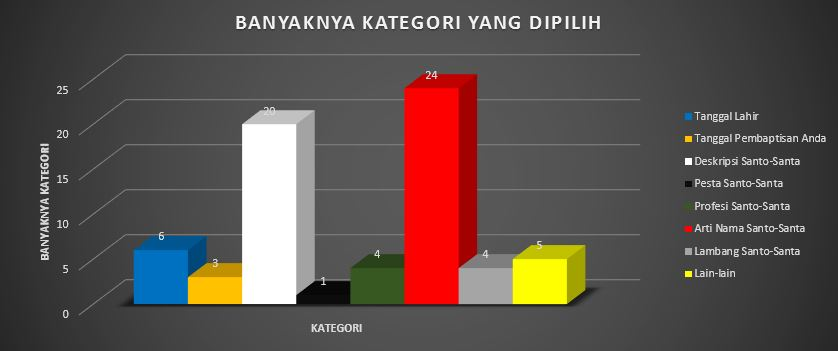
\includegraphics[scale=0.7]{Capture.JPG}
			\caption{Kategori Pemilihan Nama Baptis}
		\label{fig:Capture}
	\end{figure}

	Berdasarkan hasil kuesioner di atas (Gambar \ref{fig:Capture}: Kategori Pemilihan Nama Baptis), dapat di analisa bahwa kriteria yang paling banyak dijadikan acuan (diurutkan berdasarkan responden terbanyak) adalah sebagai berikut:
	
	\begin{itemize}
		\item Kriteria pertama 
		
		Arti Nama Santo-Santa dengan jumlah responden 45 \textit{user}.
		\item Kriteria kedua 
		
		Deskripsi atau cerita kehidupan Santo-Santa dengan jumlah responden 32 \textit{user}.
		\item Kriteria ketiga 
		
		Tanggal lahir calon Baptis dengan jumlah responden 11 \textit{user}.
		\item Kriteria keempat 
			
			Tanggal pembaptisan dan profesi Santo-Santa dengan jumlah responden 6 \textit{user}.
		\item Kriteria kelima
		
		Lambang Santo-Santa dengan jumlah responden 5 \textit{user}.
		\item Kriteria keenam
		
		Pesta Santo-Santa dengan jumlah responden 1 \textit{user}.
	\end{itemize}
	
				
		
		\item Melakukan studi literatur mengenai SPK.\\
		{\bf status :} Baru ditambahkan pada semester ini.\\
		{\bf hasil :} Menurut Raymond McLeod (1998) dalam jurnal Teknik Informatika oleh Verina Valensia dan kawan-kawan bahwa SPK (Sistem Pendukung Keputusan) adalah sebuah sistem penghasil informasi spesifik yang ditujukan untuk memecahkan suatu masalah tertentu yang harus dipecahkan oleh manager pada berbagai tingkatan. Menurut Litle (1970), dalam jurnal Teknik Informatika oleh Verina Valensia dan kawan-kawan bahwa SPK adalah suatu sistem informasi berbasis komputer yang menghasilkan berbagai alternatif keputusan untuk membantu manajemen dalam menangani berbagai permasalahan yang terstruktur dengan menggunakan data dan model. 

Secara umum, SPK adalah sistem yang mampu memberikan kemampuan, baik kemampuan pemecahan masalah maupun kemampuan pengkomunikasian untuk masalah semi-terstruktur. Sedangkan secara khusus, SPK adalah sebuah sistem yang mendukung kerja seorang manager maupun sekelompok manager dalam memecahkan masalah semi-terstruktur. Pemecahan masalahnya adalah dengan cara memberikan informasi ataupun usulan untuk mendapatkan keputusan tertentu. Dapat ditarik kesimpulan, bahwa SPK atau yang biasa disebut DSS (\textit{Decision Support Systems}) adalah bagian dari sistem informasi berbasiskan komputer. SPK digunakan untuk mendukung pengambilan keputusan dalam suatu organisasi atau perusahaan ataupun seseorang. Menurut Moore and Chang, SPK dapat digambarkan sebagai sistem yang berkemampuan mendukung analisis \textit{ad hoc} data, pemodelan keputusan, berorientasi keputusan dan orientasi perencanaan masa depan. Kerangka dasar pengambilan keputusan manajerial dalam tipe keputusan dibagi menjadi:	
	\begin{enumerate}
		\item Keputusan Terstruktur (\textit{structured decision})
		
		Keputusan Terstruktur adalah sebuah keputusan yang berulang-ulang dan rutin, sehingga dapat diprogram. Keputusan terstruktur terjadi dan dilakukan terutama pada manajemen tingkat bawah. Contoh dari keputusan tipe ini adalah keputusan pemesanan barang, keputusan penagihan piutang dan lain sebagainya.
		
		\item Keputusan Tidak Terstruktur (\textit{unstructured decision})
		
		Keputusan Tidak Terstruktur adalah sebuah keputusan yang tidak terjadi berulang-ulang dan tidak selalu terjadi. Keputusan pada tipe ini terjadi dan dilakukan terutama pada manajemen tingkat atas. Informasi tidak mudah didapatkan, tidak mudah tersedia, dan biasanya berasal dari lingkungan luar. Contoh dari keputusan tipe ini adalah keputusan untuk bergabung dengan perusahaan lain.
		\item Keputusan Semi Terstruktur (\textit{semi-structured decision})
		
		Keputusan Semi Terstruktur adalah keputusan yang sebagian dapat diprogram, sebagian dapat berulang-ulang dan rutin, tetapi sebagian tidak terstruktur. Keputusan tipe ini bersifat rumit dan membutuhkan perhitungan serta analisis yang terperinci. Contoh dari keputusan tipe ini adalah keputusan alokasi dana promosi.
	\end{enumerate}
	
	SPK mempunyai beberapa tujuan dalam mendukung suatu keputusan dalam suatu organisasi atau perusahaan ataupun seseorang. Tujuan dari SPK adalah sebagai berikut:
	
	\begin{enumerate}
		\item Membantu menyelesaikan masalah semi-terstuktur
		\item Mendukung manajer dalam mengambil keputusan suatu masalah
		\item Meningkatkan efektifitas bukan efisiensi pengambilan keputusan
	\end{enumerate}

	Dalam sebuah SPK, terdapat \textit{Fuzzy Multiple Attribute Decision Making} (FMADM) yang adalah suatu metode yang digunakan untuk mencari alternatif optimal dari sejumlah alternatif dengan kriteria tertentu. Dalam FMADM, kita dapat menentukan nilai bobot untuk setiap atribut, yang kemudian dilanjutkan dengan proses perankingan yang akan menyeleksi alternatif yang sudah diberikan. Ada beberapa metode yang dapat digunakan untuk menyelesaikan masalah FMADM, antara lain:
	
	\begin{enumerate}
		\item \textit{Simple Additive Weighting Method} (SAW)
		\item \textit{Weighted Product} (WP)
		\item ELECTRE
		\item \textit{Technique for Order Preference by Similarity to Ideal Solution}(TOPSIS)
		\item \textit{Analytic Hierarchy Process}(AHP)
	\end{enumerate}
	
	Ada berbagai macam masalah yang dialami oleh seseorang, perusahaan dan lain-lain dalam kehidupan sehari-hari. Masalah dapat dipecahkan atau dapat diselesaikan dengan baik jika sudah mengerti permasalahan utamanya seperti apa. Jika seseorang ataupun sebuah perusahaan telah mengetahui permasalahan mereka, maka mereka akan membuat sebuah keputusan. Keputusan yang dihasilkan merupakan sebuah keputusan yang terbaik bagi mereka. Adapun tahapannya dalam mengambil sebuah keputusan. SPK mempunyai tahapan proses pengambilan keputusan, diantaranya adalah sebagai berikut:
	\begin{itemize}
		\item Tahap Penelusuran
			
			Tahap ini merupakan proses penelusuran, pendeteksian dari lingkup problematika, serta proses pengenalan masalah. Data yang diperoleh diproses dan diuji dalam rangka mengidentifikasikan masalah.
		\item Tahap Perancangan
		
	Tahap ini merupakan proses menemukan, mengembangkan dan menganalisis tindakan yang mungkin dilakukan. Hal ini meliputi pemahaman terhadap masalah dan menguji solusi yang layak.
		\item Tahap Pemilihan
		
		Pada tahap ini dibuat suatu keputusan yang nyata dan diambil suatu komitmen untuk mengikuti suatu tindakan tertentu.
		\item Tahap Implementasi
		
		Pada tahap ini dibuat suatu solusi yang direkomendasikan dapat bekerja atau implementasi solusi yang diusulkan untuk suatu masalah.
		
	\end{itemize}
	
		Diperlukan tahapan-tahapan diatas karena sebuah masalah atau persoalan mempunyai informasi yang harus dipertimbangkan untuk dipilih menjadi yang terbaik. Oleh karena itu, SPK berbasiskan komputer ini, dapat membantu memecahkan persoalan atau masalah-masalah yang sering dihadapi oleh perusahaan, organisasi ataupun seseorang dengan mengumpulkan data dan mengolahnya menjadi sebuah informasi.
		
		Selain mempunyai tahapan pada pemilihan alternatifnya, SPK juga mempunyai beberapa karakteristik. Karakteristik SPK adalah sebagai berikut:
		
		\begin{enumerate}
			\item Mendukung pengambilan keputusan untuk membahas masalah-masalah terstruktur, semi-terstruktur, dan tidak terstruktur.
			\item Output ditujukan bagi personil organisasi dalam semua tingkatan.
			\item Mendukung masing-masing fase pada proses pengambilan keputusan: penelusuran, perancangan, dan pemilihan.
			\item Adanya antar-muka (\textit{interface}) manusia atau mesin, di mana manusia tetap mengontrol proses pengambilan keputusan.
			\item Menggunakan model matematis dan statistik yang sesuai dengan pembahasan.
			\item Memiliki kemampuan dialog untuk memperoleh informasi sesuai dengan kebutuhan.
			\item Memiliki subsistem-subsistem yang terintegrasi sedemikian serupa, sehingga dapat berfungsi sebagai kesatuan sistem.
			\item Membutuhkan struktur data komprehensif yang dapat melayani kebutuhan informasi seluruh tingkatan manajemen. Data komprehensif adalah data yang memiliki sifat mampu menangkap atau menerima data dengan baik.
			\item Pendekatan \textit{easy to use}. Ciri suatu sistem pendukung keputusan yang efektif adalah kemudahannya untuk digunakan dan memungkinkan keleluasaan pemakai untuk memilih atau mengembangkan pendekatan-pendekatan baru dalam membahas masalah yang dihadapi.
			\item Kemampuan sistem untuk beradaptasi secara cepat, di mana pengambil keputusan dapat menghadapi masalah-masalah baru dan pada saat yang sama dapat menanganinya dengan cara mengadaptasikan sistem terhadap kondisi-kondisi perubahan yang terjadi.
		\end{enumerate}
		
		Dengan demikian, SPK sangatlah berguna dalam kehidupan sehari-hari. Dengan menggunakan SPK, kita dapat memecahkan suatu masalah dengan baik, karena adanya beberapa alternatif solusi yang baik. Alternatif solusi tersebut dapat kita pilih sesuai dengan yang mendekati atau yang sama dengan yang kita inginkan.
		
		\item Melakukan studi literatur mengenai SAW.\\
		{\bf status :} Ada sejak rencana kerja skripsi.\\
		{\bf hasil :} Metode \textit{Simple Additive Weighting} (SAW) sering dikenal dengan metode penjumlahan terbobot. Konsep dasar pada metode SAW adalah mencari penjumlahan terbobot dari rating kinerja pada setiap alternatif pada semua atribut. Metode ini berguna untuk pengambilan keputusan dalam suatu kasus. Perhitungan dengan menggunakan metode SAW ini menghasilkan nilai dari nilai terbesar hingga nilai terkecil. Nilai terbesar yang akan terpilih sebagai alternatif terbaik, selebihnya merupakan nilai terbesar kedua, ketiga, dan seterusnya akan dijadikan sebagai alternatif lain. Metode SAW ini lebih efisien karena waktu yang dibutuhkan dalam perhitungan lebih singkat daripada dengan metode FMADM yang lain, seperti AHP, ELECTRE, dan metode FMADM lainnya. Metode ini membutuhkan proses normalisasi matriks keputusan ke suatu skala yang dapat diperbandingkan dengan semua rating alternatif yang ada. %Proses normalisasi adalah sebuah proses yang mengelompokkan data menjadi satu.

Pada metode SAW, terdapat proses normalisasi. Normalisasi adalah sebuah proses yang menormalisasikan matriks keputusan (X) ke suatu skala, yang dapat diperbandingkan dengan semua rating alternatif yang ada. Dengan kata lain, normalisasi adalah sebuah proses pengelompokkan data menjadi satu kategori dan diperbandingkan. Normalisasi dikelompokkan menjadi 2 atribut, yaitu atribut keuntungan (\textit{benefit}) dan atribut biaya (\textit{cost}). Perbedaan mendasar dari kedua atribut ini adalah dalam pemilihan kriteria. Jika seseorang memilih kriteria yang mengandung sebuah keuntungan, maka akan dilakukan proses normalisasi menggunakan atribut keuntungan, begitu juga sebaliknya. Pada kelompok kedua atribut tersebut dibutuhkan proses normalisasi dengan sebuah formula normalisasi.  Untuk melakukan normalisasi tersebut dibutuhkan sebuah formula sebagai berikut:


\[ r_{ij}  =
  \begin{cases}
    \frac{x_{ij}}{\stackrel{Max}{i} x_{ij}}      & \quad \text{jika } j \text{ adalah atribut keuntungan (\textit{benefit})}\\
		
		
  \frac{\stackrel{Min}{i} x_{ij}} {x_{ij}}     & \quad \text{jika } j \text{ adalah atribut biaya (\textit{cost})}\\
  \end{cases}
\]

%\begin{figure}[htbp]
	%	\centering
		%	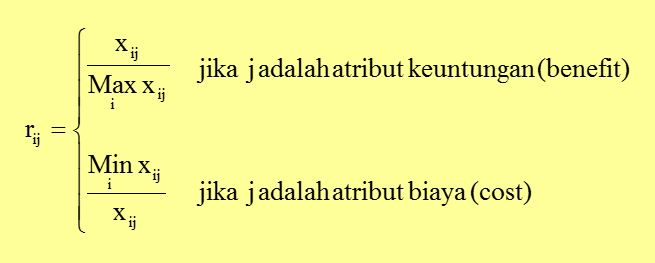
\includegraphics[scale=0.4]{Gambar/saw1.jpg}
		%\caption{Formula Normalisasi}
		%\label{fig:formulanormalisasi}
%	\end{figure}
	
	Keterangan:
	
	\begin{itemize}
		\item $r_{ij}$ = Nilai rating kinerja
		\item $x_{ij}$ = Nilai kinerja dari setiap rating
		\item $Max 	 x_{ij}$ = Nilai terbesar dari tiap kriteria
		\item $Min 	 x_{ij}$ = Nilai terkecil dari tiap kriteria
		\item $i$ = alternatif
		\item $j$ = kriteria
\end{itemize}
	
dengan $r_{ij}$ adalah rating kinerja ternormalisasi dari alternatif ($A_{i}$) pada atribut $C_{j}$; i= 1,2,...,m dan j= 1,2,...,n. Nilai preferensi untuk setiap alternatif diberikan sebagai berikut: 

\[
 V_{i} =\displaystyle\sum_{j=1}^{n} w_{j} r_{ij}
\]

Keterangan:
\begin{itemize}
	\item $V_{i}$ = Nilai akhir dari alternatif
	\item $w_{j}$ = Bobot preferensi atau tingkat kepentingan yang telah ditentukan
	\item $r_{ij}$ = Nilai rating kinerja atau normalisasi matriks
	\item $i$ = alternatif
		\item $j$ = kriteria
\end{itemize}
%\begin{figure}[htbp]
	%	\centering
	%		
\includegraphics[scale=0.4]{Gambar/saw2.jpg}
	%	\caption{Nilai Preferensi}
	%	\label{fig:nilaipreferensi}
%	\end{figure}
	
	Jika telah melalui proses perhitungan, maka ditemukan sebuah hasil Vi. Nilai Vi yang lebih besar mengindikasikan bahwa alternatif Ai lebih terpilih. Langkah-langkah penyelesain dalam menentukan sebuah keputusan dengan menggunakan metode SAW adalah:
	
	\begin{enumerate}
		\item Menentukan alternatif, yaitu $A_{i}$.
		\item Menentukan kriteria-kriteria yang akan dijadikan acuan dalam mengambil keputusan, yaitu $C_{i}$.
		\item Menentukan nilai rating kecocokan setiap alternatif pada setiap kriteria.
		\item Menentukan bobot preferensi atau tingkat kepentingan (W) setiap kriteria. W = [$W_{1}$ $W_{2}$ $W_{3}$ ... $W_{j}$]
		\item Membuat tabel rating kecocokan dari setiap alternatif pada setiap kriteria.
		\item Membuat matriks keputusan X yang dibentuk dari tabel rating kecocokan dari setiap alternatif pada setiap kriteria. Nilai X setiap alternatif ($A_{i}$) pada setiap kriteria ($C_{j}$) yang sudah ditentukan, dimana i=1,2,3,...,m dan j=1,2,3,...,n.
		 \begin{displaymath} X = 
\left (
\begin{array}{rrrr}
X11 & X12 &... &X1j\\		
. & . & . & .\\
. & . & . & .\\
. & . & . & .\\
			Xi1 & Xi2 &... &Xij\end{array}
\right )	
	\end{displaymath}
	\item Melakukan normalisasi matriks keputusan X dengan cara menghitung nilai rating kinerja ternormalisasi ($r_{ij}$) dari alternatif $A_{i}$ pada kriteria $C_{j}$.
	\item Hasil dari nilai rating kinerja ternormalisasi ($r_{ij}$) membentuk matrik ternormalisasi R.\\
	\begin{displaymath} R = 
\left (
\begin{array}{rrrr}
r11 & r12 &... &r1j\\		
. & . & . & .\\
. & . & . & .\\
. & . & . & .\\
			ri1& ri2&... &rij\end{array}\right )	
	\end{displaymath}
	\item Diperoleh hasil dari penjumlahan perkalian elemen baris matrik ternormalisasi R dengan bobot preferensi W yang bersesuaian dengan elemen kolom matrik W. 
	\item Hasil perhitungan nilai $V_{i}$ yang lebih besar mengindikasikan bahwa alternatif $A_{i}$ merupakan alternatif terbaik sebagai solusi.
	\end{enumerate}
	
	Berdasarkan penjelasan yang telah diberikan sebelumnya, dapat disimpulkan bahwa, metode SAW dapat digunakan dalam kehidupan sehari-hari, termasuk dalam menentukan nama baptis pada agama Katolik. Penentuan nama baptis, tidaklah sembarangan. Dalam menentukannya, terdapat beberapa kriteria.

\textbf{Contoh Kasus SAW}
	
	Suatu perusahaan akan memilih seorang karyawan untuk dipromosikan sebagai kepala Cabang \cite{contohsaw}. Perusahaan memberikan empat kriteria yang digunakan untuk melakukan penilaian terhadap calon karyawan. Kriteria ($C_{i}$) diperlukan oleh perusahaan, agar perusahaan dapat menilai calon karyawan yang dijadikan sebagai kandidat alternatif tersebut. Kriteria ditentukan oleh perusahaan berdasarkan beberapa tes dan praktek. Berikut adalah 4 kriteria yang telah ditentukan oleh perusahaan:
\begin{enumerate}
	\item $C_{1}$ = tes pengetahuan (wawasan)
	\item $C_{2}$ = praktek kepemimpinan
	\item $C_{3}$ = tes kepribadian
	\item $C_{4}$ = tes Inovasi
\end{enumerate}
Pada beberapa kriteria yang sudah ditentukan oleh perusahaan tersebut, akan diberikan bobot pada masing-masing kriteria. Berdasarkan metode SAW, bobot diperlukan dalam sebuah kriteria. Bobot ($W_{j}$) pada masing-masing kriteria ditentukan berdasarkan tingkat kepentingan dari setiap kriteria dan harus berjumlah 1 atau 100\%. Bobot tersebut digunakan untuk menghitung nilai akhir dari alternatif. Perusahaan memberikan bobot untuk setiap kriteria sebagai berikut:
\begin{enumerate}
	\item $C_{1}$ = 35\% = 0.35
	\item $C_{2}$ = 25\% = 0.25
	\item $C_{3}$ = 35\% = 0.35
	\item $C_{4}$ = 5\% = 0.05
\end{enumerate}
Selain terdapat kriteria, metode SAW juga membutuhkan sebuah alternatif ($A_{i}$). Alternatif pada perusahaan adalah calon karyawan tersebut. Ada 4 calon karyawan yang menjadi kandidat alternatif untuk dipromosikan sebagai kepala cabang. Alternatif diperlukan oleh perusahaan agar perusahaan dapat mengetahui calon karyawan yang tepat untuk dipromosikan sebagai kepala cabang. Terdapat 2 atribut pada metode SAW, yaitu atribut keuntungan (\textit{benefit}) dan biaya (\textit{cost}). Pada kasus ini, alternatif tersebut termasuk dalam atribut keuntungan, karena hasil \textit{output} yang akan dikeluarkan adalah menguntungkan perusahaan. Berikut adalah 4 alternatif yang sudah terdaftar sebagai calon karyawan di perusahaan tersebut:
\begin{enumerate}
	\item $A_{1}$ = Andre,
	\item $A_{2}$ = Aan,
	\item $A_{3}$ = Andi, dan
	\item $A_{4}$ = Arif.
\end{enumerate}

Pada metode SAW membutuhkan sebuah proses normalisasi. Normalisasi adalah sebuah proses yang menormalisasikan matriks keputusan (X) ke suatu skala, yang dapat diperbandingkan dengan semua rating alternatif yang ada. Dengan kata lain, normalisasi adalah proses pengelompokkan data menjadi satu kategori atribut dan diperbandingkan. Pada kasus ini, data dikelompokkan berdasarkan atribut keuntungan (\textit{benefit}). Pada setiap alternatif yang telah dikelompokkan tersebut, diberikan sebuah angka atau nilai. Angka atau nilai tersebut didapatkan dari hasil tes dan praktek pada kriteria yang ditentukan. Berikut adalah tabel nilai alternatif pada setiap kriteria:
\begin{center}
  \begin{tabular}{|l|r|r|r|r|}  
    \hline
    &
    \multicolumn{4}{|c|}{Kriteria} \\
		\hline
    Alternatif    & $C_{1}$ & $C_{2}$ & $C_{3}$ & $C_{4}$ \\
    \hline
    Andre      & 70&50&80    & 60      \\
       Aan   &    50&60&82&70      \\
    Andi       & 85&55&80&75      \\
    Arif       & 82&75&65&85     \\
    \hline
  \end{tabular}
\end{center}	
Dari data yang sudah didapatkan sebelumnya, maka permasalahan pengambilan keputusan suatu perusahaan dapat diselesaikan. Untuk menyelesaikan permasalahan tersebut dibutuhkan penormalisasian. Berikut adalah rumus normalisasi:

	
	\[ r_{ij}  =
  \begin{cases}
    \frac{x_{ij}}{\stackrel{Max}{i} x_{ij}}      & \quad \text{jika } j \text{ adalah atribut keuntungan (\textit{benefit})}\\
	\end{cases}	  
\]


	Perhitungan dilakukan untuk masing-masing kriteria pada setiap alternatif. Perhitungan dilakukan dengan cara mengambil $x_{ij}$ pada bagian kolom kriteria $C_{i}$ dan nilai maximum (${\stackrel{Max}{i} x_{ij}}$) dari masing-masing kolom pada setiap kriteria. Sebagai contoh, kriteria 1 ($C_{1}$). Pada $C_{1}$, $x_{ij}$ yang akan dihitung pada $r_{11}$ adalah 70, dan kandidat nilai maximumnya (${\stackrel{Max}{i} x_{ij}}$) adalah 70, 50, 85 dan 82. Nilai maximum (${\stackrel{Max}{i} x_{ij}}$) yang didapat adalah 85, sehingga 70 akan dibagi dengan 85. Berikut adalah cara untuk menormalisasikan pada masing-masing kriteria.

	%kolom 1
\begin{enumerate}
	\item Pada $C_{1}$ penyelesaiannya sebagai berikut:
\begin{displaymath}
r_{11} = \frac{70}{max {70;50;85;82}} = \frac{70}{85} = 0.82\\
\end {displaymath}
\begin{displaymath}
r_{21} = \frac{50}{max {70;50;85;82}} = \frac{50}{85} = 0.59\\
\end{displaymath}
\begin{displaymath}
r_{31} = \frac{85}{max {70;50;85;82}} = \frac{85}{85} = 1\\
\end {displaymath}
\begin{displaymath}
r_{41} = \frac{82}{max {70;50;85;82}} = \frac{82}{85} = 0.96\\
\end {displaymath}
%kolom2
\item Pada $C_{2}$ penyelesaiannya sebagai berikut:
\begin{displaymath}
r_{12} = \frac{50}{max {50;60;55;75}} = \frac{50}{75} = 0.67\\
\end{displaymath}
\begin{displaymath}
r_{22} = \frac{60}{max {50;60;55;75}} = \frac{60}{75} = 0.80
\end{displaymath}
\begin{displaymath}
r_{32} = \frac{55}{max {50;60;55;75}} = \frac{55}{75} = 0.73\\
\end{displaymath}
\begin{displaymath}
r_{42} = \frac{75}{max {50;60;55;75}} = \frac{75}{75} = 1
\end{displaymath}
\item Pada $C_{3}$ penyelesaiannya sebagai berikut:
\begin{displaymath}
r_{13} = \frac{80}{max {80;82;80;65}} = \frac{80}{82} = 0.97\\
\end{displaymath}
\begin{displaymath}
r_{23} = \frac{82}{max {80;82;80;65}} = \frac{82}{82} = 1
\end{displaymath}
\begin{displaymath}
r_{33} = \frac{80}{max {80;82;80;65}} = \frac{80}{82} = 0.97\\
\end{displaymath}
\begin{displaymath}
r_{43} = \frac{65}{max {80;82;80;65}} = \frac{65}{82} = 0.79
\end{displaymath}
\item Pada $C_{4}$ penyelesaiannya sebagai berikut:
\begin{displaymath}
r_{14} = \frac{60}{max {60;70;75;85}} = \frac{60}{85} = 0.70\\
\end{displaymath}
\begin{displaymath}
r_{24} = \frac{70}{max {60;70;75;85}} = \frac{70}{85} = 0.82
\end{displaymath}
\begin{displaymath}
r_{34} = \frac{75}{max {60;70;75;85}} = \frac{75}{85} = 0.88\\
\end{displaymath}
\begin{displaymath}
r_{44} = \frac{85}{max {60;70;75;85}} = \frac{85}{85} = 1
\end{displaymath}
\end{enumerate}

Berikut adalah hasil dari nilai rating kinerja yang sudah ternormalisasi:
\begin{displaymath} R = 
\left (
\begin{array}{rrrrrrr}
0.82 & 0.67 & 0.97 & 0.70\\		
0.59 & 0.80 & 1 & 0.82\\
1 & 0 & 0.97 & 0.88 \\
0.96 & 1 & 0.79 & 1 \\
\end{array}\right )	
\end{displaymath}



Proses normalisasi telah selesai dihitung. Dari hasil proses normalisasi didapatkan hasil berupa beberapa data pada masing-masing alternatif terhadap nilai rating kinerja ($r_{ij}$). Pada setiap kriteria terdapat bobot, yaitu W = [$W_{1}$, $W_{2}$, $W_{3}$, $W_{4}$], yang merepresentasikan W = [0.35, 0.25, 0.25, 0.05]. Untuk mendapatkan nilai akhir ($V_{i}$), maka dibutuhkan rumus preferensi, seperti berikut:

\[
 V_{i} =\displaystyle\sum_{j=1}^{n} w_{j} r_{ij}
\]

Perhitungan dilakukan untuk masing-masing alternatif. Sebagai contoh, alternatif 1. Pada alternatif 1, bobot preferensi ($w_{j}$) yang akan dihitung pada nilai akhir ($V_{1}$) adalah 0.35 ($w_{1}$), dan nilai rating kinerja ($r_{ij}$) yang akan dihitung adalah $r_{11}$, $r_{12}$, $r_{13}$, $r_{14}$. Masing-masing $r_{ij}$ pada alternatif 1 akan dikalikan dengan 0.35 dan akan di jumlah. Hasil yang didapat adalah 0.732. Berikut adalah cara untuk mendapatkan nilai akhir pada masing-masing alternatif.

\begin{enumerate}
	\item $V_{1}$ = (0.35)(0.82)+(0.25)(0.67)+(0.25)(0.97)+(0.05)(0.70)= 0.287 + 0.1675 + 0.2425 + 0.035 = 0.732
	\item $V_{2}$ = (0.35)(0.59)+(0.25)(0.80)+(0.25)(1)+(0.05)(0.82)= 0.2065 + 0.2 + 0.25 + 0.041 = 0.6975
	\item $V_{3}$ = (0.35)(1)+(0.25)(0.73)+(0.25)(0.97)+(0.05)(0.88)= 0.35 + 0.1825 + 0.2425 + 0.044 = 0.819
	\item $V_{4}$ = (0.35)(0.96)+(0.25)(1)+(0.25)(0.79)+(0.05)(1)= 0.336 + 0.25 + 0.1975 + 0.05 = 0.8335
\end{enumerate}

Pada nilai akhir ($V_{i}$), nilai yang paling besar dibandingkan nilai yang lain merupakan alternatif terbaik sebagai solusi. Dari hasil perhitungan sebelumnya, didapatkan hasil sebagai berikut:

\begin{center}
    \begin{tabular}{| l | l | }
    \hline
     & Nilai Akhir ($V_{i}$)  \\ \hline
   $V_{1}$ & 0.732 \\ \hline
   $V_{2}$ & 0.6975   \\ \hline
	 $V_{3}$ & 0.819  \\ \hline
   $V_{4}$ & 0.8335   \\ 
    \hline
    \end{tabular}
\end{center}

Jika hasil perhitungan tersebut diurutkan dari yang paling besar hingga paling kecil, maka $V_{4}$ adalah yang paling besar dan $V_{2}$ adalah yang paling kecil. Berikut adalah hasil yang telah diurutkan secara menurun:

\begin{center}
    \begin{tabular}{| l | l | }
    \hline
     & Nilai Akhir ($V_{i}$)  \\ \hline
  $V_{4}$ & 0.8335\\ \hline
	$V_{3}$ & 0.819\\ \hline
	$V_{1}$ & 0.732 \\ \hline
   $V_{2}$ & 0.6975  \\ 
    \hline
    \end{tabular}
\end{center}

Dengan demikian, nilai akhir yang paling besar adalah $V_{4}$, sehingga alternatif $A_{4}$ adalah alternatif yang terpilih sebagai alternatif terbaik. Dengan kata lain, Arif akan terpilih sebagai kepala Cabang. Yang dapat dijadikan alternatif lain setelah $A_{4}$ adalah $A_{3}$, $A_{1}$, dan $A_{2}$.
%dapat disimpulkan bahwa nilai $V_{1}$ adalah 0.732, nilai $V_{2}$ adalah 0.6975, nilai $V_{3}$ adalah 0.819, dan nilai $V_{4}$ adalah 0.8335 \cite{spk2}.  Sehingga nilai akhir yang paling besar adalah $V_{4}$, sehingga alternatif $A_{4}$ adalah alternatif yang terpilih sebagai alternatif terbaik. Dengan kata lain, Arif akan terpilih sebagai kepala Cabang. Yang dapat dijadikan alternatif lain setelah $V_{4}$, adalah $V_{3}$ dengan hasil 0.819, $V_{1}$ dengan hasil 0.732, dan $V_{2}$ dengan hasil 0.6975.

\item Melakukan studi literatur mengenai PHP.\\
		{\bf status :} Ada sejak rencana kerja skripsi.\\
		{\bf hasil :} PHP adalah bahasa pemrograman \textit{script server-side} yang didesain untuk pengembangan web \cite{php2}.  \textit{Script server-side} adalah bahasa pemrograman web yang pengolahan datanya dilakukan oleh komputer server atau penyedia. Jadi, setiap kali sebuah web dikunjungi oleh komputer server akan mengirimkan data-data yang diminta dari database yang kemudian akan ditampilkan di web. Hal ini berbeda dibandingkan dengan bahasa pemrograman \textit{client-side}, seperti JavaScript yang diproses pada web browser (\textit{client}). Selain itu, PHP juga bisa digunakan sebagai bahasa pemrograman umum. Pada awalnya PHP merupakan kependekan dari \textit{Personal Home Page} (Situs Personal). PHP dikembangkan pada tahun 1995 oleh Rasmus Lerdord dan pada waktu itu PHP masih bernama FI (\textit{Form Interpreted}), dan sekarang dikelola oleh \textit{The} PHP \textit{Group}. Situs resmi PHP beralamat di \url{http://www.php.net}.
	
	Pada awalnya PHP merupakan singkatan dari \textit{Personal Home Page}. Sesuai dengan namanya, PHP digunakan untuk membuat website pribadi. Dalam beberapa tahun, PHP berkembang dan menjelma menjadi bahasa pemrograman web yang \textit{powerful} dan tidak hanya digunakan untuk membuat halaman web sederhana, tetapi juga website populer yang digunakan oleh jutaan orang, seperti wikipedia, wordpress, dan lain-lain.
	
	Saat ini PHP adalah singkatan dari \textit{PHP Hypertext Preprocessor}, sebuah kepanjangan rekursif, yakni permainan kata di mana kepanjangannya terdiri dari singkatan itu sendiri. PHP dapat digunakan dengan gratis dan bersifat \textit{open source} dan PHP dirilis dalam lisensi \textit{PHP License}.
	
	Website dinamis yang bisa dibuat menggunakan PHP adalah situs web yang bisa menyesuaikan tampilan konten tergantung situasi. Website dinamis juga bisa menyimpan data ke dalam database, membuat halaman yang berubah-ubah sesuai \textit{input} dari \textit{user}, memproses \textit{form}, dan lain-lain.
	
	Untuk pembuatan web, kode PHP biasanya di sisipkan ke dalam dokumen HTML. Karena fitur inilah, PHP disebut sebagai \textit{\textbf{Scripting Language}} atau bahasa pemrograman \textbf{\textit{script}}. \textit{\textbf{Scripting language}} merupakan penerjemah yang bertugas untuk menerjemahkan dari bahasa yang ada pada web server. \textit{\textbf{Scripting language}} juga dapat dikatakan salah satu komponen pendukung yang paling penting pada web dan terbagi atas dua bagian, yaitu \textit{Client Side Scripting} (CSS) dan \textit{Server Side Scripting} (SSS).

\textbf{Kelebihan PHP}


PHP sudah umum digunakan untuk beberapa web. Dengan demikian, PHP sangat bagus mengenai sistem kerjanya. Sehingga PHP memiliki beberapa kelebihan yang lebih baik, dibandingkan bahasa pemrograman lain, yaitu:
\begin{enumerate}
	\item PHP adalah sebuah \textit{\textbf{Scripting language}} yang tidak melakukan sebuah kompilasi atau kerumitan dalam penggunaannya.
	\item Web Server yang mendukung PHP dapat ditemukan di mana-mana dari mulai apache, IIS, Lighttpd, hingga Xitami dengan konfigurasi yang relatif mudah.
	\item Dalam sisi pengembangan lebih mudah.
	\item Dalam sisi pemahaman, PHP adalah \textit{\textbf{Scripting language}} yang paling mudah karena memiliki referensi yang banyak.
	\item PHP adalah bahasa \textit{open source} yang dapat digunakan di berbagai mesin dan dapat dijalankan secara \textit{runtime} melalui console serta juga dapat menjalankan perintah-perintah sistem.
\end{enumerate}

\textbf{Contoh Kasus PHP}	

	Sebagai contoh kasus penggunaan PHP adalah misalkan kita ingin membuat list dari nomor 1 sampai nomor 10. Tetapi umumnya sebelum menyisipkan PHP pada kode HTML, ada beberapa kode dari HTML murni (belum terdapat kode PHP). Berikut adalah contoh kode untuk membuat list dari nomor 1 sampai dengan nomor 10 menggunakan HTML murni.
	
	\begin{lstlisting}
		<!DOCTYPE html>
		<html>
			<head>
				<title>Contoh list dengan HTML</title>
			</head>
			<body>
				<h2>Daftar Absensi Mahasiswa</h2>
						<ol>
							<li>Nama Mahasiswa ke-1</li>
							<li>Nama Mahasiswa ke-2</li>
							<li>Nama Mahasiswa ke-3</li>
							<li>Nama Mahasiswa ke-4</li>
							<li>Nama Mahasiswa ke-5</li>
							<li>Nama Mahasiswa ke-6</li>
							<li>Nama Mahasiswa ke-7</li>
							<li>Nama Mahasiswa ke-8</li>
							<li>Nama Mahasiswa ke-9</li>
							<li>Nama Mahasiswa ke-10</li>							
						</ol>
			</body>
		</html>
	\end{lstlisting}	
	
	Halaman HTML tersebut dapat dibuat dengan mudah dengan cara melakukan \textit{copy}-\textit{paste} tag\texttt{<li>} sebanyak 10 kali dan mengubah sedikit angka-angka nomor urut di belakangnya. Namun jika yang kita inginkan adalah menambahkan list tersebut menjadi 100 atau 1000 list, cara tersebut menjadi tidak efektif. Jika menggunakan PHP, cara akan menjadi efektif dengan cara membuat perulangan for sebanyak 1000 kali. Berikut adalah contoh kode PHP dengan menggunakan perulangan \texttt{for}.

	\begin{lstlisting}
		<!DOCTYPE html>
		<html>
			<head>
				<title>Contoh list dengan HTML</title>
			</head>
			<body>
				<h2>Daftar Absensi Mahasiswa</h2>
						<ol>
							<?php
									for($i=1;$i<=1000;$i++){
										echo ``<li>Nama Mahasiswa ke-1</li>'';
									}
							?>													
						</ol>
			</body>
		</html>
	\end{lstlisting}	

PHP tidak hanya dapat melakukan pengulangan tersebut, tetapi masih banyak hal 
lain yang bisa dilakukan dengan PHP, seperti menginput data ke database, 
menghasilkan gambar, dan lain sebagainya.

Sama halnya dengan HTML, Java dan kode pemrograman lainnya, PHP juga mempunyai beberapa sintaksis dasar, yaitu:
\begin{itemize}
	\item \texttt{<?php ?>} (Pembatas)
	
	PHP hanya mengeksekusi kode yang ditulis dalam pembatas sebagaimana ditentukan oleh dasar \textit{syntax} PHP. Pembatas yang paling umum adalah ``\texttt{<?php>} '' untuk membuka dan ``\texttt{<?>}'' untuk menutup kode PHP. Tujuan dari pembatas ini adalah untuk memisahkan kode PHP dari kode di luar PHP, seperti HTML, Javascript.	
	\item \texttt{\$ (Variabel)}
	
	Variable diawali dengan simbol dolar \texttt{\$}. Contoh variable dapat ditulis sebagai \texttt{\$nama\_variabel}. Penulisan fungsi, penamaan kelas, nama variable adalah ``peka'' akan huruf besar dan huruf kecil. Kedua kutip ganda \texttt{``  ''} dari string memberikan kemampuan untuk interpolasi nilai variabel ke dalam string PHP. PHP menerjemahkan baris sebagai spasi, dan pernyataan harus diakhiri dengan titik koma. %\semicolon.
	
	\item \texttt{/*   */, //, \# (Komentar)}
	
	PHP memiliki tiga jenis \textit{syntax} sebagai komentar pada kode yaitu:
	
	\begin{itemize}
		\item Tanda blok \texttt{/*   */}, untuk komentar 1 blok
		\item Komentar dua baris \texttt{//}, untuk komentar 2 baris
		\item Tanda pagar \texttt{\#}, untuk komentar satu baris
	\end{itemize}
	Komentar bertujuan untuk meninggalkan catatan pada kode PHP dan tidak akan diterjemahkan ke program.
	\item \texttt{Fungsi}
	
	Seiring dengan perkembangan PHP, fungsi memiliki berbagai konvensi penamaan. \textit{Syntax} fungsi adalah seperti di bawah ini:
	
	\begin{lstlisting}
		function tampilkan($data=``'')
		{ if ($data) return $data;
				else return 'Tidak ada data';
		}
		
		echo tampilkan (``isi halaman'') //menjalankan fungsi
	\end{lstlisting}
	\end{itemize}

\item Melakukan studi literatur mengenai MySQL.\\
		{\bf status :} Ada sejak rencana kerja skripsi.\\
		{\bf hasil :} MySQL adalah sebuah perangkat lunak sistem manajemen basis data SQL (\textit{Structured Query Language}) atau DBMS (\textit{Database Manajement System}) yang \textit{multithread} dan \textit{multi-user}. \textit{Multithread} adalah sebuah proses dengan \textit{thread} yang banyak dan dapat mengerjakan lebih dari satu tugas dalam satu waktu, sedangkan \textit{multi-user} adalah dapat dijalankan oleh banyak user dalam satu waktu tanpa mengalami kendala. \textit{Thread} adalah unit terkecil dalam suatu proses yang bisa dijadwalkan oleh sistem operasi.  

MySQL merupakan turunan salah satu konsep utama dalam database, yaitu SQL. SQL adalah sebuah konsep pengoperasian database, terutama untuk pemilihan atau seleksi dan pemasukan data, yang memungkinkan pengoperasian data dikerjakan dengan mudah secara otomatis.

\textbf{Kelebihan MySQL}

Sebagai database server, MySQL dapat dikatakan lebih unggul dibandingkan database server lainnya dalam \textit{query} data. MySQL memiliki beberapa keistimewaan, antara lain:
		
		\begin{enumerate}
			\item Merupakan salah satu perangkat lunak yang \textit{portable}
			
			Dapat berjalan stabil pada berbagai sistem operasi, seperti Windows, Linux, dan lain sebagainya, sehingga hal ini membuat MySQL menjadi lebih baik dari segi efisiensi dan juga fungsionalitas yang lebih baik. MySQL juga dapat dijalankan untuk mengolah database multi platform. 
			
			\item MySQL merupakan salah satu DBMS yang \textit{open source}
			
			MySQL didistribusikan sebagai perangkat lunak \textit{open source}
			dibawah lisensi GPL, sehingga dapat digunakan secara gratis dan tidak diragukan kualitasnya. 
			
			\item \textit{Multi-user}
			
			Dapat digunakan oleh beberapa pengguna dalam waktu yang bersamaan tanpa mengalami masalah atau konflik, seperti crash dan semacamnya.
			
			\item \textit{Perfomance tuning}
			
			MySQL memiliki kecepatan yang menakjubkan dalam menangani \textit{query} sederhana, dengan kata lain dapat memproses lebih banyak SQL per satuan waktu.
			
			\item Memiliki tipe data yang bervariasi
			
			MySQL memiliki ragam tipe data yang sangat kaya, seperti float, double, char, text, date, dan lain-lain. Dengan beragam tipe data yang didukung oleh MySQL, maka perangkat lunak ini dapat dikategorikan atau digolongkan sebagai salah satu jenis perangkat lunak yang sangat berguna untuk kebutuhan DBMS.
			
			\item Perintah dan fungsi
			
			Memiliki beberapa operator dan fungsi secara penuh yang mendukung perintah \texttt{Select} dan \texttt{Where} dalam perintah (\textit{query}).
			\item Memiliki fitur keamanan yang baik
			
			Memiliki beberapa lapisan keamanan, seperti level subnetmask, nama host, dan izin akses \textit{user} dengan sistem perizinan yang mendetail serta sandi terenkripsi.
			
			\item Skalabilitas dan Pembatasan
			
			MySQL mampu menangani database dalam skala besar. Selain itu batas indeks yang dapat ditampung mencapai 32 indeks pada tiap tabelnya.
			
			\item Konektivitas
			
			MySQL dapat melakukan koneksi dengan klien menggunakan protokol TCP/IP, UNIX, atau NT.
			
			\item Lokalisasi
			
			MySQL dapat mendeteksi pesan kesalahan pada klien dengan menggunakan lebih dari 20 bahasa. 
			
			\item Antar muka (\textit{interface})
			
			Memiliki antar muka (\textit{interface}) terhadap berbagai aplikasi dan bahasa pemrograman dengan menggunakan fungsi API.
			
			\item Klien dan Peralatan
			
			MySQL dilengkapi dengan berbagai peralatan yang dapat digunakan untuk administrasi basis data, dan pada setiap peralatan yang ada disertakan petunjuk \textit{online}.
			
			\item Struktur Tabel yang fleksibel
			
			MySQL memiliki struktur tabel yang lebih fleksibel dalam menangani \texttt{ALTER TABLE}, dibandingkan basis data lainnya.
			
			\item Dapat diintegrasikan dengan berbagai bahasa pemrograman
			
			MySQL dapat membantu pembangunan sebuah sistem dengan mudah dan juga efektif, karena dapat terintegrasikan dengan berbagai macam bahasa pemrograman standar yang dapat digunakan dalam pembangunan suatu sistem.
			
			\item Tidak membutuhkan spesifikasi perangkat keras yang tinggi
			
			Untuk dapat menjalankan program MySQL ini, maka tidak dibutuhkan spesifikasi minimal komputer yang tinggi, sehingga PC ataupun laptop dapat menggunakan perangkat lunak MySQL dengan baik, tanpa menemui kendala dan masalah mengenai spesifikasinya.
			
			\item RAM kecil dapat menggunakannya.
			
			Jika dibandingkan database lain, MySQL dapat dijalankan pada RAM yang relatif kecil. Hanya dengan memory < 1GB pun dapat menggunakannya.
			\end{enumerate}
			
\textbf{Cara Koneksi MySQL ke PHP}

		
		%cara koneksi mysql ke php
Umumnya tampilan web dapat menampilkan data. Data yang ditampilkan tersebut terdapat pada database. Data yang terdapat pada database akan ditampilkan pada tampilan web, jika terdapat kode koneksi seperti berikut.


	\begin{lstlisting}
		<?php
			$servername = ``localhost'';
			$username = ``root'';
			$password = ``'';
			$dbname = ``boostore'';
			
			//create connection
			$conn=new mysqli($servername, $username, $password, $dbname);
			
			//check connection
			if($conn->connect_error){
				die(``Connection failed: '', $conn->connect_error);
			}
		?>
	\end{lstlisting}	

Keterangan:
\begin{itemize}
	\item	\texttt{\$servername} merupakan tempat database berada. Biasanya yang digunakan adalah localhost.
	\item \texttt{\$username} merupakan nama user yang digunakan, biasanya yang digunakan adalah root. Root merupakan sebuah id database yang terdapat di server.
	\item \texttt{\$password} digunakan untuk masuk ke database.
	\item \texttt{\$dbname} merupakan nama database yang terdapat di \texttt{phpMyAdmin}.
\end{itemize}

\item Melakukan studi literatur mengenai bootstrap.\\
		{\bf status :} Ada sejak rencana kerja skripsi.\\
		{\bf hasil :} \textit{Boostrap} adalah \textit{front-end framework} yang bagus, dan luar biasa yang mengedepankan tampilan untuk \textit{mobile device}. Bootstrap berguna untuk mempercepat dan mempermudah pengembangan \textit{website} \cite{bootstrap1}. \textit{Bootstrap} menyediakan HTML, CSS, dan JavaScript yang siap pakai dan mudah untuk dikembangkan.
		
		
		\textit{Bootstrap} merupakan \textit{framework} untuk membangun desain web secara responsif. Tampilan web yang dibuat oleh \textit{bootstrap} akan menyesuaikan ukuran layar dari browser yang kita gunakan baik di \textit{desktop}, \textit{tablet}, ataupun \textit{mobile device}. Dengan \textit{bootstrap} kita juga bisa membangun web dinamis ataupun statis.
		
		Dengan demikian, bootstrap sangat dibutuhkan dan sangat membantu bagi para programmer web. Programmer web tidak perlu membuat atau membangun coding baru lagi untuk setiap \textit{device} yang berbeda, karena tampiannya dapat menyesuaikan ukuran layar.
		
\item Melakukan Analisis database.\\
{\bf status :} Baru ditambahkan pada semester ini.\\
{\bf hasil :} Pada penelitian ini terdapat empat tabel pada sebuah database yang diberi nama ``skripsi2'', yaitu (Gambar \ref{fig:db4}: Desainer Database):
\begin{enumerate}
	\item Tabel nama\_baptis
	\item Tabel kriteria
	\item Tabel kata\_kunci
	\item Tabel kata\_kunci\_nama\_baptis
\end{enumerate}

	\begin{figure}[htbp]
		\centering
			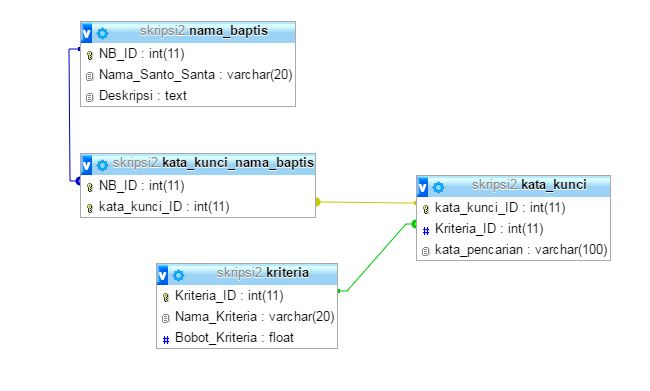
\includegraphics[scale=0.8]{desainerdatabase.JPG}
			\caption{Desain Database}
		\label{fig:db4}
	\end{figure}
	

\textbf{Bagian Tabel nama\_baptis}

Tabel ini digunakan untuk melihat nama baptis, beserta penjelasan detail dari nama baptis tersebut. %makna atau arti, tanggal pesta, nama lain, dan juga lambang dari nama baptis tersebut . 
	Pada tabel nama\_baptis terdapat tiga kolom, yaitu:
	
	
	\begin{itemize}
		\item NB\_ID 
		
		\begin{itemize}
			\item Digunakan untuk memudahkan pengindeksan.
			\item Menggunakan jenis variabel int dengan panjang atau nilai 11.
			\item Merupakan primary key (PK)
			
			PK merupakan nilai unik yang membedakan antara \textit{record} yang 1 dengan yang lain dalam suatu tabel. \textit{Record} adalah struktur data yang menyimpan sekumpulan nilai dari berbagai kolom. Setiap tabel hanya dapat memiliki 1 PK saja. Tetapi jika dalam 1 tabel memiliki lebih dari 1 kolom yang unik, maka dapat digabungkan menjadi sebuah PK yang disebut dengan PK komposit. %PK komposit adalah sebuah PK yang terdiri dari 2 atau lebih kolom.%Jika ingin menyatakan sebuah PK lebih dari 1 kolom%Jika pada tabel terdiri dari lebih dari 1 kolom, maka PK tersebut %PK dapat terdiri dari 1 PK atau banyak PK (disebut PK komposit). %Pada tabel nama\_baptis, PK yang digunakan adalah kunci kandidat (\textit{Candidat Key}). Kunci kandidat merupakan suatu atribut atau satu set minimal atribut yang hanya mengidentifikasikan secara unik untuk suatu kejadian spesifik dari entitas. Secara fungsional, atribut Nama\_Santo\_Santa dan Deskripsi akan bergantung ke atribut NB\_ID.
			%Tabel hanya diperbolehkan memiliki satu PK.
			\item Menggunakan \textit{auto increment}
			
			NB\_ID menggunakan \textit{auto increment}. \textit{Auto increment} merupakan tipe \textit{field} int yang secara otomatis akan bertambah nilainya jika terjadi penambahan \textit{row} pada tabel di mana \textit{field} tersebut berada. Otomatis di sini artinya adalah pada saat memasukkan data baik melalui \textit{statement} INSERT maupun melalui mekanisme data akses lainnya, \textit{field} tersebut tidak perlu dimasukkan nilainya atau cukup diberi nilai NULL, maka MySQL akan menentukan sendiri nilai yang akan diberikan sebagai penambahan baris data tersebut. 
		\end{itemize}
		
		\item Nama\_Santo\_Santa 
				
		\begin{itemize}
			\item Digunakan untuk melihat dan mencatat nama santo-santa atau orang-orang kudus.
			\item Menggunakan jenis variabel varchar dengan panjang atau nilai 20.
		\end{itemize}
		
		\item Deskripsi 
			
		\begin{itemize}
			\item Digunakan untuk melihat penjelasan dari masing-masing santo-santa. Penjelasannya terdiri dari makna atau arti, nama lain santo-santa, lambang, dan tanggal pesta. 
			\item Menggunakan jenis variabel text.
		\end{itemize}
	\end{itemize}


\textbf{Bagian Tabel kriteria}

	Tabel ini digunakan untuk melihat berbagai macam kriteria yang dipilih dan bobot kriteria. Pada tabel kriteria terdapat tiga kolom, yaitu:

\begin{itemize}
	\item Kriteria\_ID 
	
	\begin{itemize}
		\item Digunakan untuk memudahkan pengindeksan.
		\item Menggunakan jenis variabel int dengan panjang atau nilai 11.
		\item Merupakan primary key (PK)
		
			
		\item Menggunakan \textit{auto increment}
		
		%Kriteria\_ID menggunakan \textit{auto increment}. \textit{Auto increment} merupakan tipe \textit{field} int yang secara otomatis akan bertambah nilainya jika terjadi penambahan \textit{row} pada tabel di mana \textit{field} tersebut berada. Otomatis di sini artinya adalah pada saat memasukkan data baik melalui \textit{statement} INSERT maupun melalui mekanisme data akses lainnya, \textit{field} tersebut tidak perlu dimasukkan nilainya atau cukup diberi nilai NULL, maka MySQL akan menentukan sendiri nilai yang akan diberikan sebagai penambahan baris data tersebut.
	\end{itemize}
	
	\item Nama\_Kriteria 
	
	\begin{itemize}
		\item Digunakan untuk mencatat kriteria, seperti arti Santo-Santa, deskripsi, tanggal lahir calon baptis, tanggal pembaptisan, profesi, lambang, serta pesta santo-santa.
		\item Menggunakan jenis variabel varchar dengan panjang atau nilai 20.


	
	\end{itemize}
	\item Bobot\_Kriteria
	
	\begin{itemize}
		\item Digunakan untuk mencatat bobot (W) yang sudah ditentukan untuk masing-masing kriteria.
		\item Menggunakan jenis variabel float, karena mengandung pecahan.
		
	\end{itemize}
\end{itemize}

\textbf{Bagian Tabel Kata\_Kunci}

Tabel ini digunakan untuk melakukan pengelompokkan kata dan dapat yang dicari oleh \textit{user} . Pada tabel kata\_kunci terdapat tiga kolom, yaitu:

	\begin{itemize}
		\item Kata\_kunci\_ID 
		
		\begin{itemize}
		\item Digunakan untuk memudahkan pengindeksan.
		\item Menggunakan jenis variabel int dengan panjang atau nilai 11.
		\item Merupakan primary key (PK)
		
			
		\item Menggunakan \textit{auto increment}
		
		%Kata\_kunci\_ID menggunakan \textit{auto increment}. \textit{Auto increment} merupakan tipe \textit{field} int yang secara otomatis akan bertambah nilainya jika terjadi penambahan \textit{row} pada tabel di mana \textit{field} tersebut berada. Otomatis di sini artinya adalah pada saat memasukkan data baik melalui \textit{statement} INSERT maupun melalui mekanisme data akses lainnya, \textit{field} tersebut tidak perlu dimasukkan nilainya atau cukup diberi nilai NULL, maka MySQL akan menentukan sendiri nilai yang akan diberikan sebagai penambahan baris data tersebut.
		
	\end{itemize}
		
		\item Kriteria\_ID 
		
		\begin{itemize}
			\item Digunakan untuk mengambil data dari tabel kriteria.
			\item Merupakan foreign key (fk) dari tabel kriteria.
			\item Menggunakan jenis variabel int dengan panjang atau nilai 11.
		\end{itemize}
		
		\item Kata\_pencarian 
	
		\begin{itemize}
			\item Digunakan untuk mencari kata yang dimasukkan oleh \textit{user}.
			\item Menggunakan jenis variabel varchar dengan panjang atau nilai 100.
			\item Berisi kata yang sudah dikelompokkan agar memudahkan dalam pencarian. Sebagai contoh adalah kata agung dan besar, kata-kata tersebut sudah dijadikan satu kesatuan atau dikelompokkan, agar jika \textit{user} mencari kata ``besar'' yang tidak ada pada suatu deskripsi pada tabel nama\_baptis, akan tetap keluar sebagai hasil \textit{output}. Hasil \textit{output} yang akan keluar untuk kata ``besar'' adalah deskripsi yang mengandung kata ``agung'', karena kata ``besar'' sudah tersimpan dan sudah dikelompokkan dengan kata ``agung'' pada kata\_pencarian.
			
		\end{itemize}
	\end{itemize}
	
\textbf{Bagian Tabel Kata\_Kunci\_Nama\_Baptis}

Tabel ini digunakan untuk membuat tabel kata\_kunci dengan tabel nama\_baptis menjadi satu, sehingga sistem dapat mengetahui yang \textit{user} \textit{input} atau masukkan pada kata\_pencarian dan mencocokan kata yang dimasukkan \textit{user} tersebut dengan nama\_baptis yang ada pada tabel nama\_baptis. Dengan demikian, hasil alternatif akan keluar sesuai dengan yang diinginkan oleh \textit{user}. Pada tabel Kata\_Kunci\_Nama\_Baptis terdapat dua kolom, yaitu:

	\begin{itemize}
		\item NB\_ID 
		
		\begin{itemize}
		\item Merupakan PK komposit
		\item Merupakan foreign key (fk) dari tabel nama\_baptis
		\item Menggunakan jenis variabel int dengan panjang atau nilai 11.
		\item Digunakan untuk mengambil data dari tabel nama\_baptis
		\end{itemize}
		
		\item Kata\_Kunci\_ID 
		
		\begin{itemize}
		\item Merupakan PK komposit
		\item Merupakan foreign key (fk) dari tabel kata\_kunci
		\item Menggunakan jenis variabel int dengan panjang atau nilai 11.
		\item Digunakan untuk mengambil data dari tabel kata\_kunci
		\end{itemize}
\end{itemize}

	Dari hasil analisis database sebelumnya, dapat disimpulkan bahwa \textit{user} dapat memasukkan \textit{input} berupa kriteria, seperti tanggal lahir calon baptis, tanggal pembaptisan, arti, lambang, profesi dan sebagainya (\textit{input} dapat lebih dari satu). Setelah \textit{user} memasukkan \textit{input} tersebut, maka database akan mencari pada tabel kata\_kunci. Setelah kata yang dicari tersebut sudah ditemukan pada tabel kata\_kunci, kemudian tabel kata\_kunci akan melakukan proses \texttt{JOIN} (penggabungan) dengan tabel kata\_kunci\_nama\_baptis, untuk mendapatkan NB\_ID dan kriteria. NB\_ID didapatkan untuk mencocokkan kata yang dicari oleh \textit{user} dengan nama baptis yang ada pada database (tabel nama\_baptis), sedangkan kriteria didapatkan agar database dapat mengetahui \textit{user} memasukkan \textit{input} berdasarkan kriteria jenis apa. Setelah mendapatkan kriteria dan NB\_ID, kemudian kedua tabel yang sudah di \texttt{JOIN} harus melakukan proses \texttt{JOIN} dengan tabel nama\_baptis, agar mendapatkan nama baptis dan deskripsi yang diinginkan oleh \textit{user}.
	
	\textit{Syntax} \texttt{JOIN} dalam MySQL digunakan untuk menggabungkan beberapa tabel, untuk mendapatkan data. \textit{Syntax} \texttt{JOIN} digunakan pada MySQL karena beberapa tabel dapat digabungkan, sehingga dapat dihasilkan sekumpulan \textit{output} tunggal, dan \textit{syntax} \texttt{JOIN} menghubungkan \textit{record-record} pada setiap tabel.
	
	Hasil pada database merupakan data mentah, dengan kata lain masih belum dapat dikatakan hasil akhir. Data mentah tersebut harus diolah kembali agar mendapatkan hasil yang benar-benar dicari oleh \textit{user}, yaitu dengan menggunakan perhitungan pada metode SAW, dimana membutuhkan bobot pada setiap kriterianya.
	

\item Melakukan studi literatur mengenai Baptis.\\
		{\bf status :} Baru ditambahkan pada semester ini.\\
		{\bf hasil :} Dalam agama Katolik, arti baptis merupakan sebuah sakramen yang berarti upacara suci \cite{sbaptis}. Baptis bukan hanya sekedar upacara belaka. Baptis merupakan awal dari usaha sepanjang hidup untuk berubah, agar dapat bersatu dengan Yesus dan menjadi lebih baik lagi dalam hal apapun. Tujuan dari baptis sendiri akhirnya adalah kita akan berbagi hidup dan kuasa dengan-Nya di dunia dan kelak selama-lamanya di surga. Sakramen baptis bagi umat Katolik menjelaskan bahwa:
\begin{enumerate}
	\item Allah menyelamatkan umat-Nya dengan cara ``Aku di dalam dia dan ia di dalam Aku'' (Yoh 6:56).
	\item Umat-Nya memaklumkan ``Ya, saya mau ``dimasuki'' Tuhan dan ``dimasukkan'' dalam Tuhan, sehingga Citra Allah dipulihkan'' (Yoh 15:5). ``Silahkan menggarap aku'', saya mau menyediakan kerjasama yang baik dengan Tuhan. 
\end{enumerate}

	Dalam sakramen baptis, air dituangkan atas kita. Kita secara perlahan dilebur menjadi satu dalam Kristus, namun kita tidak kehilangan identitas pribadi kita. Kita mempersatukan hidup kita dengan hidup-Nya. Tidak hanya bersatu dengan diri-Nya, tetapi juga menjadi bagian dari-Nya dan Ia juga menjadi bagian dari kita. Pembaptisan hanyalah merupakan awal dari suatu proses hidup untuk bersatu dengan Yesus. Kita tidak hanya bersatu secara fisik, tetapi juga bersatu secara mental dan spiritual. Gereja Katolik mengimani tiga makna air, yaitu:
	
	\begin{enumerate}
		\item Memberi hidup
		\item Membersihkan
		\item Memusnahkan dosa dan kejahatan
	\end{enumerate} 
	
	Yang terpenting dalam pembaptisan adalah membaptis dengan air yang suci atau air bersih, yang bergerak dinamis. Yang dimaksud dinamis adalah mengalir. Air yang mengalir tersebut biasa disebut sebagai ``air hidup''. Mereka juga membutuhkan seorang saksi dalam upacara Sakramen Baptis ini. Sebagai seorang Katolik yang utuh, maka seorang Katolik haruslah dibaptis. Syarat umum dalam Sakramen pembaptisan adalah setidaknya kehidupan calon baptis sudah meniru Tuhan Yesus dan juga ingin bersatu dengan diri-Nya. Seperti dalam Sabda Bahagia (Mat 5:3-12) yang diringkas menjadi Tiga Nasihat Injil adalah:
	
	\begin{itemize}
		\item Berjiwa miskin
		
		Nasihat yang pertama adalah berjiwa miskin. Kemiskinan menyebabkan seseorang merasa menderita, tetapi tidak semua orang yang miskin mendatangkan perasaan itu. Dengan cara menjalani hidup miskin, kita dapat merasa memiliki kekayaan jiwa untuk mendekatkan diri pada Tuhan. Hidupnya bergantung hanya pada Allah bukan pada harta.
		\item Taat
		
		Nasihat yang kedua adalah taat. Kita sebagai manusia mempunyai ``Tuan'' yaitu Allah. kita harus selalu menuruti perintah-Nya dan menjauhi larangan-Nya.
		\item Hidup suci 
		
		Nasihat yang ketiga adalah hidup suci. Hidup suci adalah benar-benar bersih dari dunia gemerlap malam hari (dugem), tidak mengejar kenikmatan diri, serta seutuhnya hidup untuk Tuhan dan sesama.
	\end{itemize}
	
	Seseorang tidak harus dibaptis ketika orang tersebut masih bayi. Ada juga yang dibaptis ketika sudah dewasa. Pembaptisan yang dilakukan pada saat dewasa harus melalui beberapa persyaratan. Selain orang dewasa dan bayi yang harus dibaptis adalah:
	
	\begin{itemize}
		%\item Bayi
		
		%Pada bayi harus dibaptis sesegera mungkin sekitar 2-3 bulan setelah kelahirannya. Syarat mengikuti sakramen baptis untuk bayi adalah orang tuanya harus beragama Katolik dan menanam benih, agar tumbuh jadi pohon besar dan berbuah lebat, serta memiliki tanah yang subur.
		%\item Orang dewasa
	
		%Tidak hanya pada bayi, orang dewasa juga terdapat berbagai persyaratan untuk mengikuti Sakramen Pembaptisan. Syarat mengikuti Sakramen Baptis pada orang dewasa atau orang yang baru masuk katolik adalah:
		
		%\begin{itemize}
			%\item Mengikuti pelajaran agama minimal 12 bulan
			%\item Pengetahuan agama Katolik yang cukup
			%\item Beriman
			%\item Hidupnya meniru Tuhan Yesus
			%\item Kehidupan gereja dan sosialisasi diri sudah baik
		%\end{itemize}
		\item Orang beragama Katolik yang bersekolah di sekolah Katolik
		
		Bersekolah di sekolah Katolik dan orang tersebut beragama Katolik, tetapi belum dibaptis dan ingin dibaptis harus memenuhi beberapa syarat. Syarat untuk mengikuti sakramen baptisnya adalah cukup dengan mengikuti pelajaran agama minimal tujuh bulan.
		
		\item Calon pengantin
		
		Persyaratan pada calon pengantin berbeda dengan orang dewasa. Syarat untuk mengikuti Sakramen Baptis untuk calon pengantin adalah cukup dengan mengikuti pelajaran tidak kurang dari 7 bulan.
		\item Orang yang sudah tua (60 tahun ke atas)
		
		Adapun orang yang sudah tua atau manula yang belum menjadi Katolik dan ingin menjadi Katolik. Syarat mengikuti sakramen baptis untuk orang yang sudah tua atau manula adalah sebagai berikut:
		
		\begin{itemize}
			\item Jika orang tersebut sudah pikun, dapat dibaptis dengan persiapan yang sangat pendek.
			\item Jika orang tersebut belum pikun harus menjalani beberapa persiapan secukupnya, seperti hafal doa-doa, pengetahuan agama yang cukup dan mengikuti kegiatan.
		\end{itemize}
		
		\item Orang gila
		
		Adapun sakramen baptis untuk orang gila.Jika orang gila tersebut, pada waktu tidak gilanya pernah menyatakan ingin mengikut Tuhan atau pernah ke gereja, maka akan dibaptis. Jika orang tersebut tidak pernah menyatakannya, maka tidak akan dibaptis.
		\item Dalam bahaya maut
		
		Dalam bahaya maut, siapapun orangnya dapat segera dibaptis dengan syarat hati orang tersebut suci dan penuh pertobatan, serta orang tersebut ingin beragama Katolik.
		
	\end{itemize} 
	Menurut Pastor A. Bogaarts, OSC sebagai Pastor Paroki di Gereja St. Laurentius, arti atau makna baptis sendiri untuk agama Katolik adalah suatu lambang lahiriah di mana diungkapkan, bahwa untuk menjadi anggota gereja Katolik yang secara resmi adalah diangkat menjadi anak Allah.
	
\textbf{Nama Baptis}

	Nama baptis mengingatkan orang yang dibaptis, bahwa ia tergabung dengan Kristus sebagai bagian dari diri-Nya dan ia didorong untuk hidup sesuai dengan panggilannya sebagai anak angkat Allah. Ia didorong sebagaimana yang ditunjukkan oleh teladan orang kudus, yang namanya diambil oleh ia melalui pembaptisan itu. Orang Katolik tidak diharuskan mempunyai nama baptis, tetapi boleh juga mempunyai nama baptis di bagian depan namanya.
	
	Pemakaian nama orang kudus atau santo-santa sebagai nama baptis sangatlah bermakna, baik, dan dianjurkan oleh Gereja. Gereja menganjurkan adanya nama baptis pada bagian depan nama calon baptis, dengan berbagai alasan tertentu, yaitu:
	
	\begin{itemize}
		\item Pemberian nama santo-santa pada saat pembaptisan adalah dengan maksud bahwa manusia ``lahir'' kembali sebagai manusia baru.
		\item Pemberian nama santo-santa mengingatkan akan adanya persekutuan orang kudus.
		\item Nama santo-santa yang kita ambil sebagai nama baptis dapat dijadikan sebagai santo-santa pelindung, dapat menjadi teladan, sehingga dapat meniru contoh kehidupan santo-santa tersebut dan kita dapat mengamalkan cinta kasih agar kita semakin mendekati Kristus.
	\end{itemize}
	
	
	Dalam memilih sebuah nama baptis yang cocok tidaklah sembarangan. Nama baptis benar-benar dipilih untuk menjadi teladan kita dan semakin dekat dengan Kristus. Dalam memilih nama baptis tidaklah hanya memilih berdasarkan namanya yang sesuai, bagus dan lain sebagainya. Melainkan nama baptis dipilih berdasarkan kriteria arti, lambang, tanggal pesta, ataupun cerita kehidupannya, agar kita sebagai calon baptis dapat mengerti, meneladani, dan dapat mengikuti atau meniru cerita kehidupannya (Lampiran \ref{fig:namabaptis1}: Nama Baptis, \ref{fig:namabaptis2}: Nama Baptis).
	
	Pada umumnya nama baptis mempunyai cerita kehidupan, lambang, arti, dan tanggal pesta santo-santa tersebut. Ada yang lengkap, ada juga yang tidak lengkap. Pada Lampiran \ref{fig:namabaptis1}: Nama Baptis, terdapat nama ``Agata''. Pada nama tersebut terdapat cerita kehidupan dari Agata, arti (A), lambang (L), dan tanggal pesta santo-santa (P) tersebut. Sedangkan pada Lampiran \ref{fig:namabaptis2}: Nama Baptis, terdapat nama ``Agatangelus'', yang pada nama tersebut hanya mengandung cerita kehidupan, arti (A), dan tanggal pesta santo-santa (P).
	
	Arti dan cerita kehidupan pada nama santo-santa sangat penting bagi calon baptis. Calon baptis yang memilihnya dapat mengikuti teladan santo-santa tersebut. Lambang yang dimiliki santo-santa juga dapat menjadi sebuah simbol. Tanggal pesta santo-santa pada nama santo-santa dapat dijadikan sebagai acuan jika orang tersebut ingin memilih nama baptis berdasarkan tanggal lahir ataupun tanggal pembaptisan mereka.
	
	Kriteria yang terdapat pada nama baptis tersebut, hanyalah untuk mempermudah kita dalam memilih nama baptis yang kita pilih. Nama baptis yang memiliki kriteria lengkap akan lebih mudah dalam mempertimbangkan nama tersebut tepat atau tidak untuk kita. Selain dapat mempermudah dalam memilih nama baptis, kita juga dapat mengerti dan mengikuti teladan dari nama santo-santa yang dipilih oleh calon baptis tersebut.
	
\textbf{Calon Baptis}
	
	Untuk menjadi bagian dalam agama Katolik, seseorang harus melalui tahap baptis yang disebut Sakramen Baptis atau Sakramen Pembaptisan. Pembaptisan membebaskan calon baptis dari dosa asal, serta semua dosa pribadi dan dari hukuman akibat dosa-dosa tersebut. Selain membebaskan dari dosa, pembaptisan membuat orang yang dibaptis itu mengambil bagian dalam kehidupan Tritunggal Allah melalui rahmat yang menguduskan. Rahmat yang menguduskan adalah sebuah rahmat pembenaran yang mempersatukan pribadi yang bersangkutan dengan Kristus dan Gereja. Pada proses pembaptisan membutuhkan seseorang yang siap dibaptis dan siap mengikuti Kristus, yaitu calon baptis.
	
	
	Calon baptis adalah orang yang ingin menjadi Katolik, mengikut Kristus, mengikuti teladan-Nya, menjadi bagian dari-Nya, dan ingin bersatu dengan Kristus. Selain diterima sebagai anggota baru pada agama Katolik, para calon baptis juga diajak masuk ke kehidupan yang baru, di mana Kristus menjadi panutan utamanya. 
		
	
	Pada agama Katolik terdapat tiga tahap inisiasi Katolik. Tahap inisiasi Katolik adalah tahap di mana para calon baptis dari yang masih belum menjadi Katolik (calon) sampai menjadi anggota baru di Katolik atau dapat diartikan sebagai penerimaan seseorang masuk ke dalam atau menjadi anggota kelompok tertentu. Tahap inisiasinya adalah \cite{cbaptis}:
	
	\begin{itemize}
		\item Masa pra-katekumenat/simpatisan menjadi katekumen
		
			Pada masa ini, calon baptis mengalami masa pemurnian. Masa pemurnian yang dimaksud adalah calon merasa murni dan dituntut dalam pertobatan dan iman.
		\item Masa katekumen menjadi calon baptis
		
		Pada masa ini, calon baptis mengalami masa pengembangan. Pengembangan tersebut melalui ajaran agama, seperti pembinaan iman di Gereja. Pembinaan iman dimaksudkan agar calon baptis dapat siap secara iman menjadi Katolik dan mengikut Kristus. Selain dibina dan mendapatkan pengajaran, calon baptis juga harus melakukan kewajiban berupa tugas. Tugas yang harus dilakukan oleh calon baptis adalah mencatat ringkasan khotbah pada saat pastor sedang melakukan khotbah dan juga mengumpulkan tanda tangan pastor yang khotbah pada waktu itu.
		\item Masa calon baptis menjadi baptisan baru
		
		Pada masa ini, calon baptis sudah benar-benar siap secara iman untuk mengikuti Kristus dan teladan-Nya. Calon baptis akan menjadi anggota gereja Katolik yang baru.
	\end{itemize}

%\textbf{Cara Pembaptisan}

	%Pada agama Katolik, Sakramen Baptis mempunyai cara tersendiri. Cara pembaptisan pada bayi (Gambar \ref{fig:baptis}: Baptis Bayi) dan orang dewasa (Gambar \ref{fig:baptis1}: Baptis Dewasa) pada dasarnya sama, yaitu pastor ataupun diakon menuangkan air suci pada bagian dahi calon baptis atau menenggelamkan calon baptis dan mengucapkan ``Aku membaptis kamu dalam nama Bapa, Putra dan Roh Kudus'' (Matius 28:19), dengan menggunakan air yang mengalir yang telah diberkati, karena air percikan tidak cukup. Air percikan tidak cukup karena tidak dapat membasuh semua dahi kita, atau tidak membasuh semua tubuh kita.
	
	%Dalam wawancara yang telah dilakukan dengan Pastor A. Bogaarts, OSC, menurut beliau, ada beberapa kelemahan dan keuntungan ketika baptis pada waktu bayi. Kelemahannya adalah kurangnya mendapatkan pendalaman iman. Keuntungannya adalah telah mengikut Kristus dari sewaktu Bayi. Sedangkan jika baptis dewasa, yaitu benar-benar belajar. Yang dimaksud belajar adalah dengan cara mencari komunitas Katolik atau dapat membantu dia memilih Kristus sebagai Juru Selamat dan dapat lebih mendalami iman. Untuk orang dewasa yang ingin dibaptis, harus mengikuti pelajaran agama. Pelajaran agama tersebut juga memberikan tugas, seperti menulis khotbah Pastor, serta mengumpulkan tanda tangan Pastor yang khotbah pada waktu itu.
	
%		\begin{figure}[htbp]
%		\centering
%			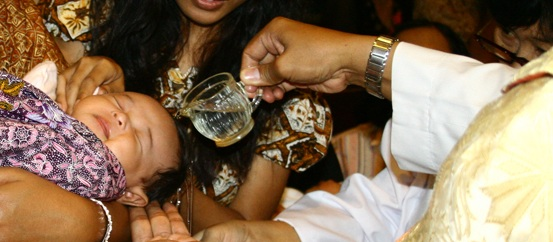
\includegraphics[scale=0.4]{baptis.jpg}
%		\caption{Baptis Bayi}
%		\label{fig:baptis}
%	\end{figure}
	
%	\begin{figure}[ht]
%		\centering
%			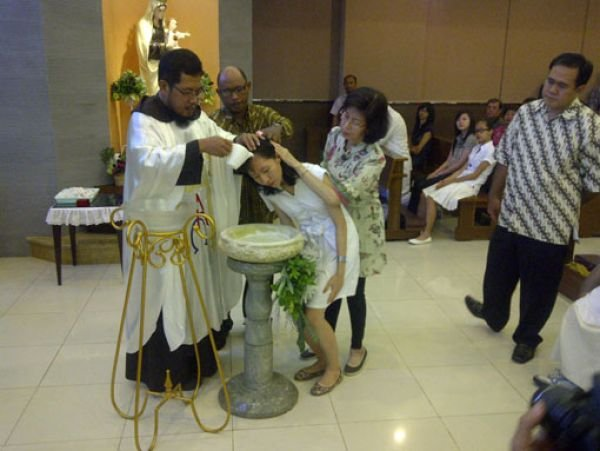
\includegraphics[scale=0.4]{baptis1.jpg}
%		\caption{Baptis Dewasa}
%	\label{fig:baptis1}
%	\end{figure}
		
		
\textbf{Cara Menentukan Nama Baptis}

Dalam menentukan nama baptis tidaklah mudah. Dibutuhkan pengetahuan akan nama-nama baptis Katolik. Menurut Pastor A. Bogaarts, OSC, dalam memilih atau menentukan nama Baptis tidak ada kriteria tertentu atau dapat dikatakan ``bebas memilih'', tetapi sebaiknya kita memilih orang kudus yang sekiranya dekat dengan bakat kita atau nama karena mirip atau memilih karena artinya. Selain itu tanggal lahir, tanggal pembaptisan, serta pesta nama baptis juga bisa dijadikan acuan dalam memilih nama baptis.


\item Melakukan analisis nama baptis menggunakan metode SAW.\\
		{\bf status :} Baru ditambahkan pada semester ini.\\
		{\bf hasil :} Berdasarkan hasil analisis pada subbab analisis wawancara dan subbab analisis kuesioner, didapatkan beberapa kriteria dalam memilih nama baptis pada agama Katolik. Terdapat 7 kriteria $C_{i}$ yang digunakan untuk menentukan nama baptis yang tepat untuk calon baptis. Kriteria diperlukan oleh calon baptis, agar calon baptis dapat menentukan nama baptis yang dijadikan sebagai nama alternatif tersebut. Berikut 7 kriteria $C_{i}$ yang telah ditentukan berdasarkan hasil analisa wawancara dan kuesioner:
\begin{enumerate}
	\item $C_{1}$ = Arti nama santo-santa
	\item $C_{2}$ = Deskripsi atau cerita kehidupan santo-santa
	\item $C_{3}$ = Tanggal lahir calon baptis
	\item $C_{4}$ = Tanggal pembaptisan
	\item $C_{5}$ = Profesi santo-santa
	\item $C_{6}$ = Lambang santo-santa
	\item $C_{7}$ = Tanggal pesta santo-santa
\end{enumerate}
	
		Pada beberapa kriteria yang sudah ditentukan akan diberikan bobot pada masing-masing kriteria. Bobot ($W_{j}$) untuk setiap kriteria adalah sebagai berikut:
		
\begin{enumerate}
	\item $C_{1}$ = 40\% = 0.4
	\item $C_{2}$ = 20\% = 0.2
	\item $C_{3}$ = 10\% = 0.1
	\item $C_{4}$ = 15\% = 0.15
	\item $C_{5}$ = 5\% = 0.05
	\item $C_{6}$ = 5\% = 0.05
	\item $C_{7}$ = 5\% = 0.05
\end{enumerate}

Selain terdapat kriteria, metode SAW juga membutuhkan sebuah alternatif $A_{i}$. Alternatif pada pemilihan nama baptis Katolik adalah nama santo-santa. Ada 10 nama santo-santa yang menjadi nama alternatif untuk dijadikan nama baptis yang tepat oleh calon baptis. Pada pemilihan nama baptis, alternatif tersebut termasuk dalam atribut keuntungan (\textit{benefit}), karena hasil \textit{output} yang akan dikeluarkan adalah menguntungkan calon baptis tersebut.

\begin{enumerate}
	\item $A_{1}$ = Abraham
	\item $A_{2}$ = Adam
	\item $A_{3}$ = Adolf
	\item $A_{4}$ = Agata
	\item $A_{5}$ = Agnes
	\item $A_{6}$ = Agustinus
	\item $A_{7}$ = Brigitta
	\item $A_{8}$ = Daud
	\item $A_{9}$ = Natalia
	\item $A_{10}$ = Yoakim
\end{enumerate}

Pada metode SAW membutuhkan proses normalisasi. Proses normalisasi adalah proses pengelompokkan data berdasarkan atribut. Pada pemilihan nama baptis, data dikelompokkan berdasarkan atribut keuntungan (\textit{benefit}). Pada setiap alternatif yang telah dikelompokkan tersebut, diberikan sebuah angka atau nilai. Angka atau nilai tersebut didapatkan dari hasil \textit{input user} pada kriteria yang ditentukan. Rentang nilai pada masing-masing alteratif pada setiap kata yang dicari adalah 0 sampai 100. Berikut adalah tabel nilai alternatif pada setiap kriteria:
\begin{center}
\begin{tabular}{|l|r|r|r|r|r|r|r|}  
    \hline
    &
    \multicolumn{7}{|c|}{Kriteria} \\
		\hline
    Alternatif    & $C_{1}$ & $C_{2}$ & $C_{3}$ & $C_{4}$ & $C_{5}$ & $C_{6}$ & $C_{7}$ \\
    \hline
    Abraham     & 5&5&5&5&5&5&5     \\ \hline
    Adam	      & 5&5&90&90&5&5&90    \\ \hline
    Adolf       & 5&5&5&5&45&5&5      \\ \hline
    Agata       & 15&30&15&15&15&90&15  \\ \hline
		Agnes    		& 90&30&20&20&20&20&20     \\ \hline
    Agustinus	  & 20&30&20&20&45&20&20    \\ \hline
    Brigitta    & 5&5&5&5&5&5&5      \\ \hline
    Daud       	& 10&10&45&45&10&10&45  \\ \hline
		Natalia     & 25&25&25&25&25&25&25      \\ \hline
    Yoakim      & 5&5&5&5&5&5&5  \\ \hline
    
  \end{tabular}
\end{center}
Dari data yang sudah didapatkan sebelumnya, maka permasalahan pengambilan keputusan calon baptis dapat diselesaikan. Untuk menyelesaikan permasalahan tersebut dibutuhkan penormalisasian. Berikut adalah rumus normalisasi:
	\[ r_{ij}  =
  \begin{cases}
    \frac{x_{ij}}{\stackrel{Max}{i} x_{ij}}      & \quad \text{jika } j \text{ adalah atribut keuntungan (\textit{benefit})}\\
	\end{cases}	  
\]

Perhitungan dilakukan untuk masing-masing kriteria pada setiap alternatif. Perhitungan dilakukan dengan cara mengambil $x_{ij}$ pada bagian kolom kriteria $C_{i}$ dan nilai maximum (${\stackrel{Max}{i} x_{ij}}$) dari masing-masing kolom pada setiap kriteria. Berikut adalah cara untuk menormalisasikan pada masing-masing kriteria.

\begin{enumerate}
%kolom 1
	\item Pada $C_{1}$ penyelesaiannya sebagai berikut:
\begin{displaymath}
r_{11} = \frac{5}{max {5;5;5;15;90;20;5;10;25;5}} = \frac{5}{90} = 0.05\\
\end {displaymath}
\begin{displaymath}
r_{21} = \frac{5}{max {5;5;5;15;90;20;5;10;25;5}} = \frac{5}{90} = 0.05\\
\end{displaymath}
\begin{displaymath}
r_{31} = \frac{5}{max {5;5;5;15;90;20;5;10;25;5}} = \frac{5}{90} = 0.05\\
\end {displaymath}
\begin{displaymath}
r_{41} = \frac{15}{max {5;5;5;15;90;20;5;10;25;5}} = \frac{15}{90} = 0.16\\
\end {displaymath}
\begin{displaymath}
r_{51} = \frac{90}{max {5;5;5;15;90;20;5;10;25;5}} = \frac{90}{90} = 1\\
\end {displaymath}
\begin{displaymath}
r_{61} = \frac{20}{max {5;5;5;15;90;20;5;10;25;5}} = \frac{20}{90} = 0.22\\
\end {displaymath}
\begin{displaymath}
r_{71} = \frac{5}{max {5;5;5;15;90;20;5;10;25;5}} = \frac{5}{90} = 0.05\\
\end {displaymath}
\begin{displaymath}
r_{81} = \frac{10}{max {5;5;5;15;90;20;5;10;25;5}} = \frac{10}{90} = 0.11\\
\end {displaymath}
\begin{displaymath}
r_{91} = \frac{25}{max {5;5;5;15;90;20;5;10;25;5}} = \frac{25}{90} = 0.27\\
\end {displaymath}
\begin{displaymath}
r_{101} = \frac{5}{max {5;5;5;15;90;20;5;10;25;5}} = \frac{5}{90} = 0.05\\
\end {displaymath}

%kolom 2
\item Pada $C_{2}$ penyelesaiannya sebagai berikut:
\begin{displaymath}
r_{12} = \frac{5}{max {5;5;5;30;30;30;5;10;25;5}} = \frac{5}{30} = 0.16\\
\end {displaymath}
\begin{displaymath}
r_{22} = \frac{5}{max {5;5;5;30;30;30;5;10;25;5}} = \frac{5}{30} = 0.16\\
\end{displaymath}
\begin{displaymath}
r_{32} = \frac{5}{max {5;5;5;30;30;30;5;10;25;5}} = \frac{5}{30} = 0.16\\
\end {displaymath}
\begin{displaymath}
r_{42} = \frac{30}{max {5;5;5;30;30;30;5;10;25;5}} = \frac{30}{30} = 1\\
\end {displaymath}
\begin{displaymath}
r_{52} = \frac{30}{max {5;5;5;30;30;30;5;10;25;5}} = \frac{30}{30} = 1\\
\end {displaymath}
\begin{displaymath}
r_{62} = \frac{30}{max {5;5;5;30;30;30;5;10;25;5}} = \frac{30}{30} = 1\\
\end {displaymath}
\begin{displaymath}
r_{72} = \frac{5}{max {5;5;5;30;30;30;5;10;25;5}} = \frac{5}{30} = 0.16\\
\end {displaymath}
\begin{displaymath}
r_{82} = \frac{10}{max {5;5;5;30;30;30;5;10;25;5}} = \frac{10}{30} = 0.33\\
\end {displaymath}
\begin{displaymath}
r_{92} = \frac{25}{max {5;5;5;30;30;30;5;10;25;5}} = \frac{25}{30} = 0.83\\
\end {displaymath}
\begin{displaymath}
r_{102} = \frac{5}{max {5;5;5;30;30;30;5;10;25;5}} = \frac{5}{30} = 0.16\\
\end {displaymath}

%kolom 3
\item Pada $C_{3}$ penyelesaiannya sebagai berikut:
\begin{displaymath}
r_{13} = \frac{5}{max {5;90;5;15;20;20;5;45;25;5}} = \frac{5}{90} = 0.05\\
\end {displaymath}
\begin{displaymath}
r_{23} = \frac{90}{max {5;90;5;15;20;20;5;45;25;5}} = \frac{90}{90} = 1\\
\end{displaymath}
\begin{displaymath}
r_{33} = \frac{5}{max {5;90;5;15;20;20;5;45;25;5}} = \frac{5}{90} = 0.05\\
\end {displaymath}
\begin{displaymath}
r_{43} = \frac{15}{max {5;90;5;15;20;20;5;45;25;5}} = \frac{15}{90} = 0.16\\
\end {displaymath}
\begin{displaymath}
r_{53} = \frac{20}{max {5;90;5;15;20;20;5;45;25;5}} = \frac{20}{90} = 0.22\\
\end {displaymath}
\begin{displaymath}
r_{63} = \frac{20}{max {5;90;5;15;20;20;5;45;25;5}} = \frac{20}{90} = 0.22\\
\end {displaymath}
\begin{displaymath}
r_{73} = \frac{5}{max {5;90;5;15;20;20;5;45;25;5}} = \frac{5}{90} = 0.05\\
\end {displaymath}
\begin{displaymath}
r_{83} = \frac{45}{max {5;90;5;15;20;20;5;45;25;5}} = \frac{45}{90} = 0.5\\
\end {displaymath}
\begin{displaymath}
r_{93} = \frac{25}{max {5;90;5;15;20;20;5;45;25;5}} = \frac{25}{90} = 0.27\\
\end {displaymath}
\begin{displaymath}
r_{103} = \frac{5}{max {5;90;5;15;20;20;5;45;25;5}} = \frac{5}{90} = 0.05\\
\end {displaymath}
%kolom 4
\item Pada $C_{4}$ penyelesaiannya sebagai berikut:
\begin{displaymath}
r_{14} = \frac{5}{max {5;90;5;15;20;20;5;45;25;5}} = \frac{5}{90} = 0.05\\
\end {displaymath}
\begin{displaymath}
r_{24} = \frac{90}{max {5;90;5;15;20;20;5;45;25;5}} = \frac{90}{90} = 1\\
\end{displaymath}
\begin{displaymath}
r_{34} = \frac{5}{max {5;90;5;15;20;20;5;45;25;5}} = \frac{5}{90} = 0.05\\
\end {displaymath}
\begin{displaymath}
r_{44} = \frac{15}{max {5;90;5;15;20;20;5;45;25;5}} = \frac{15}{90} = 0.16\\
\end {displaymath}
\begin{displaymath}
r_{54} = \frac{20}{max {5;90;5;15;20;20;5;45;25;5}} = \frac{20}{90} = 0.22\\
\end {displaymath}
\begin{displaymath}
r_{64} = \frac{20}{max {5;90;5;15;20;20;5;45;25;5}} = \frac{20}{90} = 0.22\\
\end {displaymath}
\begin{displaymath}
r_{74} = \frac{5}{max {5;90;5;15;20;20;5;45;25;5}} = \frac{5}{90} = 0.05\\
\end {displaymath}
\begin{displaymath}
r_{84} = \frac{45}{max {5;90;5;15;20;20;5;45;25;5}} = \frac{45}{90} = 0.5\\
\end {displaymath}
\begin{displaymath}
r_{94} = \frac{25}{max {5;90;5;15;20;20;5;45;25;5}} = \frac{25}{90} = 0.27\\
\end {displaymath}
\begin{displaymath}
r_{104} = \frac{5}{max {5;90;5;15;20;20;5;45;25;5}} = \frac{5}{90} = 0.05\\
\end {displaymath}

%kolom 5
\item Pada $C_{5}$ penyelesaiannya sebagai berikut:
\begin{displaymath}
r_{15} = \frac{5}{max {5;5;45;15;20;45;5;10;25;5}} = \frac{5}{45} = 0.11\\
\end {displaymath}
\begin{displaymath}
r_{25} = \frac{5}{max {5;5;45;15;20;45;5;10;25;5}} = \frac{5}{45} = 0.11\\
\end{displaymath}
\begin{displaymath}
r_{35} = \frac{45}{max {5;5;45;15;20;45;5;10;25;5}} = \frac{45}{45} = 1\\
\end {displaymath}
\begin{displaymath}
r_{45} = \frac{15}{max {5;5;45;15;20;45;5;10;25;5}} = \frac{15}{45} = 0.33\\
\end {displaymath}
\begin{displaymath}
r_{55} = \frac{20}{max {5;5;45;15;20;45;5;10;25;5}} = \frac{20}{45} = 0.44\\
\end {displaymath}
\begin{displaymath}
r_{65} = \frac{45}{max {5;5;45;15;20;45;5;10;25;5}} = \frac{45}{45} = 1\\
\end {displaymath}
\begin{displaymath}
r_{75} = \frac{5}{max {5;5;45;15;20;45;5;10;25;5}} = \frac{5}{45} = 0.11\\
\end {displaymath}
\begin{displaymath}
r_{85} = \frac{10}{max {5;5;45;15;20;45;5;10;25;5}} = \frac{10}{45} = 0.22\\
\end {displaymath}
\begin{displaymath}
r_{95} = \frac{25}{max {5;5;45;15;20;45;5;10;25;5}} = \frac{25}{45} = 0.55\\
\end {displaymath}
\begin{displaymath}
r_{105} = \frac{5}{max {5;5;45;15;20;45;5;10;25;5}} = \frac{5}{45} = 0.11\\
\end {displaymath}
%kolom 6
\item Pada $C_{6}$ penyelesaiannya sebagai berikut:
\begin{displaymath}
r_{16} = \frac{5}{max {5;5;5;90;20;20;5;10;25;5}} = \frac{5}{90} = 0.05\\
\end {displaymath}
\begin{displaymath}
r_{26} = \frac{5}{max {5;5;5;90;20;20;5;10;25;5}} = \frac{5}{90} = 0.05\\
\end{displaymath}
\begin{displaymath}
r_{36} = \frac{5}{max {5;5;5;90;20;20;5;10;25;5}} = \frac{5}{90} = 0.05\\
\end {displaymath}
\begin{displaymath}
r_{46} = \frac{90}{max {5;5;5;90;20;20;5;10;25;5}} = \frac{90}{90} = 1\\
\end {displaymath}
\begin{displaymath}
r_{56} = \frac{20}{max {5;5;5;90;20;20;5;10;25;5}} = \frac{20}{90} = 0.22\\
\end {displaymath}
\begin{displaymath}
r_{66} = \frac{20}{max {5;5;5;90;20;20;5;10;25;5}} = \frac{20}{90} = 0.22\\
\end {displaymath}
\begin{displaymath}
r_{76} = \frac{5}{max {5;5;5;90;20;20;5;10;25;5}} = \frac{5}{90} = 0.05\\
\end {displaymath}
\begin{displaymath}
r_{86} = \frac{10}{max {5;5;5;90;20;20;5;10;25;5}} = \frac{10}{90} = 0.11\\
\end {displaymath}
\begin{displaymath}
r_{96} = \frac{25}{max {5;5;5;90;20;20;5;10;25;5}} = \frac{25}{90} = 0.27\\
\end {displaymath}
\begin{displaymath}
r_{106} = \frac{5}{max {5;5;5;90;20;20;5;10;25;5}} = \frac{5}{90} = 0.05\\
\end {displaymath}
%kolom 7
\item Pada $C_{7}$ penyelesaiannya sebagai berikut:
\begin{displaymath}
r_{17} = \frac{5}{max {5;90;5;15;20;20;5;45;25;5}} = \frac{5}{90} = 0.05\\
\end {displaymath}
\begin{displaymath}
r_{27} = \frac{90}{max {5;90;5;15;20;20;5;45;25;5}} = \frac{90}{90} = 1\\
\end{displaymath}
\begin{displaymath}
r_{37} = \frac{5}{max {5;90;5;15;20;20;5;45;25;5}} = \frac{5}{90} = 0.05\\
\end {displaymath}
\begin{displaymath}
r_{47} = \frac{15}{max {5;90;5;15;20;20;5;45;25;5}} = \frac{15}{90} = 0.16\\
\end {displaymath}
\begin{displaymath}
r_{57} = \frac{20}{max {5;90;5;15;20;20;5;45;25;5}} = \frac{20}{90} = 0.22\\
\end {displaymath}
\begin{displaymath}
r_{67} = \frac{20}{max {5;90;5;15;20;20;5;45;25;5}} = \frac{20}{90} = 0.22\\
\end {displaymath}
\begin{displaymath}
r_{77} = \frac{5}{max {5;90;5;15;20;20;5;45;25;5}} = \frac{5}{90} = 0.05\\
\end {displaymath}
\begin{displaymath}
r_{87} = \frac{45}{max {5;90;5;15;20;20;5;45;25;5}} = \frac{45}{90} = 0.5\\
\end {displaymath}
\begin{displaymath}
r_{97} = \frac{25}{max {5;90;5;15;20;20;5;45;25;5}} = \frac{25}{90} = 0.27\\
\end {displaymath}
\begin{displaymath}
r_{107} = \frac{5}{max {5;90;5;15;20;20;5;45;25;5}} = \frac{5}{90} = 0.05\\
\end {displaymath}
\end{enumerate}

Berikut adalah hasil dari nilai rating kinerja yang sudah ternormalisasi:
\begin{displaymath} R = 
\left (
\begin{array}{rrrrrrr}
0.05 & 0.16 & 0.05 & 0.05 & 0.11 & 0.05 & 0.05\\		
0.05 & 0.16 & 1 & 1 & 0.11 & 0.05 & 1\\
0.05 & 0.16 & 0.05 & 0.05 & 1 & 0.05 &0.05\\
0.16 & 1 & 0.16 & 0.16 & 0.33 & 1 & 0.16\\
1 & 1 & 0.22 & 0.22 & 0.44 & 0.22 & 0.22\\
0.22 & 1 & 0.22 & 0.22 & 1 & 0.22 & 0.22\\
0.05 & 0.16 & 0.05 & 0.05 & 0.11 &0.05 & 0.05\\
0.11 & 0.33 & 0.5 & 0.5 & 0.22 & 0.11 & 0.5\\
0.27 & 0.83 & 0.27 & 0.27 & 0.55 & 0.27 & 0.27\\
0.05 & 0.16 & 0.05 & 0.05 & 0.11 & 0.05 & 0.05\\
			\end{array}\right )	
	\end{displaymath}

Proses normalisasi telah selesai dihitung. Dari hasil proses normalisasi didapatkan hasil berupa beberapa data pada masing-masing alternatif terhadap nilai rating kinerja ($r_{ij}$). Pada setiap kriteria terdapat bobot, yaitu W = [$W_{1}$, $W_{2}$, $W_{3}$, $W_{4}$, $W_{5}$, $W_{6}$, $W_{7}$], yang merepresentasikan W = [0.4, 0.2, 0.1, 0.15, 0.05, 0.05, 0.05]. Untuk mendapatkan nilai akhir ($V_{i}$), maka dibutuhkan rumus preferensi. Dengan rumus preferensi calon baptis dapat menentukan alternatif nama. Berikut adalah rumus preferensi:

\[
 V_{i} =\displaystyle\sum_{j=1}^{n} w_{j} r_{ij}
\]


Perhitungan dilakukan untuk masing-masing alternatif. Berikut adalah cara untuk mendapatkan nilai akhir pada masing-masing alternatif.

\begin{enumerate}
	\item $V_{1}$ = (0.4)(0.05)+(0.2)(0.16)+(0.1)(0.05)+(0.15)(0.05)+(0.05)(0.11)+(0.05)(0.05)+(0.05)(0.05) = 0.02 + 0.032 + 0.005 + 0.0075 + 0.0055 + 0.0025 + 0.0025 = 0.075
	
	\item $V_{2}$ = (0.4)(0.05)+(0.2)(0.16)+(0.1)(1)+(0.15)(1)+(0.05)(0.11)+(0.05)(0.05)+(0.05)(1) = 0.02 + 0.032 + 0.1 + 0.15 + 0.0055 + 0.0025 + 0.05 = 0.36
	
	\item $V_{3}$ = (0.4)(0.05)+(0.2)(0.16)+(0.1)(0.05)+(0.15)(0.05)+(0.05)(1)+(0.05)(0.05)+(0.05)(0.05) = 0.02 + 0.032 + 0.005 + 0.0075 + 0.05 + 0.0025 + 0.0025 = 0.1195
	
	\item $V_{4}$ = (0.4)(0.16)+(0.2)(1)+(0.1)(0.16)+(0.15)(0.16)+(0.05)(0.33)+(0.05)(1)+(0.05)(0.16)= 0.064 + 0.2 + 0.016 + 0.024 + 0.0165 + 0.05 + 0.008 = 0.3785
	
	\item $V_{5}$ = (0.4)(1)+(0.2)(1)+(0.1)(0.22)+(0.15)(0.22)+(0.05)(0.44)+(0.05)(0.22)+(0.05)(0.22) = 0.4 + 0.2 + 0.022 + 0.033 + 0.022 + 0.011 + 0.011 = 0.699
	
	\item $V_{6}$ = (0.4)(0.22)+(0.2)(1)+(0.1)(0.22)+(0.15)(0.22)+(0.05)(1)+(0.05)(0.22)+(0.05)(0.22) = 0.088 + 0.2 + 0.022 + 0.033 + 0.05 + 0.011 + 0.011 = 0.415
	
	\item $V_{7}$ = (0.4)(0.05)+(0.2)(0.16)+(0.1)(0.05)+(0.15)(0.05)+(0.05)(0.11)+(0.05)(0.05)+(0.05)(0.05) = 0.02 + 0.032 + 0.005 + 0.0075 + 0.0055 + 0.0025 + 0.0025 = 0.075
	
	\item $V_{8}$ = (0.4)(0.11)+(0.2)(0.33)+(0.1)(0.5)+(0.15)(0.5)+(0.05)(0.22)+(0.05)(0.11)+(0.05)(0.5) = 0.044 + 0.066 + 0.05 + 0.075 + 0.011 + 0.0055 + 0.025 = 0.254
	
	\item $V_{9}$ = (0.4)(0.27)+(0.2)(0.83)+(0.1)(0.27)+(0.15)(0.27)+(0.05)(0.55)+(0.05)(0.27)+(0.05)(0.27) = 0.108 + 0.166 + 0.027 + 0.0405 + 0.0275 + 0.0135 + 0.0135 = 0.396
	
	\item $V_{10}$ = (0.4)(0.05)+(0.2)(0.16)+(0.1)(0.05)+(0.15)(0.05)+(0.05)(0.11)+(0.05)(0.05)+(0.05)(0.05) = 0.02 + 0.032 + 0.005 + 0.0075 + 0.0055 + 0.0025 + 0.0025 = 0.075
\end{enumerate}

Pada nilai akhir ($V_{i}$), nilai yang paling besar dibandingkan nilai yang lain merupakan alternatif terbaik sebagai solusi. Dari hasil perhitungan sebelumnya, didapatkan hasil sebagai berikut:

\begin{center}
    \begin{tabular}{| l | l | }
    \hline
     & Nilai Akhir ($V_{i}$)  \\ \hline
   $V_{1}$ & 0.075 \\ \hline
   $V_{2}$ & 0.36   \\ \hline
	 $V_{3}$ & 0.1195  \\ \hline
   $V_{4}$ & 0.3785   \\ \hline
	 $V_{5}$ & 0.699  \\ \hline
   $V_{6}$ & 0.415   \\ \hline
	 $V_{7}$ & 0.075  \\ \hline
   $V_{8}$ & 0.254   \\ \hline
	 $V_{9}$ & 0.396  \\ \hline
   $V_{10}$ & 0.075   \\ 
    \hline
    \end{tabular}
\end{center}

Jika hasil perhitungan tersebut diurutkan dari yang paling besar hingga paling kecil, maka $V_{9}$ adalah yang paling besar dan $V_{8}$ adalah yang paling kecil. Berikut adalah hasil yang telah diurutkan secara menurun:

\begin{center}
    \begin{tabular}{| l | l | }
    \hline
     & Nilai Akhir ($V_{i}$)  \\ \hline
  $V_{5}$ & 0.699  \\ \hline 
	$V_{6}$ & 0.415   \\ \hline
	$V_{9}$ & 0.396    \\ \hline
	$V_{4}$ & 0.3785 \\ \hline
	$V_{2}$ & 0.36 \\ \hline
	$V_{8}$ & 0.254  \\ \hline
   $V_{3}$ & 0.1195   \\ \hline
	 $V_{7}$ & 0.075   \\ \hline
   $V_{1}$ & 0.075   \\ \hline	 
   $V_{10}$ & 0.075  \\ 
	     \hline
    \end{tabular}
\end{center}


Dengan demikian, nilai akhir yang paling besar adalah $V_{5}$, sehingga alternatif $A_{5}$ adalah alternatif yang terpilih sebagai alternatif terbaik. Dengan kata lain, Agnes akan terpilih sebagai nama baptis. Yang dapat dijadikan alternatif lain setelah $A_{5}$, adalah $A_{6}$, $A_{9}$, $A_{4}$, $A_{2}$, $A_{8}$, $A_{3}$, $A_{7}$, $A_{1}$, dan $A_{10}$. 


\item Melakukan analisis nama baptis menggunakan metode SAW dan database.\\
		{\bf status :} Baru ditambahkan pada semester ini.\\
		{\bf hasil :} Berdasarkan hasil analisis pada subbab analisis wawancara dan subbab analisis kuesioner, peneliti akan membuat sebuah database. Peneliti akan membuat database dengan tujuan untuk mempermudah penyimpanan data, mengurangi duplikasi data, dan memudahkan pengolahan data. 

Database pada pemilihan nama baptis Katolik tersebut akan berisi kriteria, bobot kriteria, alternatif, dan hasil \textit{input} dari \textit{user}. %Pada bagian kriteria $C_{i}$, terdapat 7 jenis kriteria yang akan dijadikan pedoman atau acuan dalam memilih nama baptis. Pada kriteria juga terdapat sebuah bobot ($W_{j}$) yang berguna untuk menghitung nilai akhir dari masing-masing alternatif. Pada alternatif terdapat nama baptis yang akan dijadikan sebagai nama alternatif untuk calon baptis. Nilai yang akan di-\textit{input} oleh \textit{user} merupakan nilai pada masing-masing alternatif. Nilai pada masing-masing alternatif dihasilkan dari pencarian kata yang diinginkan oleh user, dan akan disesuaikan dengan database. Jika kata yang dicari dengan kata yang ada pada database sesuai atau ada pada database, maka akan disimpan oleh database dengan nilai 1 untuk tipe varchar. Jika tidak sesuai atau tidak ada pada database, maka akan disimpan oleh database dengan nilai 0 untuk tipe varchar. Jika user melakukan pencarian dengan kriteria berupa tanggal, maka akan disimpan oleh database dengan nilai berupa hasil perselisihan tanggal antara tanggal pesta santo-santa sebagai acuan atau pedomannya dengan tanggal yang dicari oleh \textit{user}.
Pada bagian kriteria $C_{i}$, terdapat tujuh jenis kriteria yang akan dijadikan pedoman atau acuan dalam memilih nama baptis. Berikut tujuh kriteria untuk menentukan nama baptis yang tepat.
\begin{enumerate}
	\item $C_{1}$ = Arti nama santo-santa
	\item $C_{2}$ = Deskripsi atau cerita kehidupan santo-santa
	\item $C_{3}$ = Tanggal lahir calon baptis
	\item $C_{4}$ = Tanggal pembaptisan
	\item $C_{5}$ = Profesi santo-santa
	\item $C_{6}$ = Lambang santo-santa
	\item $C_{7}$ = Tanggal pesta santo-santa (tanggal peringatan)
\end{enumerate}

Pada kriteria juga terdapat sebuah bobot ($W_{j}$) yang berguna untuk menghitung nilai akhir dari masing-masing alternatif. Bobot untuk setiap kriteria adalah sebagai berikut:

\begin{enumerate}
	\item $C_{1}$ = 40\% = 0.4
	\item $C_{2}$ = 20\% = 0.2
	\item $C_{3}$ = 10\% = 0.1
	\item $C_{4}$ = 15\% = 0.15
	\item $C_{5}$ = 5\% = 0.05
	\item $C_{6}$ = 5\% = 0.05
	\item $C_{7}$ = 5\% = 0.05
\end{enumerate}

Pada alternatif terdapat nama baptis yang akan dijadikan sebagai nama alternatif untuk calon baptis. Berikut adalah nama baptis yang akan dijadikan sebagai alternatif nama:

\begin{enumerate}
	\item $A_{1}$ = Abraham
	\item $A_{2}$ = Adam
	\item $A_{3}$ = Adolf
	\item $A_{4}$ = Agata
	\item $A_{5}$ = Agnes
	\item $A_{6}$ = Agustinus
	\item $A_{7}$ = Brigitta
	\item $A_{8}$ = Daud
	\item $A_{9}$ = Natalia
	\item $A_{10}$ = Yoakim
\end{enumerate}

Pada metode SAW membutuhkan proses normalisasi. Proses normalisasi adalah proses pengelompokkan data berdasarkan atribut. Pada pemilihan nama baptis, data dikelompokkan berdasarkan atribut keuntungan (\textit{benefit}). Pada setiap alternatif yang telah dikelompokkan tersebut,
diberikan sebuah nilai. Nilai tersebut didapatkan dari hasil \textit{input} \textit{user} untuk masing-masing alternatif pada
kriteria yang telah ditentukan. %Nilai yang akan di-\textit{input} oleh \textit{user} merupakan nilai pada masing-masing alternatif. 
Nilai pada masing-masing alternatif dihasilkan dari pencarian kata yang diinginkan oleh \textit{user}, dan akan disesuaikan dengan database. Rentang nilai pada masing-masing alteratif pada setiap kata yang dicari adalah 0 sampai 1. Jika kata yang dicari dengan kata yang ada pada database sesuai atau terdapat pada database, maka akan disimpan oleh database dengan nilai 1 untuk tipe varchar. Jika tidak sesuai atau tidak terdapat pada database, maka akan disimpan oleh database dengan nilai 0 untuk tipe varchar. Jika user melakukan pencarian dengan kriteria berupa tanggal, maka akan disimpan oleh database dengan nilai berupa hasil perselisihan tanggal antara tanggal pesta santo-santa sebagai acuan atau pedomannya dengan tanggal yang dicari oleh \textit{user}. 

Pada kriteria $C_{1}$, $C_{2}$, $C_{5}$, dan $C_{6}$ akan dimasukkan dengan hasil 0 dan 1. Sebagai contoh, arti yang dicari adalah domba tersayang, cerita kehidupan adalah berkaitan dengan pelindung, profesi adalah uskup, dan dengan lambang adalah puteri. Setelah ditemukan, terdapat 4 nama yang mengandung kata-kata tersebut.

\begin{center}
    \begin{tabular}{| l | l | l| l | l | } %p{5cm}
    \hline
    Nama Baptis & Arti Nama & Cerita Hidup & Profesi Santo-Santa & Lambang Santo-Santa \\ \hline
  Adolf & - & - & uskup & - \\ \hline 
	Agata & - & pelindung & - & puteri \\ \hline
	Agnes & domba tersayang & pelindung & - & - \\ \hline
	Agustinus & - & pelindung & uskup & - \\ 

	     \hline
    \end{tabular}
\end{center}

 

Pada kriteria $C_{3}$, $C_{4}$, dan $C_{7}$ akan dimasukkan dengan hasil 0.25, 0.11 dan 0.052. Nilai-nilai tersebut didapatkan dari hasil 1 dibagi dengan hasil perselisihan antara tanggal pesta (tanggal peringatan) santo-santa dengan tanggal yang dicari oleh \textit{user}. Hasil tersebut berguna untuk mengatasi jika hasil perselisihan antara tanggal pesta (tanggal peringatan) santo-santa dengan tanggal yang \textit{user} cari menghasilkan nilai yang kecil, tetapi tidak mendekati dengan tanggal yang \textit{user} cari. Karena semakin kecil nilainya akan semakin mendekati tanggal yang dicari oleh \textit{user}. Dengan demikian, semakin kecil hasil perselisihan, akan semakin baik. 

Sebagai contoh, tanggal yang dicari oleh \textit{user} adalah 20 Desember. Sistem pada database akan mencari tanggal dengan bulan yang mengandung kata ``Desember''. Setelah ditemukan, terdapat 3 nama baptis dengan bulan Desember, yaitu Adam, Daud, dan Natalia.

\begin{center}
    \begin{tabular}{| l | p{3cm} | p{3cm}| l | l | }
    \hline
    Nama Baptis & Tanggal Pesta (tanggal peringatan) santo-santa & Tanggal yang dicari oleh \textit{user} & Hasil Selisih &  Total\\ \hline
  Adam & 24 Desember & 20 Desember & $|24 - 20 | $= 4 & $\frac{1}{4}$ = 0.25\\ \hline 
	Daud & 29 Desember & 20 Desember & $|29 - 20 |$ = 9 & $\frac{1}{9}$ = 0.11\\ \hline
	Natalia & 1 Desember & 20 Desember & $|1 - 20 | $= 19 & $\frac{1}{19}$ = 0.052\\ 
	     \hline
    \end{tabular}
\end{center}
Berikut adalah tabel nilai alternatif pada setiap kriteria:
\begin{center}

\begin{tabular}{|l|r|r|r|r|r|r|r|}  
    \hline
    &
    \multicolumn{7}{|c|}{Kriteria} \\
		\hline
    Alternatif    & $C_{1}$ & $C_{2}$ & $C_{3}$ & $C_{4}$ & $C_{5}$ & $C_{6}$ & $C_{7}$ \\
    \hline
    Abraham     & 0&0&0&0&0&0&0     \\ \hline
    Adam	      & 0&0&0.25&0.25&0&0&0.25    \\ \hline
    Adolf       & 0&0&0&0&1&0&0      \\ \hline
    Agata       & 0&1&0&0&0&1&0  \\ \hline
		Agnes    		& 1&1&0&0&0&0&0     \\ \hline
    Agustinus	  & 0&1&0&0&1&0&0    \\ \hline
    Brigitta    & 0&0&0&0&0&0&0      \\ \hline
    Daud       	& 0&0&0.11&0.11&0&0&0.11  \\ \hline
		Natalia     & 0&0&0.052&0.052&0&0&0.052      \\ \hline
    Yoakim      & 0&0&0&0&0&0&0  \\ \hline
    
  \end{tabular}
	\end{center}
	
 Pada kriteria $C_{1}$, $C_{2}$, $C_{5}$, dan $C_{6}$ terdapat nilai 0 dan 1. Nilai 0 untuk data yang tidak ada pada database, sedangkan nilai 1 untuk data yang ada pada database.	Pada kriteria $C_{3}$, $C_{4}$, dan $C_{7}$ terdapat nilai selain 0 dan 1. Nilai tersebut didapat dari hasil perselisihan antara tanggal pesta (tanggal peringatan) santo-santa dengan tanggal yang dicari oleh \textit{user} pada salah satu kriteria yang bertipe tanggal. Tanggal pesta santo-santa (tanggal peringatan) merupakan acuan atau pedoman untuk data yang bertipe tanggal, karena pada subbab nama baptis dijelaskan bahwa umumnya nama baptis mempunyai cerita kehidupan, lambang, arti, dan tanggal pesta santo-santa. Menurut hasil analisis pada subbab analisis wawancara, tanggal lahir dan tanggal pembaptisan merupakan kriteria umum yang dapat dijadikan acuan atau pedoman dalam menentukan nama baptis.

%Pada analisis database pemilihan nama baptis untuk perhitungan ini, sebagai contoh adalah tanggal 24 Desember. 


Dari hasil perselisihan tersebut, maka peneliti memasukkan data tersebut ke dalam kriteria $C_{3}$, $C_{4}$, dan $C_{7}$ pada tabel nilai alternatif, sesuai dengan nama baptisnya. Dari data yang sudah didapatkan sebelumnya, maka permasalahan pengambilan keputusan calon baptis dapat diselesaikan. Untuk menyelesaikan permasalahan tersebut dibutuhkan penormalisasian. Berikut adalah rumus normalisasi:

	\[ r_{ij}  =
  \begin{cases}
    \frac{x_{ij}}{\stackrel{Max}{i} x_{ij}}      & \quad \text{jika } j \text{ adalah atribut keuntungan (\textit{benefit})}\\
	\end{cases}	  
\]

Perhitungan dilakukan untuk masing-masing kriteria pada setiap alternatif. Berikut adalah cara untuk menormalisasikan pada masing-masing kriteria.

\begin{enumerate}
%kolom 1
	\item Pada $C_{1}$ penyelesaiannya sebagai berikut:
\begin{displaymath}
r_{11} = \frac{0}{max {0;0;0;0;1;0;0;0;0;0}} = \frac{0}{1} = 0\\
\end {displaymath}
\begin{displaymath}
r_{21} = \frac{0}{max {0;0;0;0;1;0;0;0;0;0}} = \frac{0}{1} = 0\\
\end{displaymath}
\begin{displaymath}
r_{31} = \frac{0}{max {0;0;0;0;1;0;0;0;0;0}} = \frac{0}{1} = 0\\
\end {displaymath}
\begin{displaymath}
r_{41} = \frac{0}{max {0;0;0;0;1;0;0;0;0;0}} = \frac{0}{1} = 0\\
\end {displaymath}
\begin{displaymath}
r_{51} = \frac{1}{max {0;0;0;0;1;0;0;0;0;0}} = \frac{1}{1} = 1\\
\end {displaymath}
\begin{displaymath}
r_{61} = \frac{0}{max {0;0;0;0;1;0;0;0;0;0}} = \frac{0}{1} = 0\\
\end {displaymath}
\begin{displaymath}
r_{71} = \frac{0}{max {0;0;0;0;1;0;0;0;0;0}} = \frac{0}{1} = 0\\
\end {displaymath}
\begin{displaymath}
r_{81} = \frac{0}{max {0;0;0;0;1;0;0;0;0;0}} = \frac{0}{1} = 0\\
\end {displaymath}
\begin{displaymath}
r_{91} = \frac{0}{max {0;0;0;0;1;0;0;0;0;0}} = \frac{0}{1} = 0\\
\end {displaymath}
\begin{displaymath}
r_{101} = \frac{0}{max {0;0;0;0;1;0;0;0;0;0}} = \frac{0}{1} = 0\\
\end {displaymath}

%kolom 2
\item Pada $C_{2}$ penyelesaiannya sebagai berikut:
\begin{displaymath}
r_{12} = \frac{0}{max {0;0;0;1;1;1;0;0;0;0}} = \frac{0}{1} = 0\\
\end {displaymath}
\begin{displaymath}
r_{22} = \frac{0}{max {0;0;0;1;1;1;0;0;0;0}} = \frac{0}{1} = 0\\
\end{displaymath}
\begin{displaymath}
r_{32} = \frac{0}{max {0;0;0;1;1;1;0;0;0;0}} = \frac{0}{1} = 0\\
\end {displaymath}
\begin{displaymath}
r_{42} = \frac{1}{max {0;0;0;1;1;1;0;0;0;0}} = \frac{1}{1} = 1\\
\end {displaymath}
\begin{displaymath}
r_{52} = \frac{1}{max {0;0;0;1;1;1;0;0;0;0}} = \frac{1}{1} = 1\\
\end {displaymath}
\begin{displaymath}
r_{62} = \frac{1}{max {0;0;0;1;1;1;0;0;0;0}} = \frac{1}{1} = 1\\
\end {displaymath}
\begin{displaymath}
r_{72} = \frac{0}{max {0;0;0;1;1;1;0;0;0;0}} = \frac{0}{1} = 0\\
\end {displaymath}
\begin{displaymath}
r_{82} = \frac{0}{max {0;0;0;1;1;1;0;0;0;0}} = \frac{0}{1} = 0\\
\end {displaymath}
\begin{displaymath}
r_{92} = \frac{0}{max {0;0;0;1;1;1;0;0;0;0}} = \frac{0}{1} = 0\\
\end {displaymath}
\begin{displaymath}
r_{102} = \frac{0}{max {0;0;0;1;1;1;0;0;0;0}} = \frac{0}{1} = 0\\
\end {displaymath}

%kolom 3
\item Pada $C_{3}$ penyelesaiannya sebagai berikut:
\begin{displaymath}
r_{13} = \frac{0}{max {0;0.25;0;0;0;0;0;0.11;0.052;0}} = \frac{0}{0.25} = 0\\
\end {displaymath}
\begin{displaymath}
r_{23} = \frac{4}{max {0;0.25;0;0;0;0;0;0.11;0.052;0}} = \frac{0.25}{0.25} = 1\\
\end{displaymath}
\begin{displaymath}
r_{33} = \frac{0}{max {0;0.25;0;0;0;0;0;0.11;0.052;0}} = \frac{0}{0.25} = 0\\
\end {displaymath}
\begin{displaymath}
r_{43} = \frac{0}{max {0;0.25;0;0;0;0;0;0.11;0.052;0}} = \frac{0}{0.25} = 0\\
\end {displaymath}
\begin{displaymath}
r_{53} = \frac{0}{max {0;0.25;0;0;0;0;0;0.11;0.052;0}} = \frac{0}{0.25} = 0\\
\end {displaymath}
\begin{displaymath}
r_{63} = \frac{0}{max {0;0.25;0;0;0;0;0;0.11;0.052;0}} = \frac{0}{0.25} = 0\\
\end {displaymath}
\begin{displaymath}
r_{73} = \frac{0}{max {0;0.25;0;0;0;0;0;0.11;0.052;0}} = \frac{0}{0.25} = 0\\
\end {displaymath}
\begin{displaymath}
r_{83} = \frac{9}{max {0;0.25;0;0;0;0;0;0.11;0.052;0}} = \frac{0.11}{0.25} = 0.44\\
\end {displaymath}
\begin{displaymath}
r_{93} = \frac{19}{max {0;0.25;0;0;0;0;0;0.11;0.052;0}} = \frac{0.052}{0.25} = 0.208\\
\end {displaymath}
\begin{displaymath}
r_{103} = \frac{0}{max {0;0.25;0;0;0;0;0;0.11;0.052;0}} = \frac{0}{0.25} = 0\\
\end {displaymath}
%kolom 4
\item Pada $C_{4}$ penyelesaiannya sebagai berikut:
\begin{displaymath}
r_{14} = \frac{0}{max {0;0.25;0;0;0;0;0;0.11;0.052;0}} = \frac{0}{0.25} = 0\\
\end {displaymath}
\begin{displaymath}
r_{24} = \frac{4}{max {0;0.25;0;0;0;0;0;0.11;0.052;0}} = \frac{0.25}{0.25} = 1\\
\end{displaymath}
\begin{displaymath}
r_{34} = \frac{0}{max {0;0.25;0;0;0;0;0;0.11;0.052;0}} = \frac{0}{0.25} = 0\\
\end {displaymath}
\begin{displaymath}
r_{44} = \frac{0}{max {0;0.25;0;0;0;0;0;0.11;0.052;0}} = \frac{0}{0.25} = 0\\
\end {displaymath}
\begin{displaymath}
r_{54} = \frac{0}{max {0;0.25;0;0;0;0;0;0.11;0.052;0}} = \frac{0}{0.25} = 0\\
\end {displaymath}
\begin{displaymath}
r_{64} = \frac{0}{max {0;0.25;0;0;0;0;0;0.11;0.052;0}} = \frac{0}{0.25} = 0\\
\end {displaymath}
\begin{displaymath}
r_{74} = \frac{0}{max {0;0.25;0;0;0;0;0;0.11;0.052;0}} = \frac{0}{0.25} = 0\\
\end {displaymath}
\begin{displaymath}
r_{84} = \frac{9}{max {0;0.25;0;0;0;0;0;0.11;0.052;0}} = \frac{0.11}{0.25} = 0.44\\
\end {displaymath}
\begin{displaymath}
r_{94} = \frac{19}{max {0;0.25;0;0;0;0;0;0.11;0.052;0}} = \frac{0.052}{0.25} = 0.208\\
\end {displaymath}
\begin{displaymath}
r_{104} = \frac{0}{max {0;0.25;0;0;0;0;0;0.11;0.052;0}} = \frac{0}{0.25} = 0\\
\end {displaymath}
%kolom 5
\item Pada $C_{5}$ penyelesaiannya sebagai berikut:
\begin{displaymath}
r_{15} = \frac{0}{max {0;0;1;0;0;1;0;0;0;0}} = \frac{0}{1} = 0\\
\end {displaymath}
\begin{displaymath}
r_{25} = \frac{0}{max {0;0;1;0;0;1;0;0;0;0}} = \frac{0}{1} = 0\\
\end{displaymath}
\begin{displaymath}
r_{35} = \frac{1}{max {0;0;1;0;0;1;0;0;0;0}} = \frac{1}{1} = 1\\
\end {displaymath}
\begin{displaymath}
r_{45} = \frac{0}{max {0;0;1;0;0;1;0;0;0;0}} = \frac{0}{1} = 0\\
\end {displaymath}
\begin{displaymath}
r_{55} = \frac{0}{max {0;0;1;0;0;1;0;0;0;0}} = \frac{0}{1} = 0\\
\end {displaymath}
\begin{displaymath}
r_{65} = \frac{1}{max {0;0;1;0;0;1;0;0;0;0}} = \frac{1}{1} = 1\\
\end {displaymath}
\begin{displaymath}
r_{75} = \frac{0}{max {0;0;1;0;0;1;0;0;0;0}} = \frac{0}{1} = 0\\
\end {displaymath}
\begin{displaymath}
r_{85} = \frac{0}{max {0;0;1;0;0;1;0;0;0;0}} = \frac{0}{1} = 0\\
\end {displaymath}
\begin{displaymath}
r_{95} = \frac{0}{max {0;0;1;0;0;1;0;0;0;0}} = \frac{0}{1} = 0\\
\end {displaymath}
\begin{displaymath}
r_{105} = \frac{0}{max {0;0;1;0;0;1;0;0;0;0}} = \frac{0}{1} = 0\\
\end {displaymath}
%kolom 6
\item Pada $C_{6}$ penyelesaiannya sebagai berikut:
\begin{displaymath}
r_{16} = \frac{0}{max {0;0;0;1;0;0;0;0;0;0}} = \frac{0}{1} = 0\\
\end {displaymath}
\begin{displaymath}
r_{26} = \frac{0}{max {0;0;0;1;0;0;0;0;0;0}} = \frac{0}{1} = 0\\
\end{displaymath}
\begin{displaymath}
r_{36} = \frac{0}{max {0;0;0;1;0;0;0;0;0;0}} = \frac{0}{1} = 0\\
\end {displaymath}
\begin{displaymath}
r_{46} = \frac{1}{max {0;0;0;1;0;0;0;0;0;0}} = \frac{1}{1} = 1\\
\end {displaymath}
\begin{displaymath}
r_{56} = \frac{0}{max {0;0;0;1;0;0;0;0;0;0}} = \frac{0}{1} = 0\\
\end {displaymath}
\begin{displaymath}
r_{66} = \frac{0}{max {0;0;0;1;0;0;0;0;0;0}} = \frac{0}{1} = 0\\
\end {displaymath}
\begin{displaymath}
r_{76} = \frac{0}{max {0;0;0;1;0;0;0;0;0;0}} = \frac{0}{1} = 0\\
\end {displaymath}
\begin{displaymath}
r_{86} = \frac{0}{max {0;0;0;1;0;0;0;0;0;0}} = \frac{0}{1} = 0\\
\end {displaymath}
\begin{displaymath}
r_{96} = \frac{0}{max {0;0;0;1;0;0;0;0;0;0}} = \frac{0}{1} = 0\\
\end {displaymath}
\begin{displaymath}
r_{106} = \frac{0}{max {0;0;0;1;0;0;0;0;0;0}} = \frac{0}{1} = 0\\
\end {displaymath}
%kolom 7
\item Pada $C_{7}$ penyelesaiannya sebagai berikut:
\begin{displaymath}
r_{17} = \frac{0}{max {0;0.25;0;0;0;0;0;0.11;0.052;0}} = \frac{0}{0.25} = 0\\
\end {displaymath}
\begin{displaymath}
r_{27} = \frac{4}{max {0;0.25;0;0;0;0;0;0.11;0.052;0}} = \frac{0.25}{0.25} = 1\\
\end{displaymath}
\begin{displaymath}
r_{37} = \frac{0}{max {0;0.25;0;0;0;0;0;0.11;0.052;0}} = \frac{0}{0.25} = 0\\
\end {displaymath}
\begin{displaymath}
r_{47} = \frac{0}{max {0;0.25;0;0;0;0;0;0.11;0.052;0}} = \frac{0}{0.25} = 0\\
\end {displaymath}
\begin{displaymath}
r_{57} = \frac{0}{max {0;0.25;0;0;0;0;0;0.11;0.052;0}} = \frac{0}{0.25} = 0\\
\end {displaymath}
\begin{displaymath}
r_{67} = \frac{0}{max {0;0.25;0;0;0;0;0;0.11;0.052;0}} = \frac{0}{0.25} = 0\\
\end {displaymath}
\begin{displaymath}
r_{77} = \frac{0}{max {0;0.25;0;0;0;0;0;0.11;0.052;0}} = \frac{0}{0.25} = 0\\
\end {displaymath}
\begin{displaymath}
r_{87} = \frac{9}{max {0;0.25;0;0;0;0;0;0.11;0.052;0}} = \frac{0.11}{0.25} = 0.44\\
\end {displaymath}
\begin{displaymath}
r_{97} = \frac{19}{max {0;0.25;0;0;0;0;0;0.11;0.052;0}} = \frac{0.052}{0.25} = 0.208\\
\end {displaymath}
\begin{displaymath}
r_{107} = \frac{0}{max {0;0.25;0;0;0;0;0;0.11;0.052;0}} = \frac{0}{0.25} = 0\\
\end {displaymath}
\end{enumerate}

Berikut adalah hasil dari nilai rating kinerja yang sudah ternormalisasi:
\begin{displaymath} R = 
\left (
\begin{array}{rrrrrrr}
0 & 0 & 0 & 0 & 0 & 0 & 0\\		
0 & 0 & 1 & 1 & 0 & 0 & 1\\
0 & 0 & 0 & 0 & 1 & 0 & 0\\
0 & 1 & 0 & 0 & 0 & 1 & 0\\
1 & 1 & 0 & 0 & 0 & 0 & 0\\
0 & 1 & 0 & 0 & 1 & 0 & 0\\
0 & 0 & 0 & 0 & 0 & 0 & 0\\
0 & 0 & 0.44 & 0.44 & 0 & 0 & 0.44\\
0 & 0 & 0.208 & 0.208 & 0 & 0 & 0.208\\
0 & 0 & 0 & 0 & 0 & 0 & 0\\
			\end{array}\right )	
	\end{displaymath}


Proses normalisasi telah selesai dihitung. Dari hasil proses normalisasi didapatkan hasil berupa beberapa data pada masing-masing alternatif terhadap nilai rating kinerja ($r_{ij}$). Pada setiap kriteria terdapat bobot, yaitu W = [$W_{1}$, $W_{2}$, $W_{3}$, $W_{4}$, $W_{5}$, $W_{6}$, $W_{7}$], yang merepresentasikan W = [0.4, 0.2, 0.1, 0.15, 0.05, 0.05, 0.05]. Untuk mendapatkan nilai akhir ($V_{i}$), maka dibutuhkan rumus preferensi. Dengan rumus preferensi calon baptis dapat menentukan alternatif nama. Berikut adalah rumus preferensi:

\[
 V_{i} =\displaystyle\sum_{j=1}^{n} w_{j} r_{ij}
\]


Perhitungan dilakukan untuk masing-masing alternatif. Berikut adalah cara untuk mendapatkan nilai akhir pada masing-masing alternatif.

\begin{enumerate}
	\item $V_{1}$ = (0.4)(0)+(0.2)(0)+(0.1)(0)+(0.15)(0)+(0.05)(0)+(0.05)(0)+(0.05)(0) = 0 + 0 + 0 + 0 + 0 + 0 + 0 = 0
	
	\item $V_{2}$ = (0.4)(0)+(0.2)(0)+(0.1)(1)+(0.15)(1)+(0.05)(0)+(0.05)(0)+(0.05)(1) = 0 + 0 + 0.1 + 0.15 + 0 + 0 + 0.05 = 0.3
	
	\item $V_{3}$ = (0.4)(0)+(0.2)(0)+(0.1)(0)+(0.15)(0)+(0.05)(1)+(0.05)(0)+(0.05)(0) = 0 + 0 + 0 + 0 + 0.05 + 0 + 0 = 0.05
	
	\item $V_{4}$ = (0.4)(0)+(0.2)(1)+(0.1)(0)+(0.15)(0)+(0.05)(0)+(0.05)(1)+(0.05)(0) = 0 + 0.2 + 0 + 0 + 0 + 0.05 + 0 = 0.25
	
	\item $V_{5}$ = (0.4)(1)+(0.2)(1)+(0.1)(0)+(0.15)(0)+(0.05)(0)+(0.05)(0)+(0.05)(0) = 0.4 + 0.2 + 0 + 0 + 0 + 0 + 0 = 0.6
	
	\item $V_{6}$ = (0.4)(0)+(0.2)(1)+(0.1)(0)+(0.15)(0)+(0.05)(1)+(0.05)(0)+(0.05)(0) = 0 + 0.2 + 0 + 0 + 0.05 + 0 + 0 = 0.25
	
	\item $V_{7}$ = (0.4)(0)+(0.2)(0)+(0.1)(0)+(0.15)(0)+(0.05)(0)+(0.05)(0)+(0.05)(0) = 0 + 0 + 0 + 0 + 0 + 0 + 0 = 0
	
	\item $V_{8}$ = (0.4)(0)+(0.2)(0)+(0.1)(0.44)+(0.15)(0.44)+(0.05)(0)+(0.05)(0)+(0.05)(0.44) = 0 + 0 + 0.044 + 0.066 + 0 + 0 + 0.022 = 0.132
	
	\item $V_{9}$ = (0.4)(0)+(0.2)(0)+(0.1)(0.208)+(0.15)(0.208)+(0.05)(0)+(0.05)(0)+(0.05)(0.208) = 0 + 0 + 0.0208 + 0.00312 + 0 + 0 + 0.0104 = 0.03432
	
	\item $V_{10}$ = (0.4)(0)+(0.2)(0)+(0.1)(0)+(0.15)(0)+(0.05)(0)+(0.05)(0)+(0.05)(0) = 0 + 0 + 0 + 0 + 0 + 0 + 0 = 0
\end{enumerate}

Pada nilai akhir ($V_{i}$), nilai yang paling besar dibandingkan nilai yang lain merupakan alternatif terbaik sebagai solusi. Dari hasil perhitungan sebelumnya, didapatkan hasil sebagai berikut:

\begin{center}
    \begin{tabular}{| l | l | }
    \hline
     & Nilai Akhir ($V_{i}$)  \\ \hline
   $V_{1}$ & 0  \\ \hline
   $V_{2}$ & 0.3   \\ \hline
	 $V_{3}$ & 0.05  \\ \hline
   $V_{4}$ & 0.25   \\ \hline
	 $V_{5}$ & 0.6  \\ \hline
   $V_{6}$ & 0.25   \\ \hline
	 $V_{7}$ & 0  \\ \hline
   $V_{8}$ & 0.132   \\ \hline
	 $V_{9}$ & 0.03432  \\ \hline
   $V_{10}$ & 0   \\ 
    \hline
    \end{tabular}
\end{center}

Jika hasil perhitungan tersebut diurutkan dari yang paling besar hingga paling kecil, maka $V_{5}$ adalah yang paling besar dan $V_{10}$ adalah yang paling kecil. Berikut adalah hasil yang telah diurutkan secara menurun:

\begin{center}
    \begin{tabular}{| l | l | }
    \hline
     & Nilai Akhir ($V_{i}$)  \\ \hline
  $V_{5}$ &  0.6  \\ \hline 
	$V_{2}$ & 0.3  \\ \hline
	$V_{6}$ & 0.25   \\ \hline
	$V_{4}$ & 0.25  \\ \hline
	$V_{8}$ & 0.132  \\ \hline
	$V_{3}$ & 0.05   \\ \hline
	$V_{9}$ & 0.03432  \\ \hline
	$V_{7}$ & 0   \\ \hline
   $V_{1}$ & 0   \\ \hline	 
   $V_{10}$ & 0   \\ 
	     \hline
    \end{tabular}
\end{center}


Dengan demikian, nilai akhir yang paling besar adalah $V_{5}$, sehingga alternatif $A_{5}$ adalah alternatif yang terpilih sebagai alternatif terbaik. Dengan kata lain, Agnes akan terpilih sebagai nama baptis. Yang dapat dijadikan alternatif lain setelah $A_{5}$, adalah $A_{2}$, $A_{6}$, $A_{4}$, $A_{8}$, $A_{3}$, $A_{9}$, $A_{7}$, $A_{1}$, dan $A_{10}$. 


\item Melakukan analisis perangkat lunak.\\
		{\bf status :} Baru ditambahkan pada semester ini.\\
		{\bf hasil :}
\textbf{Diagram \textit{Use Case}}

	Diagram \textit{use case} pada perangkat lunak yang akan dibangun hanya mengandung 2 aktor, yaitu calon baptis sebagai \textit{user} dan admin.  Diagram \textit{use case} dapat dilihat pada Gambar  \ref{fig:usecase}: Diagram \textit{Use Case} SPK Pemilihan Nama Baptis.

	\begin{figure}[htbp]
		\centering
			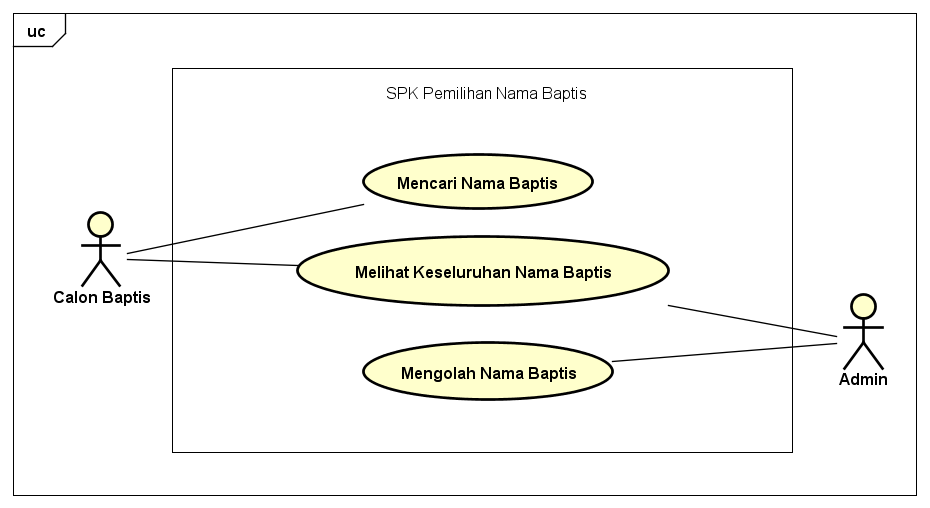
\includegraphics[scale=0.7]{usecase.PNG}
			\caption{\textit{Diagram \textit{Use Case} SPK Pemilihan Nama Baptis}}
		\label{fig:usecase}
	\end{figure}

	Berdasarkan hasil analisis  pada subbab analisis kuesioner, dibentuk 3 \textit{use case} dengan 2 aktor, antara lain:
	\begin{itemize}
			\item \textbf{\textit{User}}
				\begin{itemize}
					\item \textbf{Mencari Nama Baptis}

					Calon baptis dapat melihat dan atau memilih kategori apa saja yang dapat digunakan sebagai patokan untuk memilih nama baptis yang cocok, memasukkan \textit{input} seperti kata kunci, dan melihat hasil \textit{output} berupa nama baptis dan deskripsinya. Kategori yang dapat dijadikan patokan atau acuan adalah tanggal lahir calon baptis, tanggal pesta santo-santa, lambang santo-santa, arti nama dari santo-santa, tanggal pembaptisan, deskripsi dari santo-santa, dan profesi dari santo-santa.
					%\item \textbf{Memasukkan \textit{Input}}

					%Calon baptis dapat memasukkan \textit{Input} seperti kata kunci untuk mencari nama baptis yang mereka inginkan.
					%\item \textbf{Melihat Hasil \textit{Output}}

					%Calon baptis dapat melihat hasil \textit{Output} yang dijadikan sebagai alternatif pemilihan nama baptis. Terlebih dahulu calon baptis memasukkan kata kunci dan juga kategori yang diinginkan untuk dijadikan pedoman, agar alternatif dapat dihasilkan dan calon baptis tersebut dapat memilih nama baptis yang diinginkan.
					\item \textbf{Melihat Keseluruhan Nama Baptis}

					Calon baptis atau pengguna umum dapat melihat keseluruhan nama baptis beserta deskripsi di dalamnya.
				\end{itemize}
			\item \textbf{Admin}
				\begin{itemize}
				\item \textbf{Melihat Keseluruhan Nama Baptis}

					Admin dapat melihat keseluruhan nama baptis beserta deskripsi di dalamnya.
					
					\item \textbf{Mengolah Nama Baptis}

					Admin dapat melakukan \textit{update} atau memperbaharui nama baptis, menambahkan nama baptis, dan menghapus nama baptis. Admin dapat memperbaharui nama baptis, serta informasi atau deskripsi yang ada di dalamnya, seperti arti, lambang, profesi dari santo-santa tersebut dan lain sebagainya. Selain dapat memperbaharui, admin juga dapat menambahkan dan menghapus nama baptis serta informasi yang ada di dalamnya.
					%\item \textbf{Menambahkan Nama Baptis}

					%Admin dapat menambahkan nama baptis, dan juga deskripsi atau informasi di dalamnya.
					%\item \textbf{Menghapus Nama Baptis}

					%Admin dapat menghapus nama baptis yang sekiranya tidak terlalu lengkap informasinya.
				\end{itemize}
	\end{itemize}
	
\textbf{Skenario \textit{Use Case}}
\label{sec:skenariousecase}
\begin{enumerate}
\item \textit{User}


                       \begin{enumerate}
                        \item Mencari Nama Baptis
                                \begin{itemize}
                                        \item Nama: Mencari Nama Baptis
                                        \item Aktor: Calon Baptis
                                        \item Deskripsi: Memilih kategori, memasukkan \textit{input}, dan dapat melihat hasil \textit{output} yang sesuai dengan yang dinginkan oleh calon baptis.
                                        \item Kondisi awal: Calon baptis telah membuka web pemilihan nama baptis dan telah memilih kategori, serta memasukkan \textit{input} berupa kata kunci. %msh bingung
                                        \item Kondisi akhir: Web akan menampilkan nama baptis yang dapat dipilih oleh calon baptis.%msh bingung
                                        \item Skenario utama:														
				
				\begin{center}
  \begin{tabular}{ | c | p{6cm} |p{6cm} |}
    \hline
    No  & Aksi & Reaksi Sistem\\ \hline 
		1 & Calon baptis memilih kategori yang telah disediakan, 
		seperti tanggal lahir, profesi, arti dan lain sebagainya. %beserta
		%kata kunci agar memudahkan calon baptis memilih alternatif yang telah di keluarkan. 
		&  Sistem mendapatkan data dari calon baptis berupa kategori yang dipilih.\\ \hline 
		2 & Calon baptis memasukkan \textit{input} berupa kata kunci. & Sistem mendapatkan data dari calon baptis berupa kata kunci dan menampilkan hasil pencarian berdasarkan kata kunci.
		\\ \hline
		
		3 & Calon baptis melihat dan memilih hasil \textit{output} berupa alternatif nama baptis. & Tidak ada reaksi sistem.\\ \hline
		
    \end{tabular}
\end{center} 

                                \end{itemize}
                        %\item Memasukkan \textit{Input}

%			\begin{itemize}
 %                                       \item Nama: Memasukkan \textit{input}
  %                                      \item Aktor: Calon Baptis
   %                                     \item Deskripsi: Memasukkan input berupa kata kunci atau kata yang akan dicari sebagai acuan atau pedoman calon baptis.
    %                                    \item Kondisi awal: calon baptis telah memilih kategori %msh bingung
     %                                   \item Kondisi akhir: web akan menampilkan halaman alternatif nama baptis (\textit{output}) %msh bingung
      %                                  \item Skenario utama:														
				
				%\begin{center}
			  %\begin{tabular}{ | c | p{5cm} |p{5cm} |}
			  %  \hline
			  %  No  & Aksi & Reaksi Sistem\\ \hline 
				%1 & Calon baptis memasukkan kata kunci atau kata yang ingin dicari. % agar memudahkan calon baptis memilih alternatif yang telah di keluarkan. 
				%&  Sistem mendapatkan data dari calon baptis berupa kata kunci atau kata yang dicari, kemudian menampilkan halaman alternatif nama baptis.\\ \hline 
			   % \end{tabular}
		%	\end{center} 

     %                   \item Eksepsi: Calon baptis ingin memilih nama baptis yang cocok %msh bingung
%                                \end{itemize}

 %                       \item Melihat Hasil \textit{Output}

  %                      \begin{itemize}
   %                                     \item Nama: Melihat hasil \textit{output}
    %                                    \item Aktor: Calon Baptis
     %                                   \item Deskripsi: Melihat hasil \textit{output} yang sesuai dengan yang diinginkan calon baptis, setelah calon baptis memilih kategori dan memasukkan kata kunci.
      %                                  \item Kondisi awal: calon baptis telah memilih kategori dan kata kunci atau kata yang dicari  %msh bingung
       %                                 \item Kondisi akhir: calon baptis dapat memilih nama baptis berdasarkan alternatif yang telah keluar sebagai hasil (\textit{output}) %msh bingung
        %                                \item Skenario utama:														
				
				%\begin{center}
			  %\begin{tabular}{ | c | p{5cm} |p{5cm} |}
			   % \hline
			    %No  & Aksi & Reaksi Sistem\\ \hline 
				%1 & Calon baptis melihat dan memilih hasil \textit{output} berupa alternatif nama baptis.% agar memudahkan calon baptis memilih alternatif yang telah di keluarkan. 
				%&  Sistem menyusun dan mengurutkan data alternatif tersebut berdasarkan alternatif utama yang mana bobotnya lebih besar.\\ \hline 
			   % \end{tabular}
			%\end{center} 

       %                 \item Eksepsi: Calon baptis ingin memilih nama baptis yang cocok %msh bingung
        %                        \end{itemize}
                        \item Melihat Keseluruhan Nama Baptis

                         \begin{itemize}
                                        \item Nama: Melihat keseluruhan nama baptis
                                        \item Aktor: Calon Baptis atau pengguna umum
                                        \item Deskripsi: Melihat nama baptis dan informasinya
                                        \item Kondisi awal: calon baptis atau pengguna umum telah membuka web pemilihan nama baptis  %msh bingung
                                        \item Kondisi akhir: calon baptis atau pengguna umum dapat melihat nama baptis serta informasinya %msh bingung
                                        \item Skenario utama:														
				
				\begin{center}
			  \begin{tabular}{ | c | p{5cm} |p{5cm} |}
			    \hline
			    No  & Aksi & Reaksi Sistem\\ \hline 
				1 & Calon baptis atau pengguna umum memilih menu semua nama baptis.% agar memudahkan calon baptis memilih alternatif yang telah di keluarkan. 
				&  Sistem menampilkan seluruh nama baptis.\\ \hline 
			    \end{tabular}
			\end{center} 

                        
                                \end{itemize}
																\end{enumerate}
																\item Admin
																\begin{enumerate}
																\item Melihat Keseluruhan Nama Baptis
									
                         \begin{itemize}
                                        \item Nama: Melihat keseluruhan nama baptis
                                        \item Aktor: Admin
                                        \item Deskripsi: Melihat nama baptis dan informasinya
                                        \item Kondisi awal: Admin telah membuka web pemilihan nama baptis  %msh bingung
                                        \item Kondisi akhir: Admin dapat melihat nama baptis serta informasinya %msh bingung
                                        \item Skenario utama:														
				
				\begin{center}
			  \begin{tabular}{ | c | p{5cm} |p{5cm} |}
			    \hline
			    No  & Aksi & Reaksi Sistem\\ \hline 
				1 & Admin memilih menu semua nama baptis.% agar memudahkan calon baptis memilih alternatif yang telah di keluarkan. 
				&  Sistem menampilkan seluruh nama baptis.\\ \hline 
			    \end{tabular}
			\end{center}
																
																       \end{itemize}
																
                                \item Mengolah Nama Baptis
\begin{itemize}
\item Memperbaharui Nama Baptis
\begin{itemize}
                                        \item Nama: Memperbaharui Nama Baptis
                                        \item Aktor: Admin
                                        \item Deskripsi: Dapat memperbaharui data yang sudah ada sebelumnya, menambahkan data baru, dan menghapus data yang tidak terpakai.
                                        \item Kondisi awal: Data lama sudah terdapat pada sistem. %msh bingung
                                        \item Kondisi akhir: Data lama telah diperbaharui dengan data baru. %msh bingung
                                        \item Skenario utama:														
				
				\begin{center}
			  \begin{tabular}{ | c | p{5cm} |p{5cm} |}
			    \hline
			    No  & Aksi & Reaksi Sistem\\ \hline 
				1 & Admin mengubah nama baptis dan informasinya.% agar memudahkan calon baptis memilih alternatif yang telah di keluarkan. 
				&  Sistem akan mengubah nama baptis dan informasi lama menjadi sesuai dengan \textit{input} admin.\\ \hline 
			    \end{tabular}
			\end{center} 

                                \end{itemize}
		\item Menambahkan Nama Baptis

                                \begin{itemize}
                                        \item Nama: Menambahkan nama baptis
                                        \item Aktor: Admin
                                        \item Deskripsi: Dapat menambahkan data baru
                                        \item Kondisi awal: data belum ada pada sistem %msh bingung
                                        \item Kondisi akhir: data baru sudah ditambahkan dan akan ditampilkan%msh bingung
                                        \item Skenario utama:														
				
				\begin{center}
			  \begin{tabular}{ | c | p{5cm} |p{5cm} |}
			    \hline
			    No  & Aksi & Reaksi Sistem\\ \hline 
				1 & Admin menambahkan nama baptis beserta informasinya.% agar memudahkan calon baptis memilih alternatif yang telah di keluarkan. 
				&  Sistem akan menambahkan nama baptis beserta informasinya.\\ \hline 
			    \end{tabular}
			\end{center} 

                                \end{itemize}
																\item Menghapus Nama Baptis

                                \begin{itemize}
                                        \item Nama: Menghapus nama baptis
                                        \item Aktor: Admin
                                        \item Deskripsi: Dapat menghapus data yang terlihat tidak begitu lengkap atau tidak begitu terpakai.
                                        \item Kondisi awal: sebelumnya terdapat data pada sistem %msh bingung
                                        \item Kondisi akhir: data telah dihapus dan tidak akan muncul di tampilan%msh bingung
                                        \item Skenario utama:														
				
				\begin{center}
			  \begin{tabular}{ | c | p{5cm} |p{5cm} |}
			    \hline
			    No  & Aksi & Reaksi Sistem\\ \hline 
				1 & Admin menghapus nama baptis dan informasinya.% agar memudahkan calon baptis memilih alternatif yang telah di keluarkan. 
				&  Sistem akan menghapus nama baptis dan informasinya yang telah dipilih oleh admin.\\ \hline 
			    \end{tabular}
			\end{center} 

\end{itemize}

                                 
                                
                                
                                \end{itemize}
                \end{enumerate}

\end{enumerate}
\item Membuat desain web SPK Pemilihan nama baptis Katolik.\\
		{\bf status :} Ada sejak rencana kerja skripsi.\\
		{\bf hasil :}
		
\textbf{Tampilan \textit{Home}}
		
		Pada tampilan \textit{home} (Gambar \ref{fig:home}: Tampilan \textit{Home}), terdapat deskripsi mengenai pembaptisan secara umum dan singkat. Selain deskripsi, terdapat gambar berupa macam-macam pembaptisan. Gambar tersebut menggunakan slider, agar \textit{user} dapat mengerti gambaran mengenai proses pembaptisan. Selain deskripsi dan gambar, pada tampilan \textit{home} juga terdapat beberapa pilihan, seperti \textit{home}, \textit{about}, nama baptis, dan \textit{contact}. Nama baptis tersebut mempunyai tampilan semua nama baptis dan tampilan kategori pemilihan nama baptis.
		
\begin{figure}[htbp]
		\centering
			\includegraphics[scale=0.34]{1.PNG}
			\caption{Tampilan \textit{Home}}
		\label{fig:home}
	\end{figure}

\textbf{Tampilan \textit{About}}
		
		Pada tampilan \textit{about} (Gambar \ref{fig:about}: Tampilan \textit{About}), terdapat deskripsi mengenai pembaptisa secara mendetail.
		
\begin{figure}[htbp]
		\centering
			\includegraphics[scale=0.34]{2.PNG}
			\caption{Tampilan \textit{About}}
		\label{fig:about}
	\end{figure}
	
	
	\textbf{Tampilan Semua Nama Baptis}
		
		Pada tampilan semua nama baptis (Gambar \ref{fig:semuanama}: Tampilan Semua Nama Baptis), terdapat berbagai macam nama baptis, gambar dari santo-santa, dan deskripsinya. Pada tampilan ini, semua orang termasuk orang awam dapat melihat berbagai macam nama baptis, beserta deskripsinya.
		
\begin{figure}[htbp]
		\centering
			\includegraphics[scale=0.34]{3.PNG}
			\caption{Tampilan Semua Nama Baptis}
		\label{fig:semuanama}
	\end{figure}
	
\textbf{Tampilan Kategori Pemilihan Nama Baptis}
		
		Pada tampilan kategori pemilihan nama baptis (Gambar \ref{fig:pemilihan}: Tampilan Kategori Pemilihan Nama Baptis), terdapat berbagai macam pilihan kategori untuk memilih nama baptis yang tepat untuk seorang calon baptis yang ingin dibaptis. Kategori tersebut terdiri dari:
		
		\begin{itemize}
			\item Arti Nama Santo-Santa
			\item Deskripsi (Cerita Kehidupan) Santo-Santa
			\item Tanggal Lahir Calon Baptis
			\item Tanggal Pembaptisan Calon Baptis
			\item Profesi Santo-Santa
			\item Lambang Santo-Santa
			\item Tanggal Pesta Santo-Santa (tanggal peringatan)
		\end{itemize}
		
		Selain kategori tersebut, terdapat juga sebuah \textit{button} yang berguna untuk mencari nama baptis, berdasarkan kategori yang telah dicari oleh calon baptis (\textit{user}). Setelah \textit{user} menekan \textit{button} cari, maka akan keluar sebuah \textit{output}, yang mendekati atau sama dengan yang diinginkan oleh \textit{user}.
\begin{figure}[htbp]
		\centering
			\includegraphics[scale=0.34]{4.PNG}
			\caption{Tampilan Kategori Pemilihan Nama Baptis}
		\label{fig:pemilihan}
	\end{figure}

\item Menulis dokumen skripsi.\\
		{\bf status :} Ada sejak rencana kerja skripsi.\\
		{\bf hasil :} Sebagian dokumen skripsi dari Bab 2, dan Bab 3 sudah dikerjakan. Hasil pengerjaan dokumen skripsi Bab 2 dapat dilihat pada perkembangan pengerjaan skripsi nomor 5-9, 11, sedangkan hasil pengerjaan dokumen skripsi Bab 3 dapat dilihat pada nomor 1-4, 10, 12-14.

\bibliographystyle{ieeetr}
\bibliography{pustaka}


\textbf{Lampiran}

\textbf{Formulir Pertanyaan Kuesioner}

\begin{figure}[htbp]
		\centering
			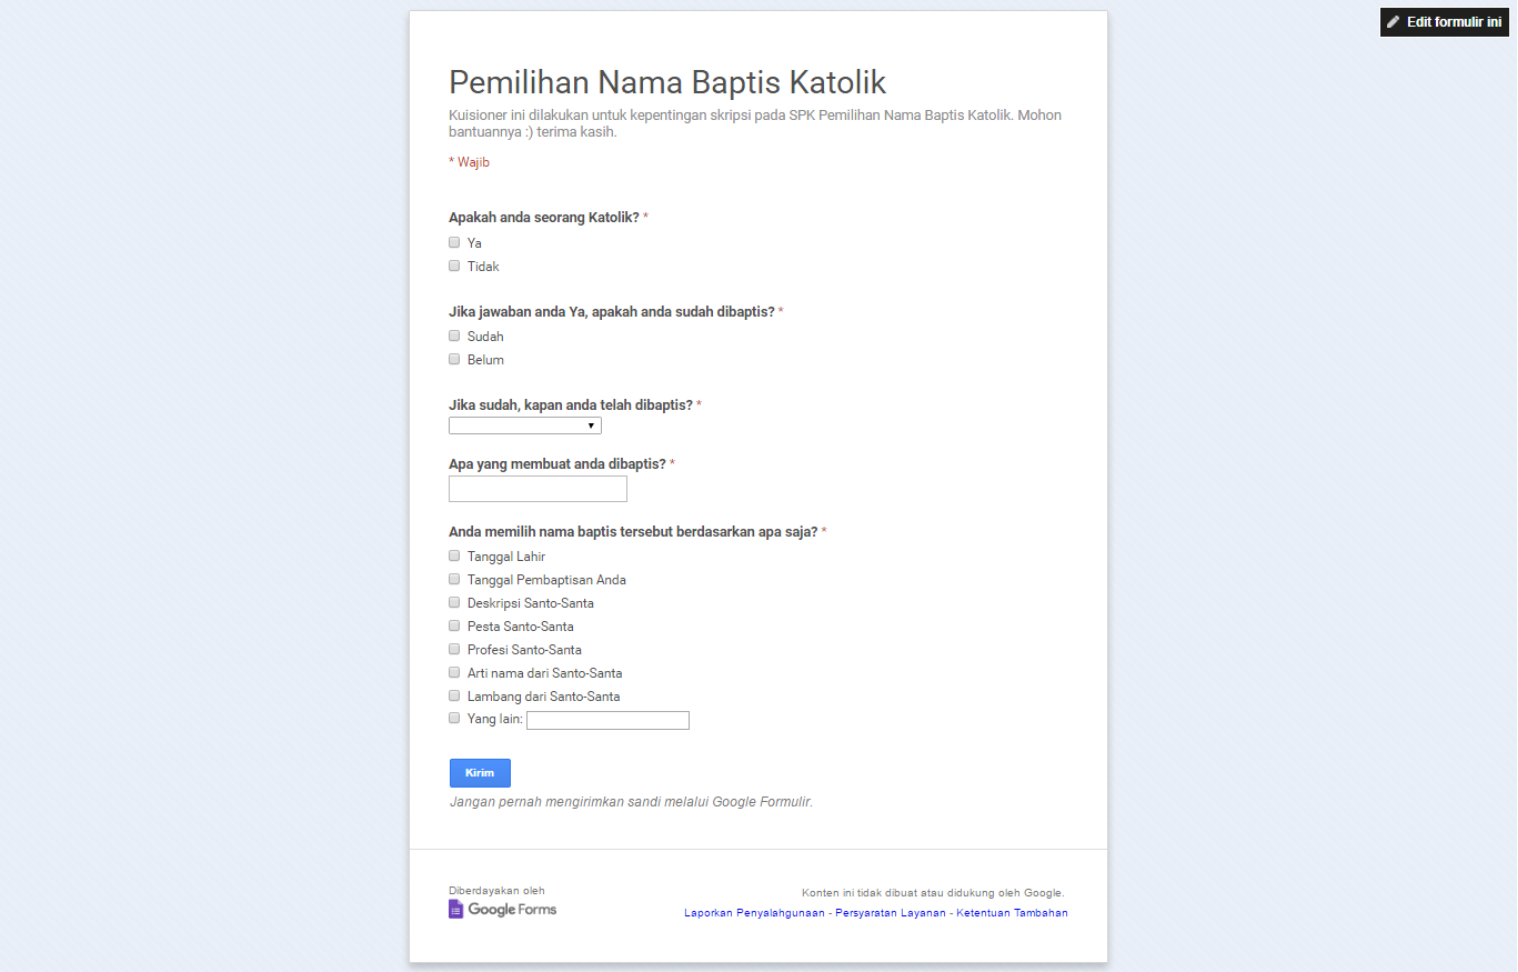
\includegraphics[scale=0.34]{formkuesioner.PNG}
			\caption{Formulir Pertanyaan Kuesioner}
		\label{fig:formkuesioner}
	\end{figure}


\textbf{Hasil Kuesioner}

\begin{figure}[htbp]
		\centering
			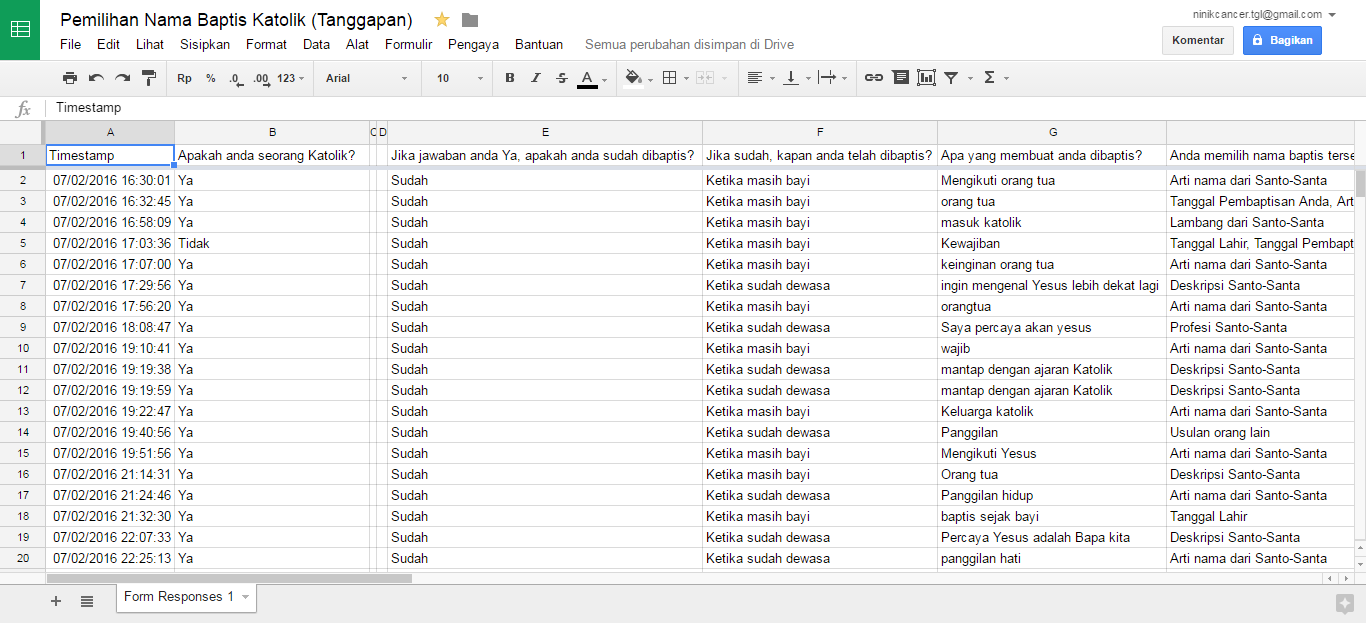
\includegraphics[scale=0.38]{kuesioner1.PNG}
			\caption{Hasil Kuesioner}
		\label{fig:kues1}
	\end{figure}
	
	\begin{figure}[htbp]
		\centering
			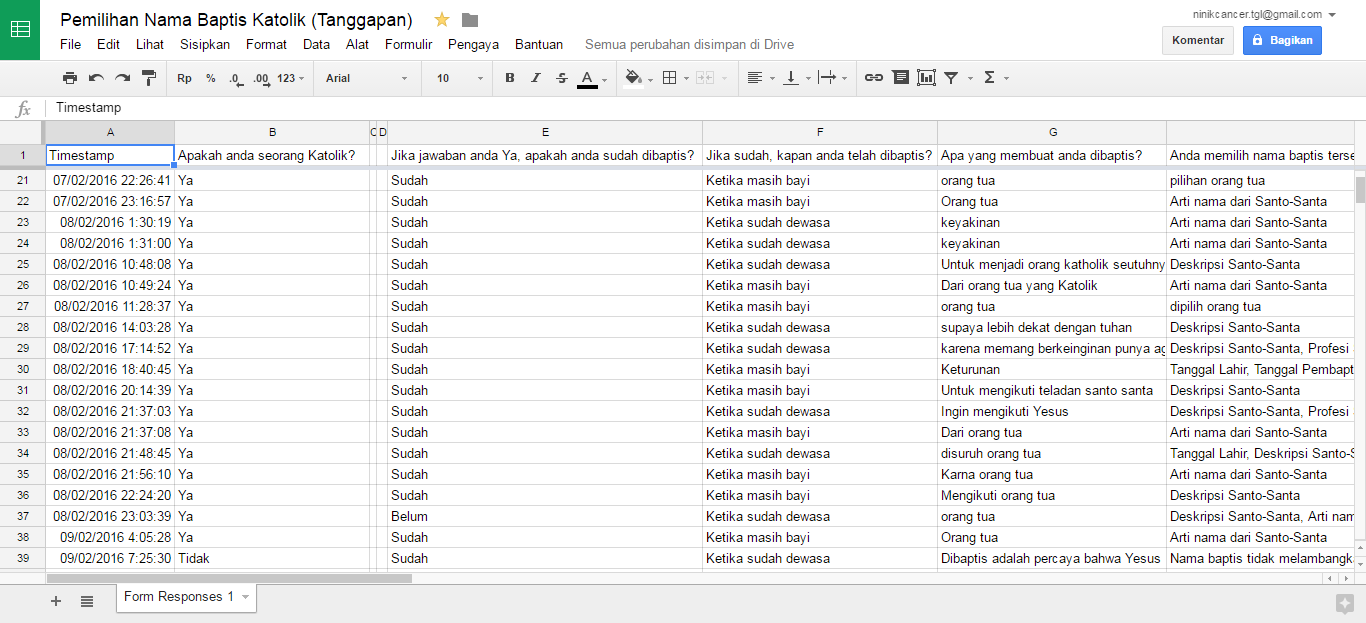
\includegraphics[scale=0.38]{kuesioner2.PNG}
			\caption{Hasil Kuesioner}
		\label{fig:kues2}
	\end{figure}
	
	\begin{figure}[htbp]
		\centering
			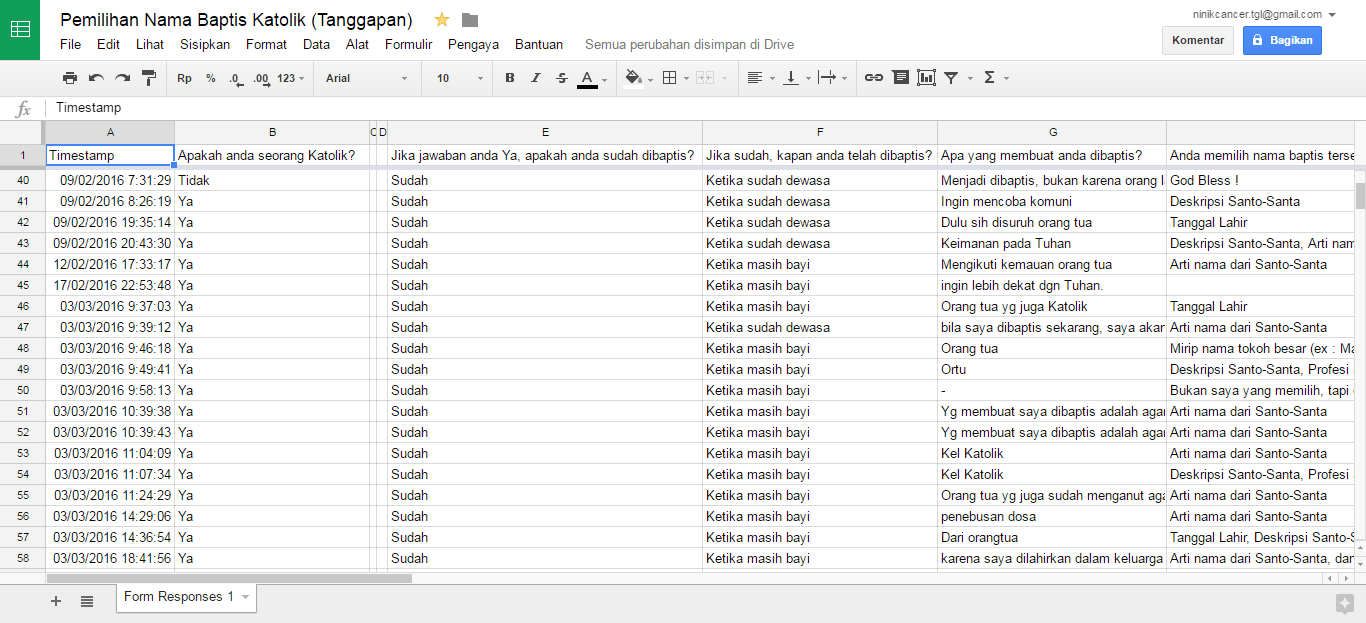
\includegraphics[scale=0.38]{kuesioner3.PNG}
			\caption{Hasil Kuesioner}
		\label{fig:kues3}
	\end{figure}
	
	\begin{figure}[htbp]
		\centering
			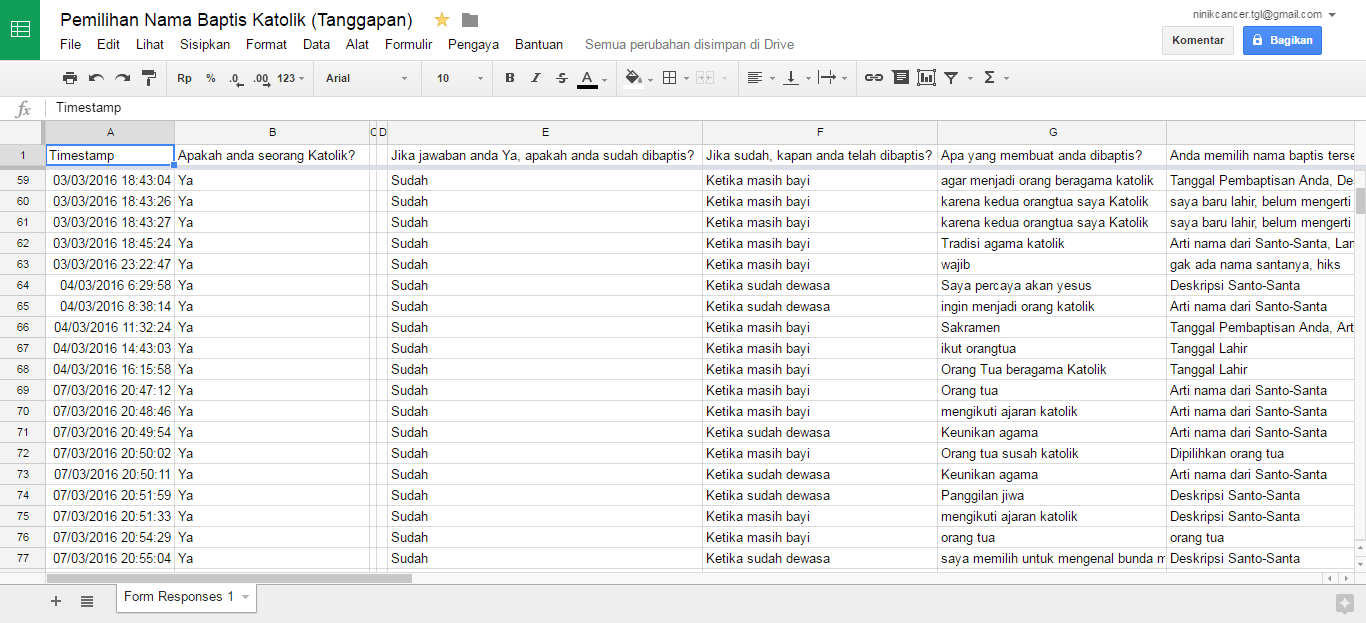
\includegraphics[scale=0.38]{kuesioner4.PNG}
			\caption{Hasil Kuesioner}
		\label{fig:kues4}
	\end{figure}
	
	\begin{figure}[htbp]
		\centering
			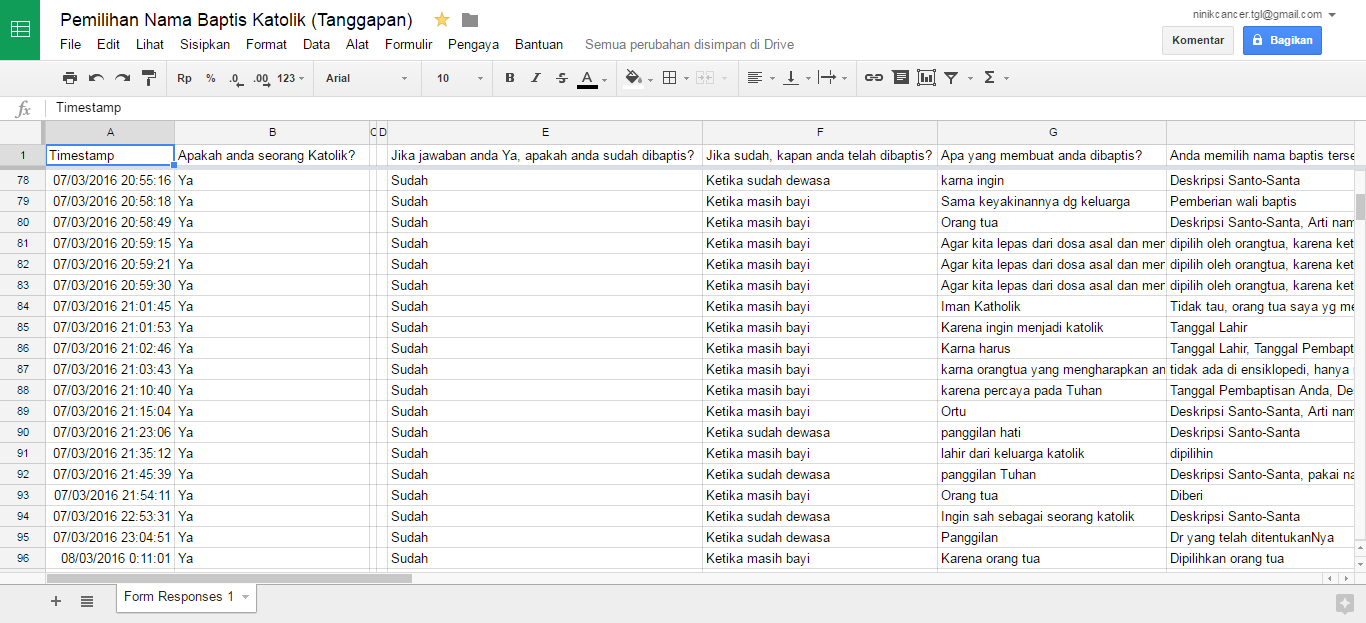
\includegraphics[scale=0.38]{kuesioner5.PNG}
			\caption{Hasil Kuesioner}
		\label{fig:kues5}
	\end{figure}
	
	\begin{figure}[htbp]
		\centering
			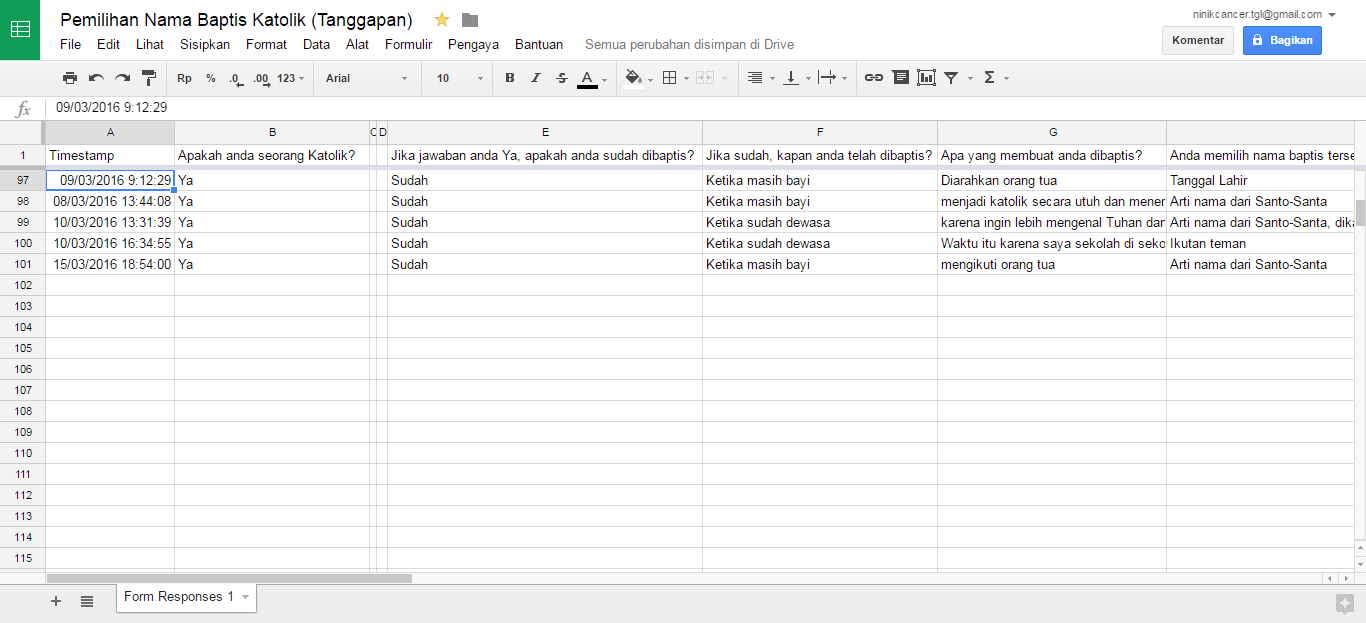
\includegraphics[scale=0.38]{kuesioner6.PNG}
			\caption{Hasil Kuesioner}
		\label{fig:kues6}
	\end{figure}

\textbf{Bukti Wawancara
}
	\begin{figure}[htbp]
		\centering
			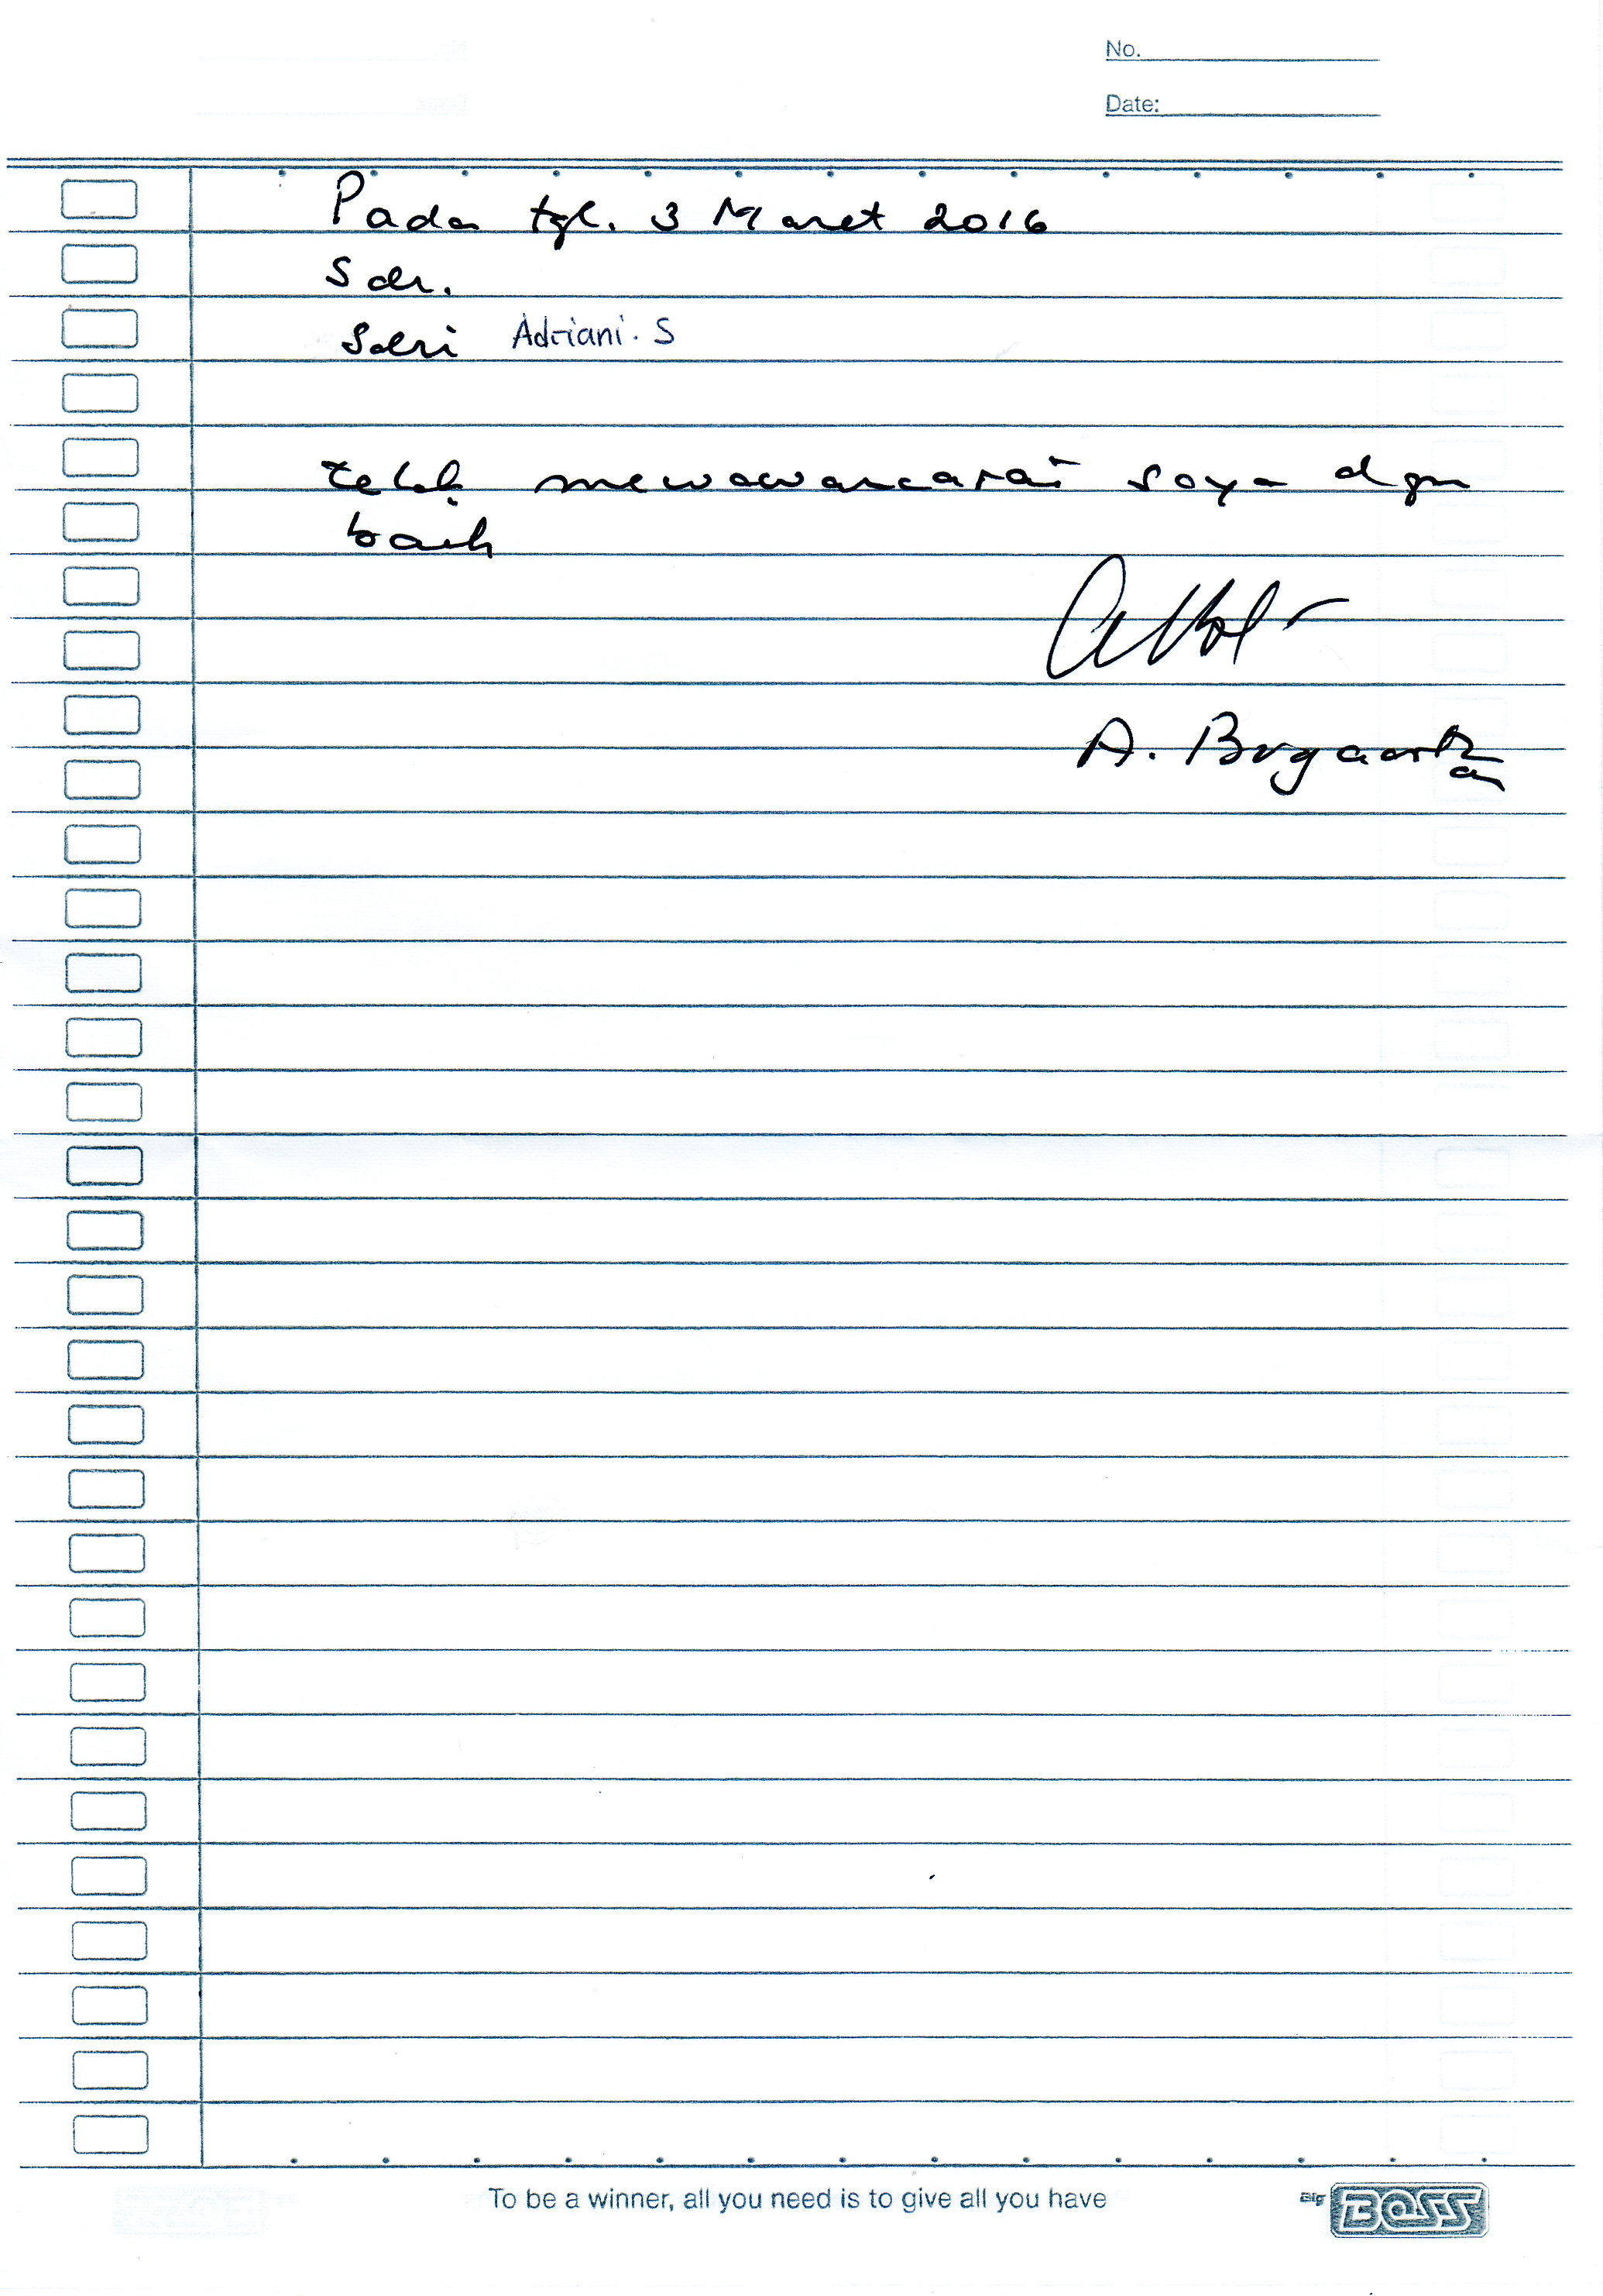
\includegraphics[scale=0.6]{sc0006.JPG}
			\caption{Bukti Wawancara}
		\label{fig:bukti}
	\end{figure}

	
\textbf{Nama Baptis}

\begin{figure}[htbp]
		\centering
			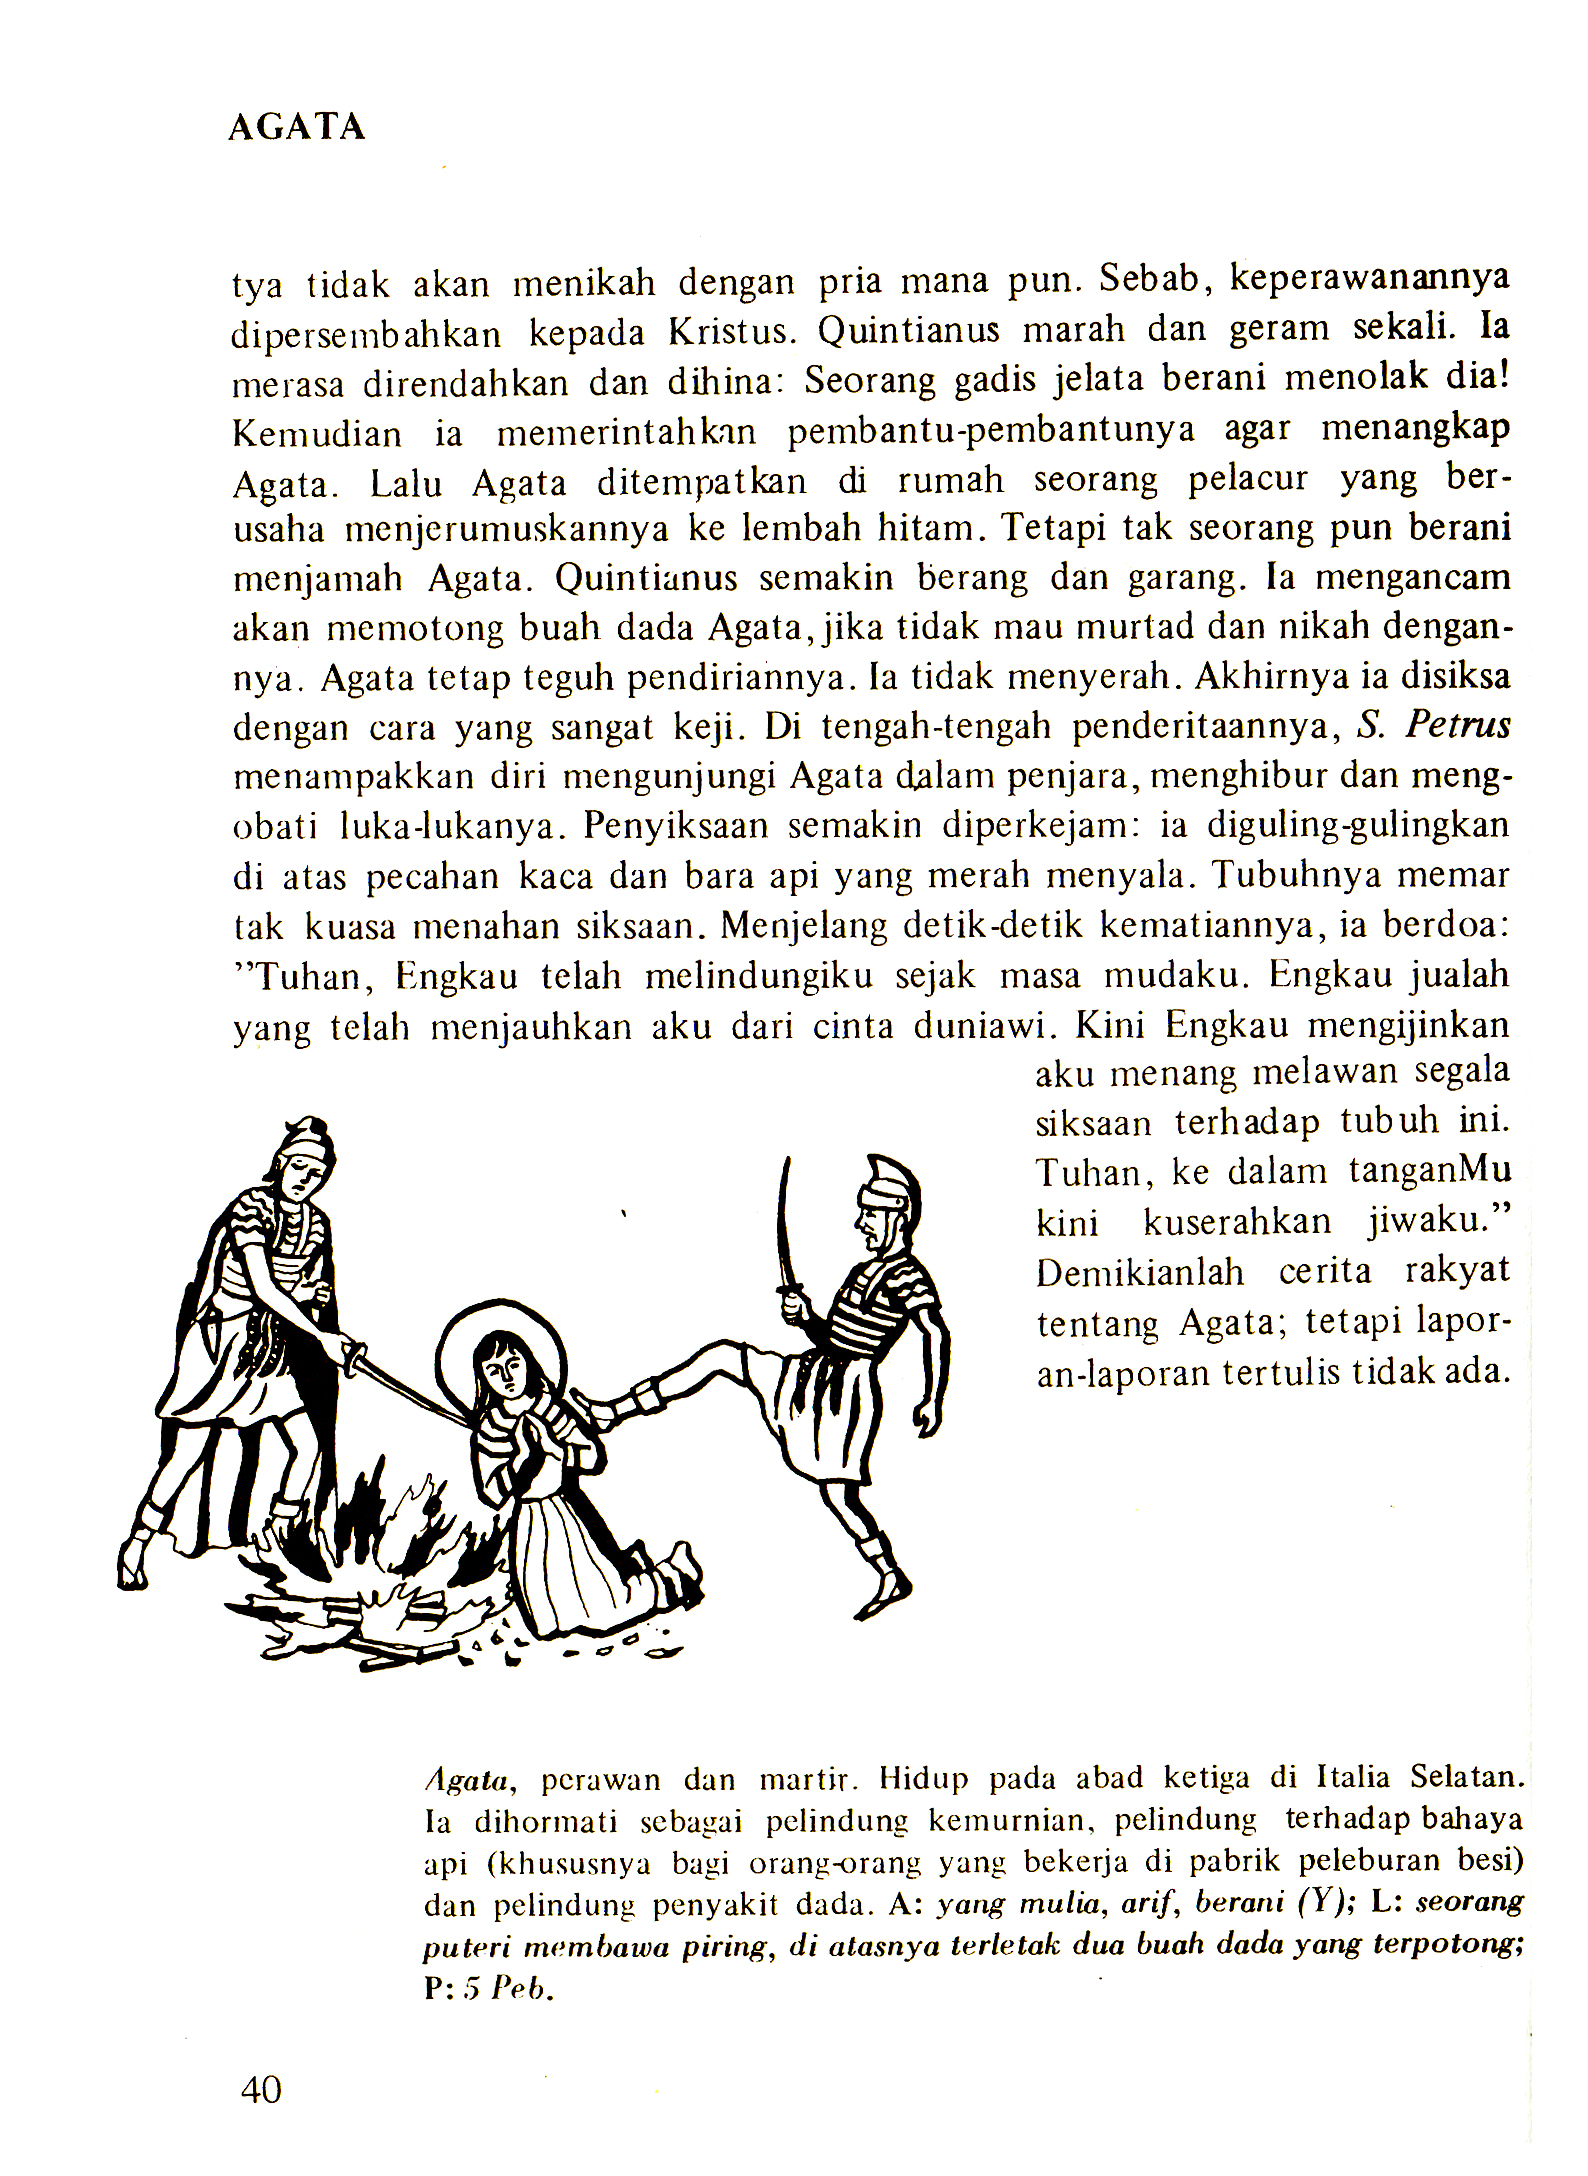
\includegraphics[scale=0.9]{sc0004.JPG}
			\caption{Nama Baptis}
		\label{fig:namabaptis1}
	\end{figure}
	
\begin{figure}[htbp]
		\centering
			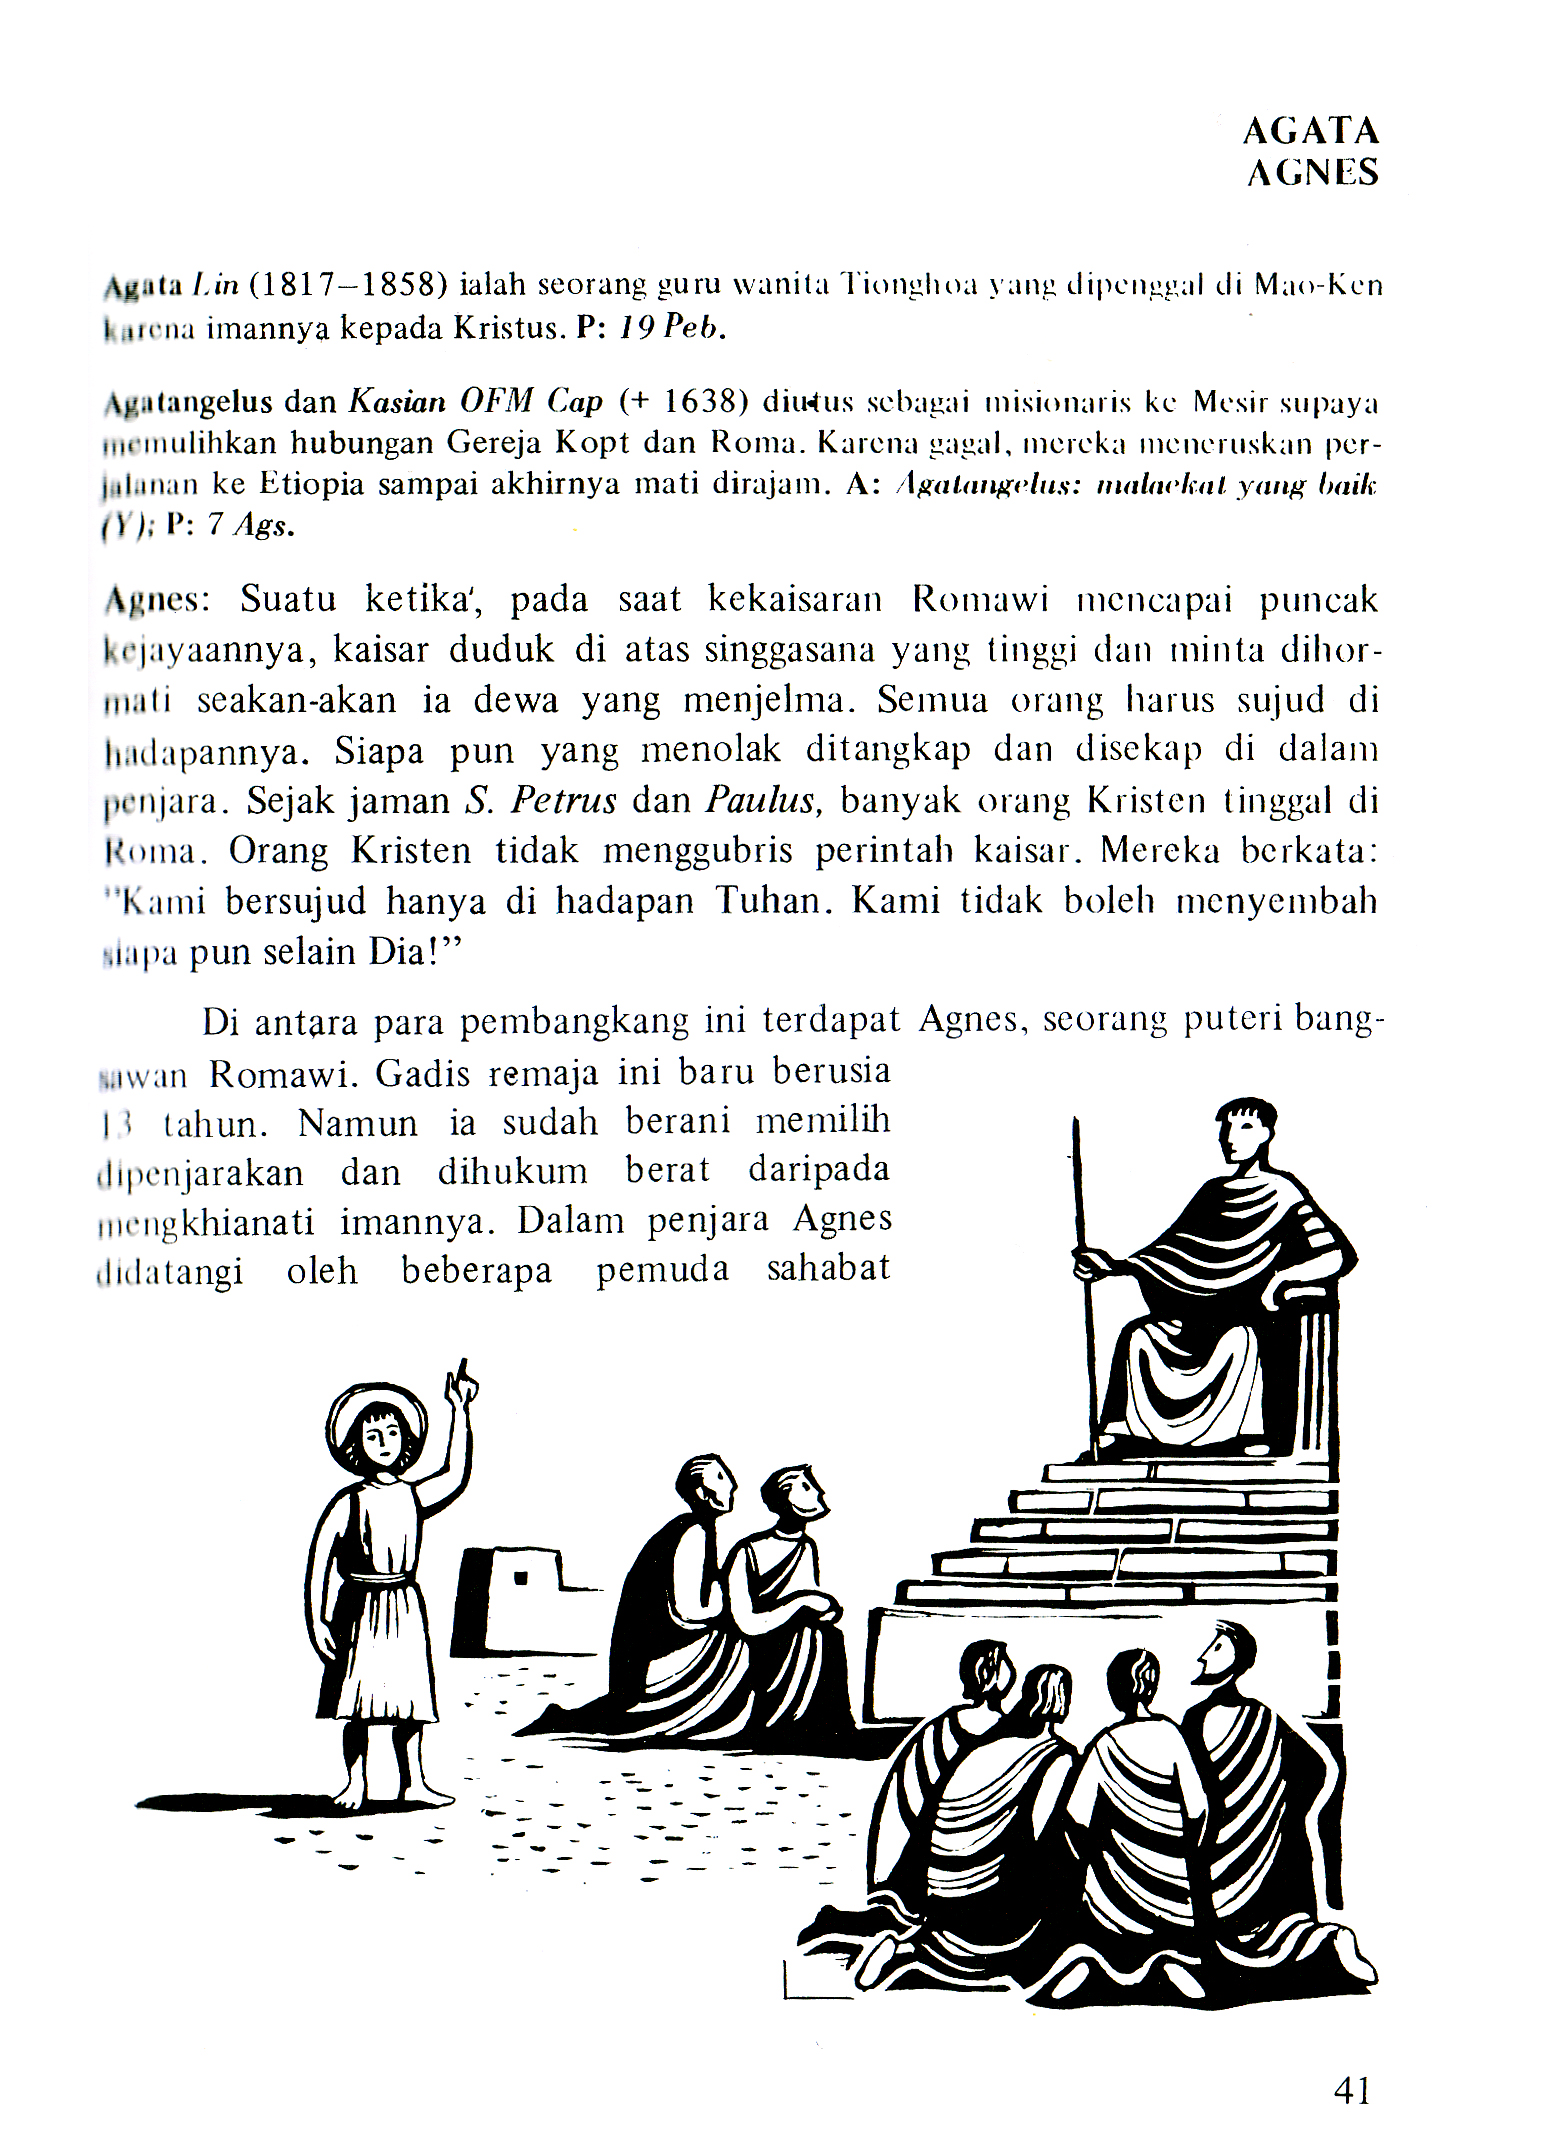
\includegraphics[scale=0.9]{sc0005.JPG}
			\caption{Nama Baptis}
		\label{fig:namabaptis2}
	\end{figure}

%\end{lstlisting}
	
	
	%	\item Melakukan studi literatur mengenai metode SPK lainnya, seperti AHP, MAGIQ, WP, ELECTRE, TOPSIS.\\
	%	{\bf status :} Baru ditambahkan semester ini.\\
	%	{\bf hasil :} 

	%	\item Mempelajari bahasa pemrograman C++ dan cara menggunakan framework OpenSteer\\
	%	{\bf status :} Ada sejak rencana kerja skripsi.\\
		%{\bf hasil :}
%		\item Merancang pergerakan kerumunan di dalam museum menggunakan teknik {\it social force model} dan {\it flow tiles} serta menggunakan teknik lainnya seperti konsep pathway dan waypoints. Selain itu, dirancang pula adanya waktu tunggu (pada saat pengunjung melihat objek di museum) dan cara pembuatan jalur bagi setiap individu pengunjung\\
		%{\bf status :} Ada sejak rencana kerja skripsi.\\
		%{\bf hasil :}

		%\item Melakukan analisa dan merancang struktur data yang cocok untuk menyimpan penghalang (obstacle)\\
		%{\bf status :} dihapuskan/tidak dikerjakan \\
	%	{\bf hasil :} berdasarkan analisis singkat, tidak dilakukan analisis lebih jauh karena tidak diperlukan struktur data baru, karena sudah disediakan oleh OpenSteer versi terbaru

		%\item Mengimplementasikan keseluruhan algoritma dan struktur data yang dirancang, dengan menggunakan framework OpenSteer \\
		%{\bf status :} Ada sejak rencana kerja skripsi.\\
		%{\bf hasil :}
%		\item Melakukan pengujian (dan eksperimen) yang melibatkan responde untuk menilai hasil simulasi secara kualitatif\\
	%	{\bf status :} Ada sejak rencana kerja skripsi.\\
	%	{\bf hasil :}

	%	\item Menulis dokumen skripsi\\
	%	{\bf status :} Ada sejak rencana kerja skripsi.\\
		%{\bf hasil :} \lipsum[1]
	%		\item Mempelajari cara menggunakan fitur manipulasi obstacle yang disediakan oleh framework Opensteer versi terbaru\\
		%{\bf status :} baru ditambahkan pada semester ini\\
	%	{\bf hasil :} baru direncanakan karena framework Opensteer versi paling akhir baru selesai diinstall dan dilihat-lihat bagian contoh-contoh simulasinya
		

	\end{enumerate}

\section{Pencapaian Rencana Kerja}
Persentase penyelesaian skripsi sampai dengan dokumen ini dibuat dapat dilihat pada tabel berikut :

\begin{center}
  \begin{tabular}{ | c | c | c | c | l | c |}
    \hline
    1*  & 2*(\%) & 3*(\%) & 4*(\%) &5* &6*(\%)\\ \hline \hline
    1   & 5  & 5  &  &  & 5 \\ \hline
    2   & 5 & 5  &   & & 5\\ \hline
    3   & 20  & 15  &5  &  {\footnotesize studi literatur mengenai metode SAW dan bootstrap pada skripsi 1}&15 \\ \hline
    4   & 10  & 10  &   & &10 \\ \hline
    5   & 15  &   & 15 &  &15\\ \hline
		6		& 30  &   & 30 &  &\\ \hline
    7   & 5 &  & 5  & &\\ \hline
    8   & 15  & 5  & 10 & {\footnotesize mengerjakan bab 1 dan bab 2 pada skripsi 1} & \\ \hline
    Total  & 100  & 40  & 60 & &  \\ \hline
                          \end{tabular}
\end{center}

Keterangan (*)\\
1 : Bagian pengerjaan Skripsi (nomor disesuaikan dengan detail pengerjaan di bagian 5)\\
2 : Persentase total \\
3 : Persentase yang akan diselesaikan di Skripsi 1 \\
4 : Persentase yang akan diselesaikan di Skripsi 2 \\
5 : Penjelasan singkat apa yang dilakukan di S1 (Skripsi 1) atau S2 (skripsi 2)\\
6 : Persentase yang sidah diselesaikan sampai saat ini 

%\section{Kendala yang dihadapi}
%TULISKAN BAGIAN INI JIKA DOKUMEN ANDA TIPE A ATAU C
%Kendala - kendala yang dihadapi selama mengerjakan skripsi :
%\begin{itemize}
	%\item Terlalu banyak melakukan prokratinasi
	%\item Terlalu banyak godaan berupa hiburan (game, film, dll)
	%\item Skripsi diambil bersamaan dengan kuliah ASD karena selama 5 semester pertama kuliah tersebut sangat dihindari dan tidak diambil, dan selama 4 semester terakhir kuliah tersebut selalu mendapat nilai E
	%\item Mengalami kesulitan pada saat sudah mulai membuat program komputer karena selama ini selalu dibantu teman
%\end{itemize}

\vspace{1cm}
\centering Bandung, \tanggal\\
\vspace{2cm} \nama \\ 
\vspace{1cm}

Menyetujui, \\
\ifdefstring{\jumpemb}{2}{
\vspace{1.5cm}
\begin{centering} Menyetujui,\\ \end{centering} \vspace{0.75cm}
\begin{minipage}[b]{0.45\linewidth}
% \centering Bandung, \makebox[0.5cm]{\hrulefill}/\makebox[0.5cm]{\hrulefill}/2013 \\
\vspace{2cm} Nama: \pembA \\ Pembimbing Utama
\end{minipage} \hspace{0.5cm}
\begin{minipage}[b]{0.45\linewidth}
% \centering Bandung, \makebox[0.5cm]{\hrulefill}/\makebox[0.5cm]{\hrulefill}/2013\\
\vspace{2cm} Nama: \pemB \\ Pembimbing Pendamping
\end{minipage}
\vspace{0.5cm}
}{
% \centering Bandung, \makebox[0.5cm]{\hrulefill}/\makebox[0.5cm]{\hrulefill}/2013\\
\vspace{2cm} Nama: \pembA \\ Pembimbing Tunggal
}

\end{document}

